% This document does not intend to be an everything-in-one document for
% creating the diploma paper. However it does the most meaningful work
% for you.
%
% You can get the full document list on your cathedra or use the following 
% (order preserved)
%
% 1.  Title page
% 2.  General task.
% 3.  Plan.
% 4.  Separate sections consults (for ex.: ecology and labour protection).
% 5.  Technical task.
% 6.  Annotation.
% 7.  Nomenclature list.
% 8.  Table of Contents.
% 9.  Diploma paper itself.
% 10. Conclusions.
% 11. Reference list.
% 12. Appendixes.
% Andriy Senkovych
%
% Many thanks to my friend Andriy, for this template, original comments saved
% 

\documentclass[ukrainian,utf8,simple,floatsubsection, hpadding=5mm,equationsubsection,]{eskdtext}
% hpadding=5mm  intend between frame and text, by default 3mm
% hpadding=5mm  відступ між початком і кінцем стрічки тексту та рамкою, по замовчанню 3 мм
% equationsubsection enumerate formula based on subsection



\usepackage[warn]{mathtext}
\usepackage[unicode]{hyperref} % enable hyperlinks (активувати посилання)

% Formulae + cyrillic = wtf???
% You should use \text{} in formulae to write cyrillic characters. 
% Unfortunately mathtext package is not supported :(
% Example: $ \text{а} + \text{б} = \text{в} $

% explanation for formulas should be in next form:
% \begin{ESKDexplanation}
%     \item  [something]
%     \item  [something else]
% \end{ESKDexplanation}


\usepackage{amssymb} % special math characters
\usepackage{amsmath} % using cyrillic in formulae
\usepackage{amsfonts} % special math fonts

\usepackage{eskdtotal} % calculate total number of pages, figures, tables and etc.
% You should use \ESKDtotal{page} to count number of pages in Diploma
% \ESKDtotal{figure} to count number of figures
% \ESKDtotal{bibitem} - count number of references

\usepackage{graphicx,epstopdf} % epstopdf-convert eps files to pdf
\graphicspath{{algorithms/}{schemes/}{software/}{fig/}} % look up folders for figures




\usepackage{listings} % to add source codes

\usepackage{longtable} % multipage tables
\usepackage{multirow} % using rowspan in tables

\usepackage{nomencl} % support for abbreviations
\makenomenclature % generate abbrevs index file

% variables.tex
% This file contains information about author and other specific
% people for use in eskdx collection.

\title{\fontsize{12}{12} \selectfont Інтегрована інерціально-супутникова система навігації, що базується на принципах комплексної обробки інформації
з використанням калманівської фільтрації}
% smaller size of font set for the title in frame
\author{НовікМ.В.}

\ESKDchecker{ФіляшкінМ.К.}
\ESKDnormContr{КозловА.П.}
\ESKDapprovedBy{СинєглазовВ.М.}

\ESKDdepartment{Міністерство освіти і науки України}
\ESKDcompany{Національний авіаційний університет}

\ESKDsignature{НАУ 11 09 02 000 ПЗ}
\ESKDgroup{ІАСУ 608}

\ESKDsectAlign{section}{Center}
\ESKDsectAlign{subsection}{Center}
\ESKDsectAlign{subsubsection}{Center}

 % class parameters tuning

\begin{document}

% Uncoment this to include task to the paper
%\ESKDthisStyle{formIIab}
%% \documentclass[ukrainian,utf8,simple,floatsingle,hpadding=5mm]{eskdtext}
% \usepackage[numberright]{eskdplain}
% % variables.tex
% This file contains information about author and other specific
% people for use in eskdx collection.

\title{\fontsize{12}{12} \selectfont Інтегрована інерціально-супутникова система навігації, що базується на принципах комплексної обробки інформації
з використанням калманівської фільтрації}
% smaller size of font set for the title in frame
\author{НовікМ.В.}

\ESKDchecker{ФіляшкінМ.К.}
\ESKDnormContr{КозловА.П.}
\ESKDapprovedBy{СинєглазовВ.М.}

\ESKDdepartment{Міністерство освіти і науки України}
\ESKDcompany{Національний авіаційний університет}

\ESKDsignature{НАУ 11 09 02 000 ПЗ}
\ESKDgroup{ІАСУ 608}

\ESKDsectAlign{section}{Center}
\ESKDsectAlign{subsection}{Center}
\ESKDsectAlign{subsubsection}{Center}


% \include{textcomp}
% \usepackage{longtable} % multipage tables
% \usepackage{multirow} % using rowspan in tables
% % Enumerations in listings use arabic numbers insted of letters
% \renewcommand\labelenumi{\arabic{enumi}.} 
% \renewcommand\labelenumii{\theenumi.\arabic{enumii}.}
% \renewcommand\labelenumiii{\arabic{enumi}.\arabic{enumii}.\arabic{enumiii}.}
% \ESKDstyle{formIIab}
% \begin{document}
% 
% \ESKDthisStyle{formII}


\subsection*{Технічне завдання}

\subsubsection*{1. Найменування та галузь застосування}

% В теперішній час визнано, що одним з основних шляхів вдосконалення навігаційного обладнання 
% є створення комплексних навігаційних систем, що інтегрують  командні прибори в єдиний блок, 
% здатний автоматично вирішувати задачу навігації ЛА. Сутність комплексування полягає у 
% використанні інформаційної та структурної надмірності для підвищення точності, надійності 
% та завадостійкості інформації при вимірюванні одних і тих же або функціонально зв’язаних 
% навігаційних параметрів. Інформаційна надмірність полягає в тому, що забезпечується отримання 
% однорідної інформації від декількох навігаційних датчиків різної фізичної природи з наступною 
% сумісною обробкою цієї інформації в спеціалізованому обчислювачі. Надмірність структури 
% комплексу забезпечує його працездатність при відмові, особливо короткотривалій, одного із датчиків. 
% 


Досить актуальною на даний час є задача створення комплексної навігаційної системи на базі супутникової та інерціальної систем навігації для визначення координат місця розташування рухливого об’єкта, у тому числі ЛА. Однією з центральних ідей розвитку навігаційного обладнання літальних апаратів  є функціональне, інформаційне й апаратурне об'єднання навігаційних вимірників в інтегрований навігаційний комплекс. Використання інтегрованих інерціально-супутникових систем компенсує недоліки окремих систем, і забезпечує високу точність і надійність виміру параметрів польоту.

Задача створення комплексної навігаційної системи на базі супутникової та інерціальної систем навігації длявизначення координат місце-положення рухомого об'єкта, передбачає попередній аналіз існуючих варіантів компонентів комплексної навігаційної системи, тобто варіантів побудови супутникової й  інерціальної систем навігації та вибір за певними критеріями найбільш оптимальних. Природно, що за головний критерій повинно бути обрано вартість системи та задана точність визначення координат рухомого об’єкта.

Найбільш привабливим для розв’язання цієї задачі є залучення калманівської фільтрації. 
Фільтр Калмана призначений для ідентифікації (оцінювання) змінних стану системи за даними 
вимірювання вихідних сигналів цієї системи, які містять похибки вимірювання (вимірювальний шум). 
Ідентифікація оптимальна в тому смислі, що сума квадратів похибок оцінювання змінних стану
в будь-який момент часу має найменше з можливих значень. Похибка оцінювання це різниця 
між оцінкою фільтра й дійсним значенням змінних стану системи при наявності в системі 
детермінованих і випадкових похибок вимірювань. Отже, фільтр Калмана призначений для 
найкращого  відновлення змінних стану, тобто для оптимального приглушення вимірювальних шумів.

\subsubsection*{2. Підстава до розробки}

Наказ по Національному авіаційному університету \No2583/ст від <<19>> жовтня 2010 р.

\subsubsection*{3. Мета та призначення розробки}

Основною метою роботи є аналіз та вибір схеми комплексної інерціально-супутникової 
навігаційної системи та схем оцінювання та корекції в цій системі і, як наслідок, 
розробка слабко зв’язаної схеми інтеграції, що базується на принципах комплексної 
обробки інформації з використанням калманівської фільтраці, дослідження ступеню 
впливу похибок датчиків первинної інформації  безплатформної інерціальної системи 
(БІНС) та супутникової навігаційної системи (СНС) на стійкість фільтра Калмана, 
точнісні характеристики числення навігаційних параметрів і динаміку зміни похибок, 
впливу перерв у роботі СНС на траекторний рух ЛА, моделювання зміни похибок 
комплексної інерціально-супутникової навігаційної системи.

\subsubsection*{4. Технічні вимоги}

Основні технічні вимоги:
\begin{enumerate}
 \item точність визначення навігаційних параметрів:\\
 координат (СКВ), м \dotfill 6\\
  висоти (СКО), м \dotfill $10$
 \item характеристики повинні зберігатися при:\\
швидкості, м/с до \dotfill 400
 \item час визначення (холодний старт), хв \dotfill <2
 \item частота відновлення координат, c$^{-1}$ \dotfill <1
 \item масса, кг \dotfill <5
 \item автоматичне, безперервне, всепогодне визначення поточних 3D координат місця розташування, вектора шляхової швидкості і шляхового кута ЛА.
 \item автоматичний тестовий контроль функціонування блоків і вузлів апаратури, індикація блоків, що відмовили
 \item стійке визначення навігаційних параметрів при русі з лінійними прискореннями і при стрибкоподібних змінах прискорення
 \item БІНС повинна забезпечити визначення координат на протязі 200 с
 \item взаємна корекція СНС та БІНС
 \item підтримка СНС від БІНС для зменшення часу повторного запуску (“гарячого старту”) при короткочасних перервах у роботі СНС.
\end{enumerate}

Вимоги до засобів захисту:
\begin{enumerate}
 \item робоча температура, C     \dotfill -40...+60
 \item робоча вологість (25 C)   \dotfill 98 
\end{enumerate}

Додаткові вимоги:
\begin{enumerate}
 \item швидкість польоту ЛА, м/с        \dotfill 40.0 
 \item максимальний кут крену ЛА,град   \dotfill 45.0
 \item максимальний кут тангажу ЛА,град \dotfill 20.0
\end{enumerate}

\subsubsection*{5. Джерела розробки}
\begin{enumerate}
 \item Хоздоговірна науково-дослідна робота № 201-Хд04 “Ресурс”: “Розробка 
попередніх алгоритмів роботи інерціально-супутникової навігаційної 
системи та інформаційного зв'язку з літаком-носієм ”.
 \item М.К. Філяшкін В.О. Рогожин, А.В. Скрипець, Т.І. Лукінова 
Інерціально-супутникові навігаційні  системи. – К.: Вид-во НАУ, 2009. – 306 с.
 \item Науково-дослідна робота  № 396 ДБ-07 : Методика побудови 
комплексної навігаційної системи на основі спрощеного варіанту 
безплатформної інерціальної та високоточної супутникової навігаційних систем
\end{enumerate}
\subsubsection*{6. Стадії та етапи розробки}
Проведення аналізу та вибору навігаційного забезпечення ЛА, схеми комплексної інерціальної-супутникової системи навігації та застосування калманівської фільтрації для оцінки навігаційних даних, розробка слабко зв’язаної схеми інтеграції.

Розробка алгоритмів роботи комплексної навігаційної системи, дослідження ступеню впливу похибок датчиків первинної інформації безплатформної інерціальної системи (БІНС) та супутникової навігаційної системи (СНС) на точнісні характеристики числення навігаційних параметрів і динаміку зміни похибок, впливу перерв у роботі СНС на траекторний рух ЛА.

Розробка програми моделювання помилок комплексної інерціальної-супутникової системи навігації з використанням фільтра Калмана. Пропозиція щодо удосконалення запропонованої навігаційної системи, шляхом модифікації оптимального фільтра для поліпшення його стійкості.

\subsubsection*{7. Порядок контролю та приймання}
Контроль за ходом виконання календарного плану дипломної роботи протягом всього періоду дипломного проектування здійснює керівник дипломного проектування. Керівник визначає строки виконання та почерговість кожної стадії розробки дипломного проекту, проведення розрахункових та дослідницьких робіт, виконання графічних робіт, кінцевого оформлення дипломного проекту та подачі проекту до попереднього захисту  на провідній кафедрі. Допуск до захисту у державній екзаменаційній комісії відбувається з дозволу завідувача кафедри після попереднього захисту.

Приймання здійснюється на підставі захисту дипломної роботи ДЕК Інституту аерокосмічних систем управління.\\

Термін здачі дипломної роботи: <<   >> лютого 2011 р.




% 
% Для реалізації польотного завдання літальний апарат, повинен містити у складі бортового устаткування пілотажний та навігаційний комплекси. Під пілотажним комплексом у найпростішому випадку розуміється система автоматичного керування (автопілот), а під навігаційним комплексом (НК) розуміють сукупність бортових систем і пристроїв, призначених для рішення задач навігації (навігаційна система). До складу НК і ПК входять датчики пілотажно-навігаційної інформації, навігаційні обчислювачі пристрою керування, індикації та сигналізації.
% 
% Датчики навігаційної інформації слугують для вимірювань параметрів різноманітних фізичних полів, на базі яких визначаються навігаційні елементи польоту. Їх можна поділити на дві групи: 1. датчики навігаційних параметрів положення, які визначають координати місцезнаходження літального апарата відносно опорних ліній і навігаційних точок ; 2. датчики навігаційних параметрів руху, які вимірюють параметри вектора швидкості літака та його складові: шляхову швидкість, вертикальну швидкість, напрямок польоту.
% Датчики пілотажної інформації вимірюють параметри польоту, які характеризують кутовий рух ЛА : кути крену, тангажу, рискання і кутові швидкості.
% 
% Найважливішими з пілотажно-навігаційних датчиків є: інерціально-навігаційна система, інерціальна курсовертикаль, система курсу і вертикалі, допплерівський вимірник швидкості і кута знесення типу ДВШЗ, інформаційний комплекс висотно-швидкісних параметрів типу ІК ВШП або система повітряних сигналів типу СПС СПСсистема повітряних сигналів.
% Найбільш інформативною є інерціально – навігаційна система (ІНС)ІНСінерціальна навігаційна система. Це така навігаційна система, у якій отримання інформації про швидкість і координати забезпечується шляхом інтегрування сигналів, що відповідають прискоренням ЛА. Інформація про прискорення надходить від розташованих на борту ЛА акселерометрів. Процедура інтегрування векторних величин, швидкості і прискорення, забезпечується шляхом відтворення на борту ЛА ЛАлітальний апарат відповідної системи координат, для цього, частіше за все, використовують гіростабілізатори чи гіроскопічні датчики кутової швидкості з обчислювачем.
% 
% В залежності від способу розташування акселерометрів розрізняють платформні і безплатфомні ІНС. У першому випадку акселерометри встановлюються на гіростабілізуючій платформі, у другому – безпосередньо на корпусі ЛА чи у спеціальному блоці чутливих елементів. Обидві системи мають свої переваги та недоліки. До переваг платформних ІНС відносять простоту алгоритмів обробки інформації про кутове положення і лінійні прискорення та високу точність, зумовлену сприятливими умовами роботи вимірювачів, оскільки вони розміщуються на гіростабілізаційній платформі, а не безпосередньо на корпусі об’єкта.
% 
% Зараз інтенсивно розвивається БІНС, перспективність яких визначається такими перевагами: висока надійність, низькі масогабаритні характеристики, зручність експлуатації. Характерна особливість таких ІНС, полягає у відсутності гіростабілізаційної платформи, яка являє собою складний електромеханічний пристрій та відкриває широкі можливості у плані зменшення масогабаритних характеристик й енергоспоживання.
% 
% До навігаційних датчиків, що визначають положення ЛА відносно навігаційних точок і базових ліній необхідно віднести радіотехнічні системи ближньої і дальньої навігації, літаковий далекомір, супутникову систему навігації (СНС), бортову радіолокаційну станцію, різні візирні пристрої, автоматичний компас, астрономічну навігаційну систему, кореляційно-екстремальну навігаційну систему. Найсучаснішими є супутникова навігаційна система і кореляційно-екстремальна навігаційна система.
% 
% СНС призначені для визначення місцеположення транспортних засобів, а також положення нерухомих об’єктів. Особливість дії СНС СНСсупутникова навігаційна система – це використання штучних супутників Землі як радіонавігаційних точок, координати яких, на відміну від наземних радіолокаційних точок, змінні.
% 
% Ці системи досить обґрунтовано довели високу експлуатаційну якість у різноманітних навігаційних галузях. Зокрема, вони визнані найбільш перспективними й економічно ефективними в більшості авіаційних сферах застосування. Поряд з цим, у зв’язку з можливою короткочасною втратою сигналів, які поступають із супутників, ці системи не можуть забезпечити необхідного рівня надійності навігаційних вимірів за такими показниками як цілісність, доступність і безперервність. Вирішити задачу підвищення цих показників можна шляхом комплексування супутникових навігаційних систем з іншими системами. Найбільш перспективним варіант полягає у інтеграції супутникових та інерціальних навігаційних систем. Така інтеграція дозволяє ефективно використовувати переваги кожної із систем.
% 
% Інерціальні навігаційні системи, як найбільш інформативні системи, дають змогу одержувати всю сукупність необхідних параметрів для керування об'єктом, включаючи кутову орієнтацію. При цьому, такі системи цілком автономні, тобто для їхнього нормального функціонування не потрібно використання будь-якої інформації від інших систем. Ще одна з переваг цих систем полягає у високій швидкості надання інформації зовнішнім споживачам: швидкість відновлення кутів орієнтації складає до 100 Гц, навігаційної - від 10 до 100 Гц. Цей показник для супутникових систем складає для кращих приймачів 10 Гц, а для звичайних, як правило, 1 Гц. Разом з тим, інерціальним системам притаманні недоліки, що не дозволяють використовувати їх довгий час в автономному режимі. Вимірювальним елементам ІНС, насамперед, гіроскопам та акселерометрам, притаманні методичні й інструментальні помилки, вихідні данні не можуть бути введені абсолютно точно, обчислювач, що входить до складу ІНС, вносить свої похибки. Під впливом цих факторів ІНС працює в так званому «збуреному» режимі, і отримана від ІНС інформація, буде містити похибки, що викликані впливом цих збурень, і, головне, які з часом збільшуються. Для корекції ІНС застосовують різні методи і засоби.
% 
% Корекція ІНС також може здійснюватися від радіотехнічних систем навігації (далекомірних, різницево-далекомірних), що складаються з наземної і бортової підсистем. Вони забезпечують одночасний вимір пеленга (азимута) і похилої дальності літального апарата щодо радіонавігаційної точки, і по цій інформації визначається місце розташування літака в заданій системі координат. До радіотехнічних систем варто віднести і супутникову систему навігації. Численні дослідження та практика експлуатації супутникових систем показують, що найбільш перспективним засобом корекції ІНС є супутникові системи, які володіють найбільш високою точністю і глобальністю застосування. При цьому можливо поліпшення характеристик автономних БІНС не тільки за координатами і швидкістю, але й за кутовою орієнтацією.
% 
% Недоліком всіх радіотехнічних методів навігації, у тому числі і супутникових, є те, що на переданий і прийнятий радіосигнал можуть накладатися природні й штучно створювані радіозавади. Мала потужність сигналу, велика дальність джерел сигналу від приймачів (26000 км), мале відношення “сигнал-шум” приводить до слабкої перешкодозахищеності приймачів СРНС. Контури зрушення по фазі і за часом можуть легко “втратити” відповідний супутник при наявності активних перешкод. Особливо чуттєвим щодо цього є контур спостереження за фазою.
% 
% До того ж, існує явище періодичного зникнення сигналу від СНС. При збільшенні періоду “радіомовчання” супутника величина помилки навігаційних визначень збільшується аж до зриву керування (стабілізації на заданій траєкторії).
% Виникає потреба у автономних засобах навігації, які не вимагають зовнішніх сигналів, а тому й не зазнають впливу радіоелектронного придушення. Цим умовам відповідає так звана інерціальна навігація. Використання інтегрованих інерціально-супутникових систем обумовлюється наступним: інерціальна і супутникова навігаційні системи вимірюють різні параметри: СНС - лінійні параметри (вектор положення ЛА в деякій геоцентричній системі координат і вектор його швидкості), а ІНС - як лінійні, так і кутові параметри.
% 
% Взагалі, СНС можна використовувати і для виміру кутових координат, але для цього необхідне використання декількох антен, установлених на визначеній відстані один від одного, і декількох приймачів, що різко ускладнюють й підвищують собівартість системи. 
%  Однією з центральних ідей розвитку навігаційного обладнання літальних апаратів (ЛА) є функціональне, інформаційне й апаратурне об'єднання навігаційних вимірників в інтегрований навігаційний комплекс. Більшість ЛА мають у складі свого бортового обладнання ряд навігаційних систем, серед яких найбільш поширеними є радіотехнічні системи: апаратура радіотехнічних систем ближньої (РСБН) та дальньої (РСДН) навігації, радіолокаційні станції, курсо-доплерівські системи, супутникові системи навігації (СНС), а також автономні нерадіотехнічні навігаційні системи.
% Основними автономними засобами навігації ЛА є інерціальні навігаційні системи (ІНС), які використовують на ЛА різного приз-начення. Курсо-повітряні системи застосовують на літаках і вертольотах, обладнаних курсовими системами та засобами визначення повітряної швидкості. Всі ЛА мають також засоби виміру барометричної та геометричної висоти польоту. На деяких літаках, крім цього, є банк даних про висоту рельєфу місцевості. До складу багатьох навігаційних комплексів рухомих об'єктів входять датчики часу (бортові еталони точного часу).
% 
% Об'єднання (інтеграція) такого обладнання в єдиний функціонально, структурно і конструктивно взаємозалежний навігаційний комплекс дозволяє повніше використовувати наявну на борту ЛА надмірну інформацію, завдяки цьому з'являється можливість розширити коло розв'язуваних задач і поліпшити якість їх виконання. Метою комплексування навігаційного обладнання є об'єднання різних вимірників у єдиний навігаційний комплекс (НК), який має більш високі характеристики точності, завадостійкості та надійності навігаційних визначень у порівнянні з окремими вимірниками. 

% \end{document}

%\newpage
% Uncoment this to include task to the paper
\newpage
\ESKDthisStyle{empty}
% \documentclass[ukrainian,utf8,simple]{eskdtext}
% \usepackage[numberright]{eskdplain}
% % variables.tex
% This file contains information about author and other specific
% people for use in eskdx collection.

\title{\fontsize{12}{12} \selectfont Інтегрована інерціально-супутникова система навігації, що базується на принципах комплексної обробки інформації
з використанням калманівської фільтрації}
% smaller size of font set for the title in frame
\author{НовікМ.В.}

\ESKDchecker{ФіляшкінМ.К.}
\ESKDnormContr{КозловА.П.}
\ESKDapprovedBy{СинєглазовВ.М.}

\ESKDdepartment{Міністерство освіти і науки України}
\ESKDcompany{Національний авіаційний університет}

\ESKDsignature{НАУ 11 09 02 000 ПЗ}
\ESKDgroup{ІАСУ 608}

\ESKDsectAlign{section}{Center}
\ESKDsectAlign{subsection}{Center}
\ESKDsectAlign{subsubsection}{Center}


% \title{Реферат}
% \begin{document}

\section*{РЕФЕРАТ}
Пояснювальна записка до дипломного проекту <<Інтегрована інерціально-супутникова система навігації, що базується на принципах комплексної обробки інформації
з використанням калманівської фільтрації>>: стор. --- \ESKDtotal{page}  , рис. --- \ESKDtotal{figure}, використаних джерел --- \ESKDtotal{bibitem}.



ІНЕРЦІАЛЬНА НАВІГАЦІЙНА СИСТЕМА, МЕТОДИ КОМПЛЕКСНОЇ ОБРОБКИ ІНФОРМАЦІЇ,ФІЛЬТР КАЛМАНА, КОМП’ЮТЕРНО ІНТЕГРОВАНИЙ КОМПЛЕКС.

Об’єкт дослідження --- методи та алгоритми комплексної обробки інформації, принципи побудови інтегрованих навігаційних комплексів, на базі процедури
оптимальної калманівської фільтрації.

Мета диплому --- наліз та вибір схеми комплексної інерціально-супутникової 
навігаційної системи та схем оцінювання та корекції в цій системі і, як наслідок, 
розробка слабко зв’язаної схеми інтеграції, дослідження ступеню 
впливу похибок датчиків первинної інформації  безплатформної інерціальної системи 
та точнісні характеристики числення навігаційних параметрів і динаміку зміни похибок, 
впливу перерв у роботі СНС на траекторний рух ЛА, моделювання зміни похибок 
комплексної інерціально-супутникової навігаційної системи.

Метод дослідження --- математичне моделювання.

Розробленей алгоритм авіаційного бортового навігаційного комплексу, що включає безплатформенну інерціальну навігаційну
систему, супутникову навігаційну систему та баровисотомір, дозволяє ефективно оцінити навігаційні параметри, залишивши
переваги кожної із підсистем і значно знизити вплив їх недоліків.

Матеріали дипломного проекту рекомендується використовувати при проведені наукових досліджень та 
у навчальному процесі.

%\end{document}



\ESKDthisStyle{formIIab}
\printnomenclature

\newpage
\tableofcontents

\newpage
\ESKDthisStyle{formIIab}
\section*{ВСТУП}
\addcontentsline{toc}{section}{Вступ}

З розвитком та вдосконаленням літальних апаратів, ускладненням та розширенням 
виконуваних ними польотних завдань, розвивались та вдосконалювались пілотажно-навігаційні 
прилади та системи, які з впровадженням в склад бортового обладнання високопродуктивної 
обчислювальної техніки стало об'єднувати в пілотажно-навігаційні комплекси (ПНК\nomenclature{ПНК}{пілотажно-навігаційний комплекс}).

ПНК є логічним наслідком еволюції систем навігації та управління і являє собою якісно 
новий ступінь в автоматизації літаководіння. В склад ПНК сучасного літального апарату 
будь-якого класу входять декілька навігаційних систем, зокрема інерціальні 
(ІНС \nomenclature{ІНС}{інерціальна навігаційна система}) та супутникові 
(СНС \nomenclature{СНС}{супутникова навігаційна система}) системи навігації. Завдяки різній фізичній природі 
та різним принципам формування навігаційного алгоритмічного забезпечення,  ІНС 
та СНС добре доповнюють одна одну, що природно визначило їхню інтеграцію в 
складі сучасних ПНК, у якості  інтегрованих інерціально-супутникових систем 
навігації (ІССН \nomenclature{ІССН}{інтегрована інерціально-супутникова система 
навігації}). Доцільність спільного використання ІНС та СНС дозволяє, з 
одного боку, обмежити зростання похибок ІНС (головний недолік цієї системи) а, 
з іншого боку, знизити шумову складову похибок СНС, підвищити темп видачі 
інформації бортовим споживачам, істотно підняти рівень завадозахищеності (недоліки СНС), 
крім того забезпечується висока інформативність інтегрованої системи. 

В результаті комплексування ІНС та СНС досягаються:
\begin{itemize}
 \item підвищення точності визначення координат, висоти, швидкості і часу споживача;
 \item уточнення кутів орієнтації (курсу, крену і тангажа); 
 \item оцінка й уточнення параметрів калібрування навігаційних датчиків, таких, як 
дрейфи гіроскопів, масштабні коефіцієнти, зсуви акселерометрів тощо;
 \item забезпечення на цій основі безперервності навігаційних визначень на 
всіх етапах руху, у тому числі і при тимчасовій непрацездатності приймача СНС у 
випадках впливу  завад або енергійних маневрів ЛА.
\end{itemize}
Вищезазначені причини призводять до необхідності застосування інтегрованих 
інерціально-супутникових систем для навігації і керування ЛА практично всіх типів. 
Тому комітет міжнародної організації цивільної авіації (ІКАО) з майбутніх навігаційних 
систем (FANS Future Air Navigation System \nomenclature{FANS}{Future Air Navigation System}) 
прийняв рішення про обов'язкове використання систем супутникової навігації в поєднанні з ІНС.

Інтеграція інерціальної та супутникової систем реалізується шляхом комплексування двох
систем. При вирішенні задачі комплексної обробки інформації в інерціально супутникових
системах навігації найбільш привабливим і розповсюдженим є, безумовно, калманівська 
фільтрація.

Фільтр Калмана (ФК \nomenclature{ФК}{фільтр Калмана}) --- ефективний рекурсивний фільтр оцінюючий вектор стану системи
ряд неповних і зашумлених вимірів.

ФК призначений для рекурсивного дооцінювання вектора стану апріорно відомої динамічної
системи, для розрахунку поточного стану системи необхідно знати поточні виміри, а
також попередній стан фільтра. Таким чином фільтр Калмана, як і безліч інших
рекурсивних фільтрів, реалізовані в часовому представленні, а не в частотному.
Дана особливість відрізняє його від пакетних фільтрів,які вимагають в поточний
такт роботи знати історію змін і/або оцінок.

В ряді випадків, кількість параметрів, що задають стан об'єкта, більше, ніж кількість
спостерігаємих параметрів, доступно для вимірів. За допомогою моделі об'єкта
по ряду доступних вимірів фільтр Калмана дозволяє отримати оцінку всього вектора
внутрішнього стану об'єкта. 

Оцінці за допомогою фільтра Калмана доступні лише змінні стану, які спостерігаються 
за результатами вимірювань вихідних сигналів. Якщо вектор стану спостережений не 
повністю, то можна замість звичайного фільтра, що ідентифікує весь вектор стану, 
синтезувати так званий редукований фільтр Калмана, тобто фільтр, який оцінює лише 
деякі змінні стану.

В результаті роботи фільтра обчислюється оцінка поточних похибок ІНС 
у визначенні координат, швидкостей, кутів орієнтації, а також оцінки 
похибок її акселерометрів і гіроскопів. На основі отриманих оцінок 
коригуються показання ІНС і її вимірювальних елементів.

Загальною вимогою для організації процесу комплексування є наявність 
математичних моделей підсистем, що підлягають комплексуванню. Сучасний 
стан обчислювальної техніки, знань в області інерціальної та супутникової 
навігації дозволяють скласти досить повні й адекватні моделі цих систем.

При побудові інтегрованих  навігаційних систем широке поширення одержав 
прийом, заснований на формуванні різницевих вимірів, зі складу яких 
виключаються шукані параметри. З використанням різницевих вимірів  
вирішується задача оцінювання похибок однієї підсистеми на фоні 
похибок іншої підсистеми, Цей прийом  найчастіше називають методом 
одержання інваріантних оцінок. При реалізації такого методу 
використовуються лінійні моделі еволюції похибок підсистем  
і не потрібно введення в загальному випадку нелінійних моделей еволюції 
самих шуканих навігаційних параметрів, що істотно спрощує побудову 
алгоритмів комплексної обробки навігаційної інформації і дає можливість 
застосування добре освоєних процедур оптимальної  лінійної 
калмановської фільтрації.

Таким чином для реалізації процедур оптимального 
комплексування  інерціальної та супутникової систем навігації 
необхідно мати моделі еволюцій похибок окремих підсистем комплексу.

Отже розробка та дослідження працездатності алгоритмів роботи інтегрованих 
інерціально-супутникових систем для навігації і керування ЛА, оцінка 
ступіню впливу похибок датчиків первинної інформації безплатфоменної 
інерціальної системи (БІНС) та похибок супутникової навігаційної системи 
(СНС) на точнісні характеристики числення навігаційних параметрів і динаміку 
зміни похибок комплексної системи, оцінка впливу перерв у роботі СНС на 
траєкторний рух ЛА при польоті за складним маршрутом складають зміст 
магістерської роботи. Саме тому тема роботи є досить актуальною на 
сьогоднішній час. Робота виконувалася у рамках держбюджетної НДР 598ДБ09 ``Методики створення інерціально супутникової навігаційної системи на основі нанотехнологічної БІНС”

\newpage
\ESKDthisStyle{formII}
\section{Аналіз та вибір навігаційного забезпечення}

Відповідно до розробленої у НДР „”( \text{[TODO добавить номер НДР]}) методики 
побудови комплексної навігаційної системи, задача створення 
інерціально-супутникової системи навігації для визначення координат 
місцеположення рухомого об'єкта, передбачає: (Дальше идет методика. 
В ней надо убрать все, что касается нанотехнологий и МЕМС датчиков)

Обґрунтування, та вибір (або розробка) структури і варіанту комплексування 
інтегрованої інерціально-супутникової системи на основі аналізу класу і 
технічних характеристик ЛА, з урахуванням діапазонів кутів крену та тангажа, 
ударних навантажень, максимальних швидкостей та прискорень, орієнтуючись на 
тип точності основних навігаційних засобів (комплекс середньої точності, 
низької вартості та малих габаритів і маси), масогабаритні характеристики, 
споживану потужність та вартість обладнання. 

Формулювання основних характеристик комплексної системи у вигляді граничних 
погрішностей навігаційних визначень;

Для обраного варіанту інтегрованої інерціально-супутникової системи 
обирається з представленого на ринку модельного ряду авіаційних 
приемоіндикаторів супутникових систем потрібний за технічними 
характеристиками та розв'язуваними задачами тип приемоіндикатора, або 
формулюються технічні вимоги  на розробку такого приемоіндикатора. 

Для обраного варіанту інерціально-супутникової системи обирається схема 
інерціальної навігаційної системи;

На основі аналізу варіантів побудови датчиків первісної інформації БІНС 
і основних характеристик інерціальных датчиків, використовуючи методику 
попереднього оцінювання точностних характеристик ДПІ БІНС, обираються типи 
датчиків первісної інформації БІНС;

Ґрунтуючись на аналізі типових польотних завдань, що виконує даний клас ЛА 
або БПЛА, обираються варіанти систем координат, в яких повинні формулюватися 
кінематичні рівняння алгоритмів БІНС;

Для обраних варіантів систем координат розробляються кінематичні рівняння 
алгоритмів БІНС, в яких при завданні орієнтацію зв'язаної системи координат 
відносно опорної за рішенням проектанта можуть бути використані алгоритми 
із застосуванням направляючих косинусів, кутів Ейлера, компонентів векторів 
кінцевого повороту й орієнтації, параметрів Родріга-Гамільтона, параметрів 
Келі-Клєйна;

Після прийняття рішення про корекцію вертикального каналу інтегрованої 
інерціально-супутникової системи від вимірника барометричної висоти обирається 
тип баровисотоміра, або формулюються технічні вимоги на розробку такого 
вимірника, обирається тип датчика статичного тиску, розробляються алгоритми 
обчислення барометричної висоти за інформацією від датчика статичного тиску;

Випереджаючи розробку алгоритмів комплексної обробки навігаційної 
інформації, виконується розробка математичних моделей похибок датчиків, 
БІНС, СНС та вимірника барометричної висоти. Причому, якщо за моделі 
похибок датчиків БІНС, СНС та вимірника барометричної висоти можна 
застосовувати відомі математичні моделі, то математичну модель похибок 
БІНС потрібно формулювати базуючись на розроблених алгоритмах ідеальної 
роботи БІНС;

Після прийняття рішення про застосування в інтегрованої інерціально-супутникової 
системі оптимальної схеми комплексування виконується розробка алгоритмів 
комплексної обробки навігаційної інформації від БІНС, СНС та вимірника 
барометричної висоти на базі процедур оптимальної дискретної калманівської 
фільтрації залежно від обраного варіанту схем інтегрування: для слабкозвязаної 
або сильнозвязаної системи, з метою оцінювання похибок і введення поправок у 
вихідні дані БІНС.
% 
% З метою забезпечення стійкої роботи інтегрованої навігаційної системи з
% оптимальною схемою комплексування за запропонованою методикою викону­ється
% розробка алгоритмів введення зворотних звязків у БІНС за результатами 
% оцінювання її похибок та калібрування датчиків БІНС.
% 
% Для підтвердження працездатно­сті та ефективності запропонованих рішень 
% виконується імітаційне математичного моделювання інтегрова­ної інформаційної 
% системи в польоті з використанням аналітичного завдання еталонних параметрів 
% руху ЛА в функції часу.

\subsection{Аналіз та вибір структури та варіанту комплексуванн інегрованої
інерціально-супутникової системи}

\textbf{[TODO написать раздел, передрать из книги либо перевесли с английского]}

\subsection{Аналіз та вибір варіанта супутникової навігаційної системи}

На сьогодні має сенс розглядати лише дві супутникові навігаційні системи : GPS (Global Positioning System), 
ГЛОНАСС (Глобальна Навігаційна Супутникова Система).

Двадцять чотири супутники системи GPS знаходяться на 12-годинних орбітах висотою 
20146 км із нахиленням орбіти, рівним 55. Таким чином, 
у будь-якій крапці земної кулі в межах прямої видимості мається не менш чотирьох супутників 
у конфігурації, сприятливої для місцевизначення.

Система заснована на обчисленні відстані від користувача до супутника за обмірюваним часом 
від передачі сигналу супутником до прийому цього сигналу користувачем.

Глобальна Навігаційна Супутникова Система (ГЛОНАСС) -- це технології російських конструкторів і вчених.
Вона складається 
з 24 супутників, що, знаходячись у заданих крапках на високих орбітах, безупинно випромінюють 
убік Землі спеціальні навігаційні сигнали. Люба людина або транспортний засіб, оснащені 
спеціальним приладом для прийому й обробки цих сигналів, можуть з високою точністю в 
будь-якій крапці Землі і навколоземного простору визначити власні координати і швидкість 
руху, а також здійснити прив'язку до точного часу.

У складі сучасної супутникової радіонавігаційної системи (СРНС) типу ГЛОНАСС і 
GPS функціонують три основні підсистеми:

\begin{enumerate}
\itemПідсистема космічних апаратів (ПКА), що складається з навігаційних супутників (НС) 
(мережа навігаційних супутників - космічний сегмент). ПКА СРНС складається з визначеного 
числа навігаційних супутників. Основні функції НС --- формування і випромінювання 
радіосигналів, необхідних для навігаційних визначень споживачів СРНС, контролю бортових 
систем супутника підсистемою контролю і керування СРНС. Відповідні характеристики сигналів 
НС і способи їхньої обробки дозволяють проводити навігаційні виміри з високою точністю.
 \item Підсистема контролю і керування (ПКК) (наземний командно-вимірювальний комплекс (КВК)) - 
сегмент керування. ПКК являє собою комплекс наземних засобів (КВК), що забезпечують 
спостереження і контроль за траєкторіями руху НС, якістю функціонування їхньої апаратури, 
керування режимами її роботи і параметрами супутникових радіосигналів, складом, обсягом і 
дискретністю переданої із супутників навігаційної інформації та ін.
 \itemАпаратура споживачів (АС) СРНС (прийомоіндикатори (ПІ)) - сегмент споживачів.
Апаратура споживачів призначена для визначення просторових координат, вектора швидкості, 
часу й інших навігаційних параметрів у результаті прийому й обробки радіосигналів багатьох 
навігаційних супутників (НС).
\end{enumerate}

На вхід ПІ надходять сигнали від НС, що знаходяться в зоні радіо видимості. Оскільки для 
рішення навігаційної задачі необхідно вимірити псевдодальності і псевдошвидкості відносно, 
як мінімум, чотирьох НС, то ПІ повинний бути багатоканальним (більш 24 у сполучених ГЛОНАСС і GPS ).

Сучасні ПІ є аналого-цифровими системами, що здійснюють аналогову і цифрову обробку 
сигналів. Перехід на цифрову обробку здійснюється на одній із проміжних частот, при 
цьому має місце тенденція до підвищення цієї проміжної частоти.

Основа типового варіанту ПІ -- два конструктивно роздільних блоків: антенний блок (АБ) та 
прийомообчислювач (ПО), які призначені для прийому й обробки навігаційних сигналів 
супутників з метою визначення необхідної споживачам інформації (просторово-тимчасових 
координат, напрямки і швидкості і т.п.).

В антенному блоці (рис. \ref{fig:ant_sns}) сукупність сигналів НС, прийнятих антеною, попередньо 
підсилюється і фільтрується по всій смузі несучих частот НС у попередньому підсилювачі 
(ПП) зі смуговим фільтром (СФ). 
\begin{figure}[here]
\centering
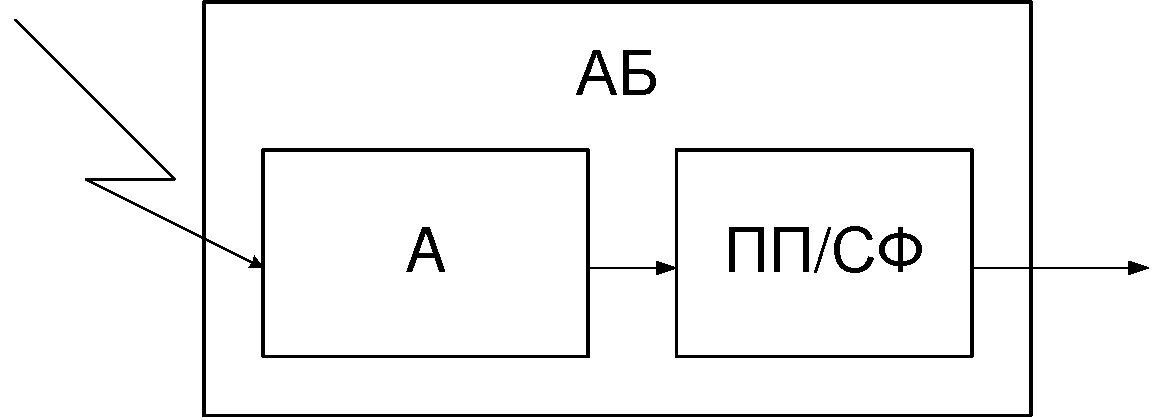
\includegraphics[scale=0.4]{ant_sns}
\caption{Схема антенного блоку СНС}
\label{fig:ant_sns}
\end{figure} 

Прийомообчислювач виконаний у вигляді блоку, у якому розташовані модулі вторинних 
джерел живлення і плати --- прийомокорелятора, навігаційного обчислювача та інтерфейсного 
пристрою (рис. \ref{fig:sns}). Вхід ПО через фідерну лінію з'єднаний з виходом антенного блоку. 
В аналоговому приймачі АП сигнали підсилюються, фільтруються і переносяться з несучої 
частоти на проміжну (зниження частоти). В аналого-цифровому перетворювачі АЦП аналоговий 
сигнал перетвориться в цифрову форму.
\begin{figure}[here]
\centering
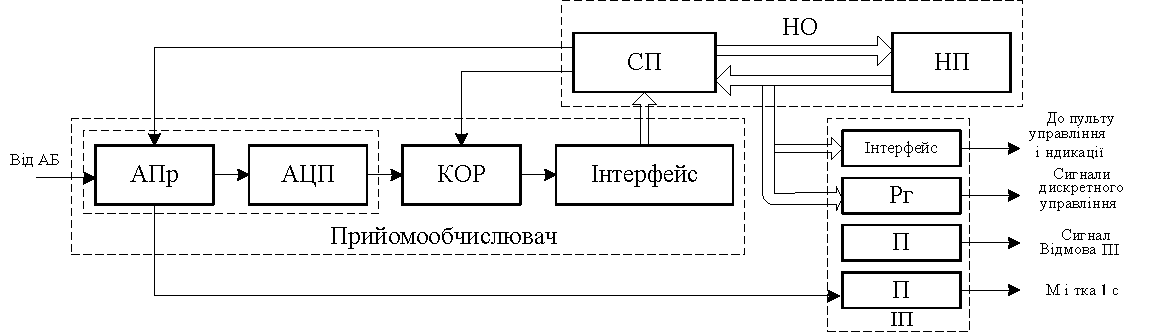
\includegraphics[scale=0.9]{sns}
\caption{Схема прийомообчислювача}
\label{fig:sns}
\end{figure} 
В кореляторі (КОР) у цифровій формі формуються синфазні  і квадратурні  відліки, що є 
основою роботи алгоритмів пошуку сигналів по затримці і частоті спостереження за псевдодальністю, 
фазою сигналу і виділення навігаційного повідомлення.

Навігаційний обчислювач НО є цифровим процесором, у якому реалізується обчислювальний процес 
і керування роботою ПІ. Навігаційний обчислювач зручно представити у виді сигнального процесора 
СП, що реалізує алгоритми первинної обробки квадратурних складових, і навігаційного процесора 
НП, що реалізує алгоритми низькочастотної обробки, тобто рішення навігаційної задачі.

У прийнятого радіосигналу виміряються затримка $\tau$ або доплерівський зсув частоти $f_{\text{доп}}$, 
які є радіонавігаційними параметрами, а відповідні їм дальність до об'єкта $D=c*\tau$  
і радіальна швидкість зближення $V_{p}=f_{\text{доп}}\lambda$   служать навігаційними параметрами 
(\textit{с } -- швидкість світла;$\lambda$ -- довжина хвилі радіосигналу).

Просторове положення споживача визначається в прийомоіндикаторі в два етапи: спочатку визначаються 
поточні координати супутників і первинні навігаційні параметри (дальність, її похідні й ін.) щодо 
відповідних НС, а потім розраховуються вторинні --- географічна широта, довгота, висота споживача і т.д.

Вектор швидкості споживача обчислюють шляхом обробки результатів вимірів доплерівських зсувів 
частоти сигналів НС з урахуванням відомого вектора швидкості супутника. 

Інтерфейсний пристрій (ІП) призначений для забезпечення взаємодії прийомоіндикатора з зовнішніми 
пристроями такими, наприклад, як пульт керування й індикації (ПКІ). Додатково до складу ІП входять 
два підсилювачі П, що формують ознаку відмови ПІ і сигнали дискретного керування, а також 8-розрядний 
регістр Рг, що приймає сигнали дискретного керування. Цей регістр доступний для читання з боку НО. 
Останній, у залежності від інформації, що знаходиться в регістрі, вибирає той або інший режим роботи.

Таким чином, основною операцією, що виконуваної в СНС за допомогою космічного сегменту, сегменту 
керування та сегменту споживача, є визначення просторових координат місця розташування споживачів і 
часу, тобто просторово-тимчасових координат (ПТК). Як було показано, цю операцію здійснюють відповідно 
до концепції незалежної навігації, що передбачає обчислення шуканих навігаційних параметрів 
безпосередньо в апаратурі споживача. У рамках цієї концепції в СРНС обраний позиційний спосіб 
визначення місця розташування споживачів на основі беззапитних (пасивних) далекомірних вимірів по 
сигналах декількох навігаційних штучних супутників Землі з відомими координатами. Висока точність 
визначення місця розташування споживачів обумовлена багатьма факторами, включаючи взаємне розташування 
супутників і параметри їхніх навігаційних сигналів. Структура космічного сегмента забезпечує для 
споживача постійну видимість необхідного числа супутників.

Використання СНС в інтересах місцезнаходження і навігації рухливих об'єктів, а також у рішенні 
спеціальних задач (спостереження, аерофотознімання, пошук корисних копалин, пошук і порятунок 
транспортних засобів, що терплять нещастя, і людей) висуває високі вимоги.

Вимоги до точнісних характеристик, таких як середньоквадратичне відхилення помилки (СКП) визначення 
навігаційних параметрів, показників надійності навігаційного забезпечення, тощо наступні:
\begin{itemize}
  \itemдоступність (готовність),  мірою якої є імовірність працездатності СРНС перед виконанням 
тієї або іншої задачі та у процесі її виконання. Чисельні значення доступності складають 0,95...\dots 0,997;
 \itemцілісність, мірою якої є імовірність виявлення відмови протягом часу, рівному заданому 
або менше. Вимоги до цілісності для маршрутних польотів складає 0,999;
 \itemбезперервність обслуговування, мірою якої служить імовірність працездатності системи 
протягом найбільш відповідальних відрізків часу. На етапах заходу на посадку вимоги до безперервності 
обслуговування складають $10^{-5}$ \dots ... $10^{-4}$ для проміжків часу від 15 до 150 с.
\end{itemize}

Основні навігаційні параметри, що визначаються в СРНС -- дальність і радіальна швидкість. Відповідними 
їм радіонавігаційними параметрами (параметрами радіосигналу) служать затримка t сигналу і доплерівський 
зсув частоти $f_\text{доп}$. Оскільки головною вимогою до СРНС є висока точність виміру 
навігаційних параметрів, отже, й основною вимогою до радіосигналів так само є висока точність 
виміру затримки t сигналу і доплерівського зсуву частоти $f_\text{доп}$.

Вимоги до підвищення точності затримки сигналу і доплерівського зсуву частоти суперечливі. 
Для підвищення точності виміру затримки необхідно розширювати спектр сигналу, а для підвищення 
точності виміру  доплерівського зсуву частоти --  збільшувати тривалість сигналу.

Дане протиріччя вирішується при вирішенні задачі спільної оцінки t та  $f_\text{доп}$.

Підвищення точності спільних оцінок затримки сигналу і доплерівського зсуву частоти можна 
досягти за рахунок збільшення так званої  бази сигналу -- \textit{В}(добуток ефективної 
тривалості сигналу на ефективну ширину спектра сигналу) і основною вимогою до радіосигналів у 
СРНС є збільшення бази сигналу $В>>1$. Такі сигнали називають шумоподібними. 
Відомо, що стійкість до перешкод радіотехнічної системи визначається значенням бази сигналу, 
а для більшості ЛА скритність і перешкодозахищеність є одним з визначальних вимог. 

Інша істотна вимога --- забезпечення багатостанційного доступу. При визначенні навігаційних 
параметрів у споживача повинна бути можливість одночасного доступу до сигналів від різних 
супутників. Проблема багатостанційного доступу вирішується шляхом тимчасового, частотного 
або кодового поділу сигналів, наприклад, у супутниковій навігаційній системі GPS використовується 
кодовий поділ, у СРНС ГЛОНАСС - частотний.

З результатів аналізів стає очевидно, що не має принципової різниці між супутниковими 
навігаційними системами GPS та ГЛОНАСС.

В залежності від області використання апаратура споживача (АС) має свої особливості, 
тому виробники АС завжди вказують на область застосування відповідного зразка. Крім 
основних блоків, таких, як антена, приймач, індикатор, АС може містити допоміжні, що 
забезпечують виконання спеціальних сервісних функцій, наприклад, діагностику вузлів 
транспортного засобу, зв'язок з диспетчерським пунктом і т.п.

В табл. \ref{tb:ac} наведені коротка інформація про основні зразки АС, що працюють за сигналами 
СРНС ГЛОНАСС та GPS. Наведена інформація не претендує на повноту відомостей як про існуючі 
зразки АС, так і про іх характеристики, а дається для ілюстрації досягнутого рівня 
в розробці та виробництві АС СРНС.
Апаратура споживачів
\begin{table}[here]
\small
\caption{Апаратура споживачів}
\centering
\begin{tabular}{|p{30mm}|p{20mm}|p{20mm}|p{20mm}|p{20mm}|p{20mm}|p{10mm}|} \hline 
Найменування апаратури & Область використання & Виробник & Число каналів & 
\multicolumn{2}{|p{30mm}|}{Точність (в автономному режимі)} & Маса, кг \\ \hline 
 &  &  &  & координат, м & швидкості, м/с &  \\ \hline 
Станція моніторингу та формування ДП & Моніторинг & РНИИ КЛ & 24 & 1...3 & 1...2 & 6,0 \\ \hline 
„Гном-М'' & Авіація &  & 6...12 & 80...90 & 12...15 & 3,2 \\ \hline 
АСН-22 & Авіація & РИРВ & 18 & 25...30 &  & 0,4 \\ \hline 
НАВИС СН 3301 & Авіація &  & 14 & 15...20 & 8...10 & 2,4 \\ \hline 
„Интер-А'' & Авіація & МКБ КОМПАС & 12 & 25...30 & 10...30 & 3,5 \\ \hline 
А-744 & Авіація & Фирма „Кодтик'' & 6 & 30...35 & 15...20 & 2,0 \\ \hline 
\end{tabular}
\label{tb:ac}
\end{table}

З огляду на, те що  супутникова система навігації буде працювати в комплексі з 
інерціальною системою навігації, то навряд варто встановлювати  на борт ЛА повний 
комплект супутникової системи. Досить обмежитися  прийомоіндикатором і сигнальним 
процесором, думаючи, що алгоритми рішення навігаційної задачі будуть вирішуватися 
в спільному процесорі інерціально - супутникової системи навігації. 

Виходячи з вищенаведеного, а також враховуючи умови застосування ЛА та вимоги 
ТЗ можна сформулювати вимоги, яким повинний задовольняти обраний тип прийомоіндикатора 
СРНС. 

Розв'язувані задачі:
\begin{itemize}
\item автоматичне, безперервне, глобальне, всепогодне визначення поточних ЗD-координат 
місця розташування, вектора шляхової швидкості шляхового кута ЛА при роботі: по 
сигналу стандартної точності частотного діапазону L1 ГЛОНАСС; по сигналі З/А-коду 
GPS; при спільній обробці вищевказаних сигналів;
\item видача поточних ЗD-координат місця розташування ЛА, що є складовими вектора 
швидкості і шляхового кута в системі координат СК-42 або ПЗ-90 у географічному 
форматі, а також ознак режиму роботи апаратури;
\item стійке визначення навігаційних параметрів при русі з лінійними прискореннями 
і при стрибкоподібних змінах прискорення;
\item  можливість переключення з антени носія на антену ЛА; 
\item інтегральна оцінка очікуваної точності визначення поточних координат місця розташування;
\item автоматичний вибір оптимального з погляду очікуваної точності сузір'я НС ГЛОНАСС і GPS при роботі в сполученому режимі;
\item автоматичне рішення навігаційної задачі в географічній системі координат:  
\end{itemize}

% Chapter 2 with subsections
\newpage
\ESKDthisStyle{formII}
\section{Аналіз та вибір методів оцінювання та корекції в комплексній інерціально-супутниковій системі}

Основними задачами пілотажно-навігаційних комплексів (ПНК) як постачальника 
інформаційного забезпечення польоту ЛА є сумісна обробка навігаційної інформації, 
яка надходить на борт ЛА та забезпечення високої надійності функціонування бортових 
систем та комплексів ЛА і взагалі безпеки польоту за рахунок резервування 
джерел інформації. Висока ефективність використання інформації, яка 
надходить на борт ЛА, забезпечується застосуванням різних методів її обробки. 

Найкращі результати підвищення якісних характеристик вимірювальних комплексів 
досягаються  в системах зі структурною надмірністю, коли існує можливість 
отримання пілотажно-навігаційної інформації паралельно декількома способами з 
використанням інформації від приладів та вимірювальних систем, що входять до 
складу ПНК. Отримана таким чином інформація комплексується.

В існуючих ПНК широке розповсюдження знайшли такі способи сумісної обробки 
інформації, що надходять від декількох вимірників, як взаємна компенсація і 
фільтрація похибок вимірювальних приладів, що вимірюють один і той самий 
навігаційний параметр та оптимальне оцінювання вектора стану з використанням 
апріорної інформації про контрольований процес та поточні вимірювання.

Методи оптимальної обробки інформації в ПНК використовуються з метою 
отримання оцінок вектора стану повітряного судна (або деякої частини 
цього вектора) в умовах впливу випадкових збурень і завад на процес 
вимірювання. При цьому оцінюються не самі параметри польоту, а їхні похибки. 
За оптимальної обробки пілотажно - навігаційної інформації в ПНК найважливішим 
процесом є процес отримання оптимальних оцінок. В основу алгоритмів отримання 
оптимальних оцінок можуть бути покладені такі методи обробки інформації:
\begin{itemize}
 \item метод найменших квадратів;
 \item метод максимуму правдоподібності;
 \item рекурентний неоптимальний фільтр;
 \item оптимальний фільтр Калмена.
\end{itemize}


\subsection{Рекурентний фільтр Калмана}

Термін оптимальна фільтрація відносять до методики оцінки стану динамічної системи, з якої ми 
спостерігаємо непрямі вимірювання. Стан відносить до фізичного стану, який може бути описаний 
динамічними змінними, такими як позиція, швидкість та прискорення рухомого об'єкту. Шум в вимірах 
означає, що  існує деяка  степінь невизначеності в них. Динамічна система залучає функції часу, 
а також шум в динаміці системи,  система не може бути змодельована як повністю детерміністичний 
процес. З цього боку, термін фільтрація  означає фільтрацію шуму в вимірах і забезпечення 
оптимального оцінювання змінних стану системи по відповідним вимірам і висунути припущення 
щодо динаміки системи.

Оптимальний фільтр Калмана \cite{bib:kalman_1} — ефективна і гнучка процедура для об'єднання інформації із зашумлених 
датчиків для оцінки стану стохастичної системии.
Фільтра включає 2 типа змінних:
\begin{enumerate}
 \item Вектор стану системи, включає наступні компоненти:
  \begin{itemize}
    \item Змінні, які безпосередньо нас цікавлять (необхідно знайти, наприклад швидкість, прискорення)
    \item Змінні, які безпосередньо не використовуються, але необхідні для процесу оцінювання. 
    В загальному випадку не важливо знати їхні значення, але необхідно визначити їх для для 
    покращення точності оцікни.
    \item Фільтр Калмана у специфічних задача має включати всі ті змінні динаміки системи, які можуть 
    бути виміряні ДПІ.
    \end{itemize}
 \item Коваріаційна матриця: міра невизначеності оцінювання. Рівняння, що використовуються для 
отримання коваріаційної матриці ( рівняння Рікатті) та управління невизначеністю, визначають 
як шум датчиків та динаміка невизначеності впливають на невизначеність стану системи, що оцінюється.
\end{enumerate}

За допомогою отримання невизначеності власне системи і невизначеності у відповідних 
показника датчиків, ФК дає можливість комплексувати данні з усіх ДПІ “отимально”, в 
сенсі, що результуюча оцінка мінімізує квадратичну функцію помилки оцінки, включаючи 
мінімальне середньо квадратичне відхилення будь-якої лінійної комбінації помилок оцінювання. 
Коефіцієнт підсилення Калмана — оптимальна зважена матриця, що поєднує данні ДПІ з попередньою 
оцінкою, для отримання нової апостеріорної оцінки.


\textbf{Рівняння динамічної системи}

Фільтр Калмана намагається оцінити стан змінної $x\in \Re^{n}$ дискретно управляємий
процес, що описується лінійним стохастичним диференціальним рівнянням
\begin{equation}
\label{eq:linear_sys}
x_{k} = \Phi x_{k-1} + w_{k-1},
\end{equation}
З вимірюваннями  $Z\in \Re^{m}$:
\begin{equation}
\label{eq:linear_sys_measure}
z_{k} = Hx_{k} +v_{k},
\end{equation}

Випадкові змінні $w_{k}$ та $v_{k}$ представляють шум системи (process noise) та 
шум вимірювань (measurement noise), які вважаються незалежними один від одного,
білими з нормальним розподілом шумами.
\begin{equation}\label{eq:pw} p(w)\sim N(0,Q),\end{equation}
\begin{equation}\label{eq:pv} p(v)\sim N(0,R).\end{equation}

На практиці, коваріаційна матриця шуму системи \textbf{Q} та коваріаційна
матриця шуму вимірювань \textbf{R} можуть змінюватись на кожному кроці вимірювань,
але для простоти в нашому випадку вони постійні.

Матриця $\Phi$ розміром $n \times n$ в диференціальному рівнянні \eqref{eq:linear_sys}
проводить залежність між попереднім станом системи $k-1$ та поточним станом
$k$, при наявності вхідного сигналу чи шуму. Матриця \textbf(H) $m \times n$ в 
рівнянні \eqref{eq:linear_sys_measure} відповідає вимірюванням $z_{k}$. 

\textbf{Отримання рівнянь фільтра}

Позначимо $\hat{x}(-) \in \Re^{n}$ --- апріорна оцінка на кроці $k$ 
інформація про рух системи до кроку $k$, та $\hat{x}(+) \in \Re^{n}$
апостеріорна оцінка на кроці $k$ за допомогою вимірювань $z_{k}$. 
Відповідно апріорна оцінка коваріації помилки:
\begin{equation}
\label{eq:p_minux}
P_{k}(-)= E[(x_{k}-\hat{x}_{k}(-))(x_{k}-\hat{x}_{k}(-))_{T}]
\end{equation}
та апостеріорна коваріаційна матриця помилок:
\begin{equation}
\label{eq:p_plus}
P_{k}(+)= E[(x_{k}-\hat{x}_{k}(+))(x_{k}-\hat{x}_{k}(+))_{T}]
\end{equation}

При виведенні рівнянь фільтра Калмана, наша ціль -- знайти рівняння, що 
розраховують апостеріорну оцінку стану $\hat{x}_{k}(+)$ як лінійна компенсація
апріорної оцінки стану $\hat{x}_{k}(-)$ та взваженої різниці між безпосередньо
вимірами $z_{k}$ та їх прогнозом $H\hat{x_{k}}$, як показано нижче \eqref{eq:k_update}
\begin{equation}
  \label{eq:k_update}
 \hat{x}_{k}(+)= \hat{x}_{k}(-) + K\left(z_{k}-H\hat{x}_{k}(-)\right)
\end{equation}
Різниця $(z_{k}-H\hat{x}_{k}(-))$  -- називається інноваціями (innovation) 
або залишками (residual). Залишки, як відображення дисперсії між прогнозованими
вимірами $H\hat{x}_{k}(-))$ та безпосередніми вимірами $z_{k}$. Залишок, який
рівний нулю, означає, що обоє вимірів знаходяться в повному узгодженні.

Матриця \textbf{K} $n \times m$ визначає коефіцієнт підсилення або фактор
змішування, який мінімізує апостеріорну помилку оцінки \eqref{eq:p_plus}.
Мінімізація може бути закінчена підстановкою \eqref{eq:k_update} у подане 
вище визначення для коваріації \eqref{eq:p_plus}, виконуючи необхідні дії та
взявши похідну по \textbf{K}, встановивши результат рівним нулю, а потім
вирішуючи відносно \textbf{K} рівняння. Результат може бути отриманий в 
наступній формі:
\begin{equation}
  \label{eq:k_gain}
  K_{k}=P_{k}(-)H^{T}(HP_{k}(-)H^{T}+R)^{-1} = \frac{P_{k}(-)H^{T}}{HP_{k}(-)H^{T}+R} 
\end{equation}
Зважаючи на \eqref{eq:k_gain}, якщо коваріаційна матриця помилок вимірювання
\textbf{R} прямує до нуля, коефіцієнт підсилення \textbf{K} взважує залишки 
більш сильно.Наприклад:
\begin{equation}
  \label{eq:lim_R}
  \displaystyle\lim_{R_{k}\to 0} K_{k} = H^{-1}
\end{equation}
Якщо апріорна оцінка коваріаційної матриці $P_{k}(-)$ наближається
до нуля, коефіцієнт підсилення \textbf{K} майже не взважує залишки.
\begin{equation}
  \label{eq:lim_P_minus}
  \displaystyle\lim_{P_{k}(-)\to 0} K_{k} = 0
\end{equation}

З іншого боку, взважування за допомогою \textbf{K}, у випадку коли коваріація 
помилки вимірювань \textbf{R} наближається до нуля, то безпосереднім вимірам
$z_{k}$ довіряється все більше і більш, коли прогнозовані виміри $H\hat{x}_{k}(-))$
враховуються все менше. Але якщо апріорна коваріація помилки $P_{k}(-)$ наближається
до нуля то спостерігання $z_{k}$ майже не враховуються, коли відповідно
прогнозовані виміри $H\hat{x}_{k}(-))$ стають більш ``впливовими''.


\subsection{Алгоритм фільтра Калмана}

ФК знаходить стан системи за допомогою форми зворотнього зв'язку: фільтр
оцінює стан процесу в один момент часу, а потім отримує зв'язок в формі
зашумлених вимірів. Такі рівняння для фільтра розділяються на дві групи: 
прогноз та корекція на основі вимірів. Прогноз відповідає за екстраполяцію
в часі поточного стану системи та її коваріації для отримання апріорної
оцінки для наступного кроку. Рівняння корекції необхідні для зворотнього
зв'язку -- використовують нові виміри і апріорні оцінки для отримання 
апостеріорних оцінок.

Для фільтра не важливо з якого кроку починати, так і рівняння можуть бути 
представлені з точки зору прогнозу та корекції Рис.\ref{fig:basic_cycle}
\begin{figure}[here]
\centering
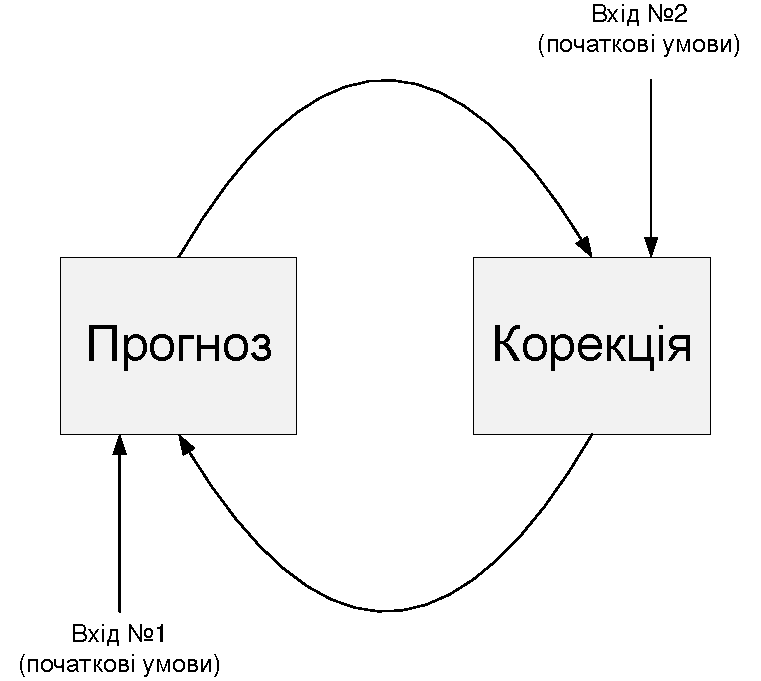
\includegraphics[scale=0.55]{pre_upd}
\caption{Цикл функціонування фільтра Калмана }
\label{fig:basic_cycle}
\end{figure} 



\begin{table}[here]
\small
\caption{Рівняння дискретного фільтра Калмана}
\centering
\begin{tabular}{|p{160mm}|} \hline 


Рівняння / Формула \\ \hline 
\begin{eqnarray} 
% \begin{array}{cc}
\text{Модель динаміки системи}  &  \label{eq:kalman_1} x_{k} = \Phi x_{k-1} + w_{k-1}, \\  
\text{Модель вимірювань}  & \label{eq:kalman_2} z_{k} = Hx_{k} +v_{k} \\ 
\text{Початкові умови}  &\label{eq:kalman_3} E[x_{o}] = \hat{x}_{0}, E[x_{o} x_{o}^{T}] = P_{0} \\
\text{Припущення незалежності}  &  \label{eq:kalman_4} E[w_{k} v_{j}^{T}] = 0 \text{для всіх k та j} \\
\text{Екстраполяція оцінки (прогноз)}  &  \label{eq:kalman_5} \hat{x}_{k}(-) = \Phi \hat{x}_{k-1}(+)\\
\text{Екстраполяція коваріації}  &  \label{eq:kalman_6} P_{k}(-) = \Phi_{k-1} P_{k-1}(+)\Phi_{k-1}^{T} + Q_{k-1} \\ 
\text{Корекція оцінки}  &  \label{eq:kalman_7} \hat{x}_{k}(+) = \hat{x}_{k}(-) + K_{k}[z_{k}-H_{k}\hat{x}_{k}(-)]\\
\text{Корекція оцінки коваріації}  &  \label{eq:kalman_8} P_{k}(+) = [I - K_{k}H_{k}]P_{k}(-)\\
\text{Коефіцієнт підсилення Калмана}   &  \label{eq:kalman_9} K_{k}= P_{k}(-)H_{k}^{T}[H_{k}P_{k}(-)H_{k}^{T} + R_{k}]^{-1}  
% \end{array}
\end{eqnarray} 
\\  \hline
\end{tabular}
\label{tb:ac}
\end{table}
Перше завдання при корекції -- розрахувати коефіцієнт підсилення Калмана, $K_{k}$/
Наступний крок, безпосередньо отримати виміри $z_{k}$, а потім генерувати 
апостеріорну оцінку за допомогою \eqref{eq:k_update}. Останній крок  -- це 
отримання апостеріорної коваріаційної матриці оцінки помилки.

Після кожного разу екстраполяції та корекції, процес повторюється, попередні
апостеріорні оцінки використовуються для прогнозу нових апріорних оцінок.
Ця рекурсивна природа є найбільш важливою особливістю фільтра Калмана, це робить
його більш практичним, в порівнянні з іншими фільтрами (наприклад фільтр Віннера)
\begin{figure}[here]
\centering
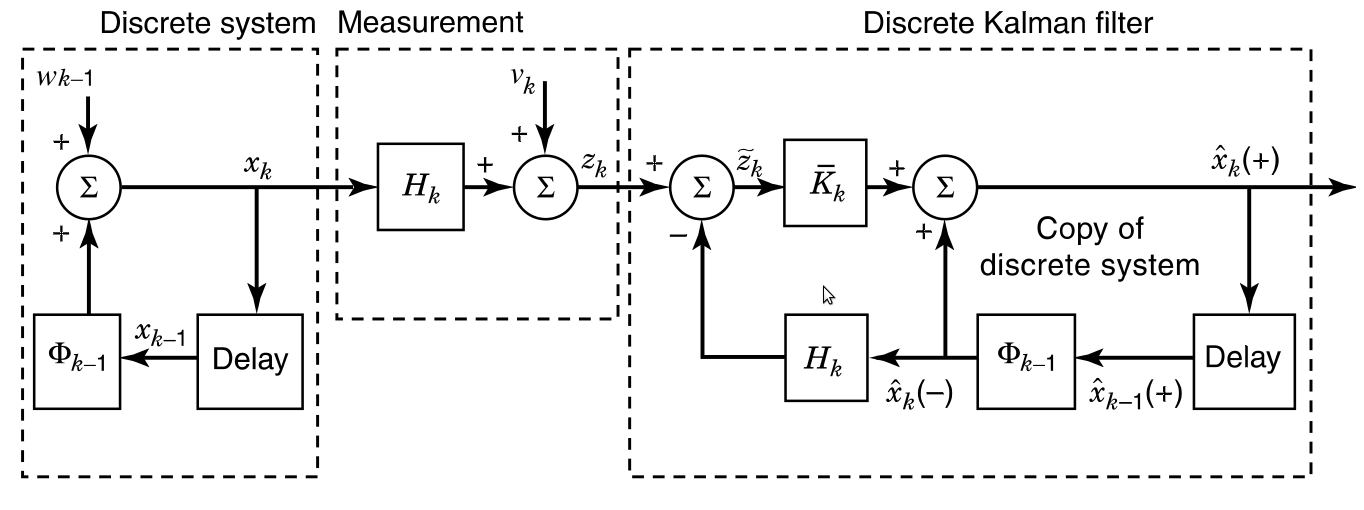
\includegraphics[scale=0.35]{kalman_flow}
\caption{Блок діаграма системи, моделі вимірювань та дискретного ФК}
\label{fig:kalman_flow}
\end{figure} 

\subsection{Проектування фільтра Калмана}

В практичній реалізації фільтра, коваріація вимірюваного шуму R вимірюється
звичайно до використання фільтра. Знаходження цієї матриці в загальному випадку
практична задача, виміряні величини дають можливість визначити дисперсію шуму, що
діє на данні датчиків.

Визначення коваріації шуму системи Q в загальному більш складна задача,
просто не має можливості безпосередньо спостерігати процес який оцінюється.
Інколи відносно проста модель процесу може дати прийнятний результат, якщо
введена достатня величина невизначеності процесу через вибір матриці Q.

В іншому випадку, є чи немає раціональної бази для вибору параметрів, часто
краща продуктивність (з точки зору статистики) може бути отримана за допомогою
налаштування параметрів фільтра Q та R. 

Асиметрія коваріаційної матриці $P$ один з факторів, що впливає на чисельну
нестійкість рівняння Рікатті. Якщо не використовується фільтр з квадратним
коренем, тоді ця матриця може бути ``симетризована'' просто за наступною 
формулою:
\begin{equation}
 \label{P_symetry}
P= \frac{1}{2}(P+P^{T})
\end{equation}
Цей метод використовується протягом довгого часу і добре себе зарекомендував.

При проектуванні фільтра, корекція коваріаційної матриці \eqref{eq:kalman_6} та
\eqref{eq:kalman_8} має бути перевірена не тільки на симетрію але й на 
додатно визначеність.
Якщо ці умови не будуть виконуються, це свідчить про помилки в програмі або
матриця погано обумовлена. Для усунення проблеми обумовленості використовується
інше рівняння для $P_{k}(+)$, яке називається формою Джозефа \cite{joseph}, яка показна на
наступному рівнянні:
\begin{equation}
 \label{P_plus_Joseph}
P_{k}(+)=[I-K_{k}H_{k}]P_{k}(-)[I-K_{k}H_{k}]^{T}+K_{k}R_{k}K_{k}^{T}
\end{equation}
З рівняння видно, що права частина є сумою двох симетричних матриць.
Перша додатно визначена інша не від'ємно визначена, що робить $P_{k}(+)$ 
додатно визначеною матрицею.

Безперечно саме фільтр Калмана найбільш привабливий при розв’язанні задачі 
комплексної обробки інформації в інерціально-супутникових системах навігації. 
Проте використання фільтра Калмана зустрічає певні труднощі при його практичної
 реалізації на борту ЛА. Зокрема в жорстко зв’язаних   інерціально-супутникових 
системах навігації,  фільтр Калмана повинний бути дуже швидкодіючим, що обмежується 
характеристиками існуючих процесорів бортових ЦОМ. 





\ESKDthisStyle{formIIab}
\subsection{Алгоритми роботи трикомпонентної БІНС}

Алгоритм функціонування БІНС містить у собі сукупність аналітичних залежностей, які 
дозволяють за вимірюваним значенням уявного прискорення й абсолютної кутової швидкості 
ЛА безперервно визначати поточне значення координат місця розташування, складові 
шляхової швидкості та кутове положення ЛА в обраній навігаційній системі координат.

В алгоритмах роботи  трикомпонентної БІНС, як і в алгоритмах платформної ІНС, точність 
зчислення навігаційних параметрів досягається за рахунок виключення із сигналів уявного 
прискорення, яке вимірюють акселерометри, складові прискорення сили ваги і коріолісового 
прискорення. Але вплив цих складових компенсується на відміну від платформної ІНС 
тільки аналітично. 

Кінематичні рівняння інерціальної  навігації в основному визначаються вибраною системою 
координат, тобто навігаційним базисом, в якому визначаються навігаційні параметри 
(координати і проекції швидкості). У свою чергу, вибір навігаційного базису залежить 
від типу літального апарата, особливостей його траєкторного руху, характеру розв'язуваних 
задач.

Наприклад, для БІНС, що інтегруються зі супутниковими навігаційними системами, можна 
застосовувати інерціальну систему координат, яка використовується супутниковою системою 
навігації.  При цьому, позиційну інформацію одержують у формі декартових прямокутних 
координат, швидкісну -- у формі проекцій абсолютної швидкості на осі вибраної інерціальної 
системи координат, а інформацію про кутову орієнтацію -- у вигляді відповідної матриці 
або трьох кутів орієнтації ЛА відносно вибраного базису. Подальше перерахування отриманих 
координат в обертову систему координат ПЗ-90 (WGS-84) здійснюється за алгоритмами 
супутникової системи навігації.

Для БІНС літальних апаратів, які здійснюють рух в атмосфері Землі, найбільш часто 
використовуються обертові системи координат з базовою площиною місцевого горизонту 
і певною орієнтацією горизонтальних осей в азимуті. Під орієнтацією осей в азимуті 
розуміється можливість їхньої орієнтації, наприклад, за сторонами світу, коли дві 
горизонтальні осі спрямовані в східному і північному напрямках. При цьому позиційну 
інформацію визначають широтою $\varphi$, довготою $\lambda$ і висотою \textit{h}, 
що виміряні на еліпсоїді Красовського або на еліпсоїді міжнародної системи WGS-84, 
швидкість визначають проекціями на східну $V_E$, північну $V_N$ і вертикальну 
осі $V_H$, якщо за навігаційну систему вибрана система з орієнтацією осей за 
сторонами світу, або проекціями на осі горизонтального базису з іншою орієнтацією. 
Орієнтація при цьому визначається кутами крену, тангажа і аправжнього курсу.

Типову схему побудови БІНС зображено на рис. \ref{fig:SDINS}. Цей варіант реалізує алгоритм системи, 
яка працює в обертовій земній системі координат.

Датчики первинної інформації БІНС -- датчики кутової швидкості й акселерометри встановлюються 
жорстко на ЛА. Складні умови роботи датчиків інформації призводять до появи значних 
похибок, тому в алгоритмах роботи БІНС бажано здійснити аналітичну компенсацію похибок 
вимірників (здійснювати їх польотне калібрування), перш ніж ці сигнали будуть використані 
для розрахунку параметрів орієнтації і для визначення складових уявного прискорення 
уздовж навігаційних осей.

Для корекції показань датчиків первинної інформації необхідна математична модель 
вимірника, в якій, зазвичай, враховують: нелінійність; неспіввісність осей датчиків; 
дрейф; викривлення масштабного коефіцієнта.

\begin{figure}[here]
\centering
%\includegraphics[scale=0.9]{earth}
\caption{Алгоритм роботи БІНС}
\label{fig:SDINS}
\end{figure} 

Сигнали $\omega_{x,y,z}$ з виходу аналітичного компенсатора похибок використовуються 
для обчислення параметрів матриці напрямних  косинусів \textit{В}, яка визначає зв'язок 
між двома системами координат. Оскільки матриця напрямних  косинусів \textit{В} визначається 
між зв'язаними з ЛА осями й осями обертової навігаційної системи координат, то при 
розрахунках параметрів матриці \textit{В }необхідно залучити обчислені проекції вектора 
кутової швидкості навігаційної системи координат, що відображено на схемі додатковими 
зв'язками, які враховують кутову швидкість, що виникає при обльоті сферичної Землі $(
\dot{\lambda },\, \dot{h},\, \dot{\varphi })$, і кутову швидкість обертання самої 
Землі $(\Omega_{\text{З}} )$.

Перетворення складових уявного прискорення $a_{x,y,z}$  від осей ЛА до осей навігаційної 
системи координат здійснюється за допомогою матриці напрямних  косинусів \textit{В}. Навігаційний 
обчислювач вирішує задачі, властиві всім платформним системам, оскільки на вході 
цього обчислювача сформовані проекції уявного прискорення на осі навігаційної системи 
координат і нічого принципово нового в розв'язанні цієї задачі немає. На виході БІНС 
формуються радіус-вектор місця розташування ЛА, вектор швидкості, а також кути орієнтації 
ЛА. 

В окремому випадку, коли за навігаційний базис вибраний горизонтальний орієнтований 
за сторонами світу тригранник, на виході системи будуть сформовані географічні (геодезичні) 
координати радіуса-вектора місця розташування $\lambda$, $\varphi$, \textit{H}, проекції 
відносної швидкості руху $V_N$, $V_E$, $V_H$, а також 
кути орієнтації ЛА в географічній системі координат -- справжній курс $\psi$, тангаж $\vartheta$ і 
крен $\gamma$. 

Обсяг обчислень у БІНС значний. Це пояснюється в основному тим фактом, що БЦОМ розв'язує 
задачі, які пов'язані з динамікою обертання ЛА, а також з динамікою поступального 
руху ЛА. Поступальні швидкості ЛА відносно малі. Наприклад, швидкість при польоті 
ЛА в напрямку на північ 1100 км/год відповідає швидкості зміни широти усього на 10 
град/год.

Таким чином, інтегрування для одержання швидкості і місця розташування можуть здійснюватися 
досить точно з використанням дуже простих методів чисельного інтегрування при низькій 
частоті повторення   в типовому випадку 10...20 Гц .

Кутові швидкості ЛА в типовому випадку за величиною на кілька порядків більші поступальних 
швидкостей. Зокрема, для маневрених ЛА кутові швидкості обертання можуть складати 
сотні градусів за секунду. В результаті цього інтегрування кутового положення в БІНС 
зв'язано з жорсткими вимогами до БЦОМ.

Оскільки для забезпечення високої точності інерціальної навігації потрібно, щоб похибки 
інтегрування кутового положення обмежувалися декількома частками кутової хвилини, 
необхідно застосовувати алгоритми інтегрування більш високого порядку при типових 
частотах повторення  80...50 Гц. 

З огляду на вище сказане, наведемо  варіант побудови алгоритмів БІНС для випадку, 
коли за навігаційний базис вибраний горизонтальний орієнтований за сторонами світу 
тригранник.
\vspace{5mm}

\textbf{Алгоритми БІНС, яка працює в географічній системі координат}

За навігаційний тригранник візьмемо тригранник \textit{NHE}, зв'язаний з земною поверхнею.
\begin{figure}[here]
\centering
%\includegraphics[scale=0.9]{earth}
\caption{Системи координат}
\label{fig:earth}
\end{figure} 
Виберемо наступний напрямок осей   \textit{NHE} (рис. \ref{fig:earth}):

\textit{OH } --збігається з вертикаллю;\\
\textit{ON} -- дотична до меридіана;\\
\textit{ОЕ} -- утворює праву трійку.\\ 

В алгоритмах БІНС, зазвичай, виділяють динамічні та кінематичні рівняння. 
Динамічні рівняння реалізують трикомпонентну схему БІНС, у якій географічні координати  $\lambda$, 
$\varphi$,\textit{Н} визначаються інтегруванням рівнянь вигляду

\[\begin{array}{l} 
{\dot{\lambda}=\frac{V_{E} }{(R_{2} +H)\cos \varphi} ;} \\ 
{\dot{\varphi}=\frac{V_{N} }{R_{1} +H} ;} \\ 
{\dot{H}=V_{H,} } 
\end{array}\] 

\begin{ESKDexplanation}
\item де  $V_{N}$,$V_{E}$ -- північна та східна проекції шляхової швидкості 
(проекції на осі  системи координат \textit{NHE}  (див. рис. \ref{fig:earth}); 
\item $R_1$, \textit{R}2 -- два радіуси кривизни земного сфероїда (еліпсоїда обертання); 
\item $R_1$ -- радіус кривизни меридіонального перетину еліпсоїда (площиною \textit{HN}); 
\item $R_2$  -- радіус кривизни перетину еліпсоїда площиною \textit{HЕ} (площиною першого вертикала); 
\end{ESKDexplanation}

\[
R_{1} =\frac{a(1-e^{2})}{(1-e^{2} \sin(\varphi)^{2})^{\frac{3}{2}} }; \,\\
R_{2} =\frac{a}{\sqrt{1-e^{2} \sin(\varphi)^{2} } }.
\] 

\begin{ESKDexplanation}
\item де\textit{ a}  --- велика піввісь  еліпсоїда (\textit{a }=  6378388 м); 
\item \textit{e} --- ексцентриситет еліпсоїда  ($e^{2} = 6,73 10^{-3}$);  
\item \textit{Н}  --- висота польоту. 
\end{ESKDexplanation}

Тут можна застосовувати такі ж спрощення, що й у платформних інерціальних системах. 
Зокрема, функції   $\frac{1}{R_{1} +H}$ та $\frac{1}{R_{2} +H} $ 
з точністю до членів порядку малості $10^{-5}$ можна представити 
в наступному вигляді:

\[\begin{array}{l} 
{\frac{1}{R_{1} +H} =\frac{1}{a} [1-e^{2} -\frac{H}{a} 
-\frac{3}{2} e^{2} \sin ^{2} \varphi-2e^{2} \frac{H}{a} +3e^{2} \frac{H}{a} \sin 
^{2} \varphi + (\frac{H}{a} )^{2} +}\\
{+e^{4} (1-3\sin ^{2} B+\frac{3}{8}\sin ^{4} \varphi);} \\ 

{\frac{1}{R_{2} +H} =\frac{1}{a}[1-\frac{H}{a} 
-\frac{1}{2} e^{2} \sin ^{2} \varphi+(\frac{H}{a})^{2} +e^{2} \frac{H}{a} 
\sin ^{2} \varphi+} \\ 
{+e^{4}(\frac{1}{4} \sin ^{2} \varphi-\frac{3}{8})\sin ^{2} \varphi]} 
\end{array}\] 

Якщо у формулах $\frac{1}{R_{1} +H}$ та $\frac{1}{R_{2} +H}$ 
зберегти лише члени порядку малості $10^{-2}$ , то вони приймуть 
вигляд

\begin{equation} 
\label{eq:elips} 
\begin{array}{l} 
{\frac{1}{R_{1} +H} \approx \frac{1}{a}[1-e^{2} -\frac{H}{a} -\frac{3}{2} e^{2} \sin(B)^{2}];} \\ 
{\frac{1}{R_{2} +H} \approx \frac{1}{a}[1-\frac{H}{a} -\frac{1}{2} e^{2} \sin(\varphi)^{2}].} 
\end{array} 
\end{equation} 

Слід відзначити, що використання спрощень \eqref{eq:elips} може призвести 
до похибок, порівняних з похибками високоякісних гіроскопічних вимірників, які використовуються 
в БІНС.

Складові шляхової швидкості ЛА  $V_E$ , $V_N$ , $V_H$  одержують в результаті інтегрування 
проекцій сигналів акселерометрів, виключаючи із них  складові коріолісового прискорення  і 
прискорення сили ваги: 

\begin{equation} 
\label{eq:Vi} 
 \begin{array}{l} 
{\dot{V}_{E} =a_{E} -(V_{N} \omega_{H_{\Sigma } } -V_{H} \omega_{N_{\Sigma} } )+g_{E} ;} \\ 
{\dot{V}_{H} =a_{H} -(V_{E} \omega_{N_{\Sigma } } -V_{N} \omega_{E_{\Sigma} } )+g_{H} ;} \\ 
{\dot{V}_{N} =a_{N} -(V_{H} \omega_{E_{\Sigma } } -V_{E} \omega_{H_{\Sigma} } )+g_{N} ,} 
\end{array}
\end{equation} 
\begin{ESKDexplanation}
\item де $a_{E,H,N} $ -- проекції уявного прискорення ЛА, вимірювані акселерометрами, 
на осі навігаційного тригранника; 
\item $g_{E,H,N} $ --- проекції вектора прискорення 
сили ваги, які враховують прискорення земного тяжіння, і прискорення, що викликається 
відцентровою силою інерції і зв'язане з обертанням Землі; 
\item складові в дужках --- проекції коріолісового прискорення на осі навігаційного тригранника; 
\item $\omega_{E_{\Sigma}}\, \omega_{H_{\Sigma}}\, \omega_{N_{\Sigma}}$ --- проекції кутової 
швидкості навігаційного тригранника відносно інерціального простору, які враховують 
проекції кутової швидкості обертання Землі $\Omega_{E}$, $\Omega_{H}$, $\Omega_{N}$ 
і складові відносної кутової швидкості навігаційного тригранника, які обумовлені 
рухом ЛА відносно Землі $\omega_{E_{V} }$, $\omega_{H_{V} }$, $\omega_{N_{V}}$: 
\end{ESKDexplanation}

\[
\omega_{N_{\Sigma } } =\omega_{N_{V} } +2\Omega_{N} ;\\ 
\omega_{H_{\Sigma } } =\omega_{H_{V} } +2\Omega_{H} ;\\
\omega_{E_{\Sigma } } =\omega_{E_{V} } +2\Omega_{E} .
\] 

У свою чергу, складові відносної кутової швидкості навігаційного тригранника і швидкості 
обертання Землі визначаються співвідношеннями
\[
\begin{array}{l} 
{\omega_{E_{V}} =-\frac{V_{N} }{R_{1} +H} =-\dot{\varphi};} \\ 
{\omega_{H_{V}} =\frac{V_{E}}{(R_{2} +H)} tg\varphi=\dot{\lambda}\sin \varphi;} \\ 
{\omega_{N_{V}} =\frac{V_{E} }{(R_{2} +H)} =\dot{\lambda}\cos \varphi;} \end{array}\] 

\[
\Omega_{N} =\Omega_{\text{З}}\cos \varphi;
\Omega_{H} =\Omega_{\text{З}}\sin \varphi; 
\Omega_{E} =0,
\] 

\begin{ESKDexplanation}
 \item де  $\Omega_{\text{З}} $ --- кутова швидкість обертання Землі ($\Omega_{\text{З}}=7,27 \cdot 10^{-5}$ рад/с).
\end{ESKDexplanation}

Детермінована математична модель прискорення сили ваги існує тільки для нормальної 
складової поля сили ваги, що відповідає земному еліпсоїду з рівномірним розподілом 
мас в об'ємі цієї фігури. Градієнт цього поля в будь-якій точці, що належить поверхні 
еліпсоїда, спрямований за нормаллю до неї і розташований у площині меридіонального 
перетину. Оскільки точка місцеположення ЛА не належить поверхні Землі, то вектор 
градієнта нормального поля сили ваги $\bar{g}$ в цій точці не буде спрямований за 
лінією нормалі, опущеної з неї до поверхні земного еліпсоїда (вісь \textit{ОН}). 
Разом з тим, цей вектор буде розташований у площині меридіана точки \textit{О}, тобто 
в площині \textit{NOH. }Тоді, використовуючи  потенційну функцію нормального поля 
тяжіння земного сфероїда, з точністю до членів порядку малості $10^{-5}$  співвідношення 
для проекцій складових поля сили ваги $\bar{g}$ мають такий вигляд:
\[
\begin{array}{l} 
{g_{E} =0;} \\
{g_{N} =\frac{1}{2} g[\frac{H}{a} (e^{2} -5q)+qe^{2} \sin^{2}\varphi]\sin^2\varphi;}\\
{g_{H} =-g\left\{1-2\frac{H}{a} -\right. (e^{2} +2q-3\frac{H}{a})
\frac{H}{a} +\left[\frac{1}{2} (5q-e\right. ^{2} )-\frac{1}{8} e^{4} +\frac{17}{18}qe^{2} +} \\ 
{ +(3e^{2} - 5q)\frac{H}{a} ]\sin ^{2} B-\frac{1}{2} qe^{2} \sin ^{4} \varphi+\frac{1}{16} e^{2} 
(\frac{1}{2} e^{2} -7q)\sin ^{2} 2\varphi\},} 
\end{array}
\]
\begin{ESKDexplanation}
\item де \textit{g}= 9,78049 м/с2 прискорення сили ваги на екваторі; 
\item \textit{q} = $\Omega_{\text{З}}^{2} $ \textit{a/g} = 0,00346775 --- відношення 
відцентрової сили, обумовленої обертанням Землі, до сили ваги на екваторі. 
\end{ESKDexplanation}

З точністю до величин порядку малості $10^{-4}$ співвідношення для проекцій складових 
поля сили ваги $\bar{g}$ декілька спрощуються:

\[
\begin{array}{l} 
{ g_{E} =0;} \\ 
{g_{N} =g\sin 2\varphi+\frac{5}{2} q\sin ^{2} B\frac{H}{a}(\frac{e^{2} }{2} -2q);} \\ 
{g_{H} =-g\left[1-\frac{e^{2} }{2}\sin ^{2} \varphi+\frac{3}{2} q\sin ^{2} \varphi+e^{4}(-\frac{1}{8} \sin ^{2} \varphi+\frac{1}{32} 
\sin ^{2} 2\varphi\right)+} \\ 
{ +e^{2} q\left(-\frac{17}{28} 
\sin ^{2} \varphi-\frac{5}{16} \sin ^{2} 2\varphi\right)+\frac{H}{a} e^{2} (3\sin ^{2} \varphi-1)+}\\ 
{ +\frac{Hq}{a} (-1-6\sin ^{2}\varphi)-2\frac{H}{a} +3\frac{H^{2} }{a^{2} }],} 
\end{array}
\] 

а при малих значеннях висоти ($Н\leq$ 100 км ) проекції вектора  $\bar{g}$ на 
осі \textit{NHE}, якщо в них зберегти лише члени порядку малості $10^{-2}$, 
взагалі мають простий вигляд: 
\[
\begin{array}{l} 
{g_{E} =0;}\\
{g_{N} =0;}\\ 
{g_{H} =-g(1+5,2884\cdot 10^{-3} \sin ^{2}\varphi)[1-\frac{2H}{a}
(1-e\sin^{2}\varphi )]} 
\end{array}
\] 
Є й інші форми запису даної складової.

При розв'язанні кінематичних рівнянь розраховуються проекції $a_{E,H,N} $ уявного 
прискорення ЛА на осі навігаційного тригранника \textit{NHE}за показаннями акселерометрів 
зі зв'язаної з ЛА системи координат \textit{XYZ} з використанням матриці напрямних  
косинусів \textbf{В}

\[
 \left[\begin{array}{c} 
{a_{N} } \\ 
{a_{H} } \\ 
{a_{E} }
\end{array}\right]=B
\left[\begin{array}{c} 
{a_{x_{\text{ЛА}} } } \\ 
{a_{y_{\text{ЛА}} } } \\ 
{a_{z_{\text{ЛА}} } } 
\end{array}\right]
\] 

Матриця напрямних  косинусів  має такий вигляд:

\[
B=\left[\begin{array}{c|c|c} 
{\cos \psi \cos \vartheta } & 
{\sin \psi \sin \gamma -\cos \psi \sin \vartheta \cos \gamma } & 
{\sin \psi \cos \gamma +\sin \gamma \sin \vartheta \cos \psi } \\  \hline {\sin \vartheta } & 
{\cos \vartheta \cos \gamma} & 
{-\cos \vartheta \sin \gamma } \\  \hline {-\sin \psi \cos \vartheta } & 
{\cos \psi \sin \gamma +\sin \psi \sin \vartheta \cos \gamma } & 
{\cos \psi \cos \gamma -\sin \psi \sin \vartheta \sin \gamma } 
\end{array}\right]
\] 

де $\gamma$, $\vartheta$, $\psi$ -- кути крену, тангажа і рискання. Кут рискання 
відрізняється від географічного курсу $\psi$г знаком, тобто $\psi$г = $\psi$.

Матриця напрямних  косинусів \textbf{В} може бути отримана в різні способи. Наведемо приклади 
деяких з них. 

Знайти матрицю \textbf{В} можна в результаті розв'язання 
узагальненого рівняння Пуассона за інформацією про кутову швидкість ЛА відносно інерціального 
простору $\omega_{\text{ЛА}}$ і кутову швидкість навігаційної системи координат відносно 
інерціального простору $\omega_{NHE}$, яка враховує кутову швидкість 
обертання Землі і кутову швидкість, обумовлену обльотом ЛА сферичної Землі 

\[
  \dot{B}=B\omega_{\text{ЛА}} -\omega_{NHE}B
\] 

де 

\[\omega_{\text{ЛА}} =\left[\begin{array}{ccc} 
{0} & {-\omega_{z_{\text{ЛА}} } } & {\omega_{y_{\text{ЛА}}}} \\ 
{\omega_{z_{\text{ЛА}} } } & {0} & {-\omega_{x_{\text{ЛА}}}} \\ 
{-\omega_{y_{\text{ЛА}} } } & {\omega_{x_{\text{ЛА}} } } & {0} 
\end{array}\right];\]\\

\[\omega_{NHE} =\left[\begin{array}{ccc} 
{0} & {-(\omega_{E_{V} } +\Omega_{E} )} & {(\omega_{H_{V} } +\Omega_{H} )} \\ 
{(\omega_{E_{V} } +\Omega_{E})} & {0} & {-(\omega_{N_{V} } +\Omega_{N} )} \\ 
{-(\omega_{H_{V} } +\Omega_{H})}& {(\omega_{N_{V} } +\Omega_{N} )} & {0} 
\end{array}\right];\] 

\begin{ESKDexplanation}
  \item $\omega_{x_{\text{ЛА}}}$, $\omega_{y_{\text{ЛА}}}$, $\omega_{z_{\text{ЛА}}}$  -- кутові 
  швидкості ЛА відносно зв'язаних осей, вимірювані датчиками кутової швидкості; 
  \item $\omega_{E_{V} }$, $\omega_{H_{V} }$, $\omega_{N_{V}}$ були визначені раніше.
\end{ESKDexplanation}

За елементами матриці  \textit{B} визначаються кути орієнтації ЛА: крен $\gamma$, тангаж 
$\vartheta$ рискання (курс) $\psi $: 

\begin{equation} 
\label{eq:angels} 
\begin{array}{l} 
{\gamma ={\rm arctg}\left(
\frac{-b_{23} }{b_{22} } \right)={\rm arcsin}\left(\frac{-b_{23} }{\sqrt{1-b_{21}^{2} 
} } \right)={\rm arccos}\left(\frac{b_{22} }{\sqrt{1-b_{21}^{2} } } \right)\; ; 
} \\ 
{\vartheta ={\rm arctg}\left(\frac{b_{21} }{\sqrt{b_{22}^{2} +b_{33}^{2} } } 
\right){\rm \; }={\rm arcsin(}b_{21} {\rm )}={\rm arccos}\left(\sqrt{1-b_{21}^{2} 
} \right)} \\ 
{\psi =-{\rm arctg}\left(\frac{b_{31} }{b_{11} } \right)={
\rm arcsin}\left(\frac{-b_{31} }{\sqrt{1-b_{21}^{2} } } \right)={\rm arccos}\left(
\frac{b_{11} }{\sqrt{1-b_{21}^{2} } } \right).} 

\end{array} 
\end{equation} 

Інший алгоритм отримання матриці напрямних косинусів припускає її  формування безпосередньо 
за кутами  $\gamma$, $\vartheta$, $\psi$. 

\begin{figure}[here]
\centering
%\includegraphics[scale=0.9]{earth}
\caption{Системи координат}
\label{fig:kinemat}
\end{figure} 
Кінематичні співвідношення між кутами $\gamma$, $\vartheta$, $\psi$ і проекціями вектора абсолютної кутової 
швидкості на осі зв'язаної системи координат $\omega_{x_{\Sigma } }$ , $\omega_{y_{\Sigma }}$, 
$\omega_{z_{\Sigma}} $ можна одержати з рис. \ref{fig:kinemat}, 
на якому показано перетворення навігаційної системи координат \textit{OLR$\Phi $ }у 
зв'язану \textit{OXYZ} шляхом трьох поворотів: \textit{1}   навколо осі \textit{OR}; \textit{2}  
навколо проміжної осі \textit{OZ*}; \textit{3}  навколо осі \textit{OX}.

 Звичайно, що кутові швидкості $\dot{\psi }$, $\dot{\vartheta }$, $\dot{\gamma }$, 
які спрямовані уздовж відповідних осей, є складовими абсолютної кутової швидкості 
ЛА.

 Проектуючи $\dot{\psi }$,$\dot{\vartheta }$, $\dot{\gamma }$на осі зв'язаної системи 
координат, отримаємо:

\[\begin{array}{l} 
{\omega_{x_{\Sigma } } =\dot{\gamma }+\dot{\psi }\sin \vartheta ;} \\ 
{\omega_{y_{\Sigma } } =\dot{\vartheta }\sin \gamma +\dot{\psi}\cos \vartheta\cos \gamma ;} \\ 
{\omega_{z_{\Sigma } } =\dot{\vartheta }\cos \gamma -\dot{\psi}\cos \vartheta \sin \gamma .} 
\end{array}\] 

Розв'язуючи ці співвідношення, одержимо такі кінематичні рівняння:

\[\begin{array}{l} 
{\dot{\psi }=(\omega_{y_{\Sigma } } \cos \gamma -\omega_{z_{\Sigma }} \sin \gamma)\sec \vartheta ;} \\ 
{\dot{\gamma }=\omega_{x_{\Sigma } } +tg\vartheta (\omega_{z_{\Sigma } } \sin \gamma -\omega_{y_{\Sigma } } \cos \gamma );} \\ 
{\dot{\vartheta }=\omega_{y_{\Sigma } } \sin \gamma +\omega_{z_{\Sigma }} \cos \gamma.} 
\end{array}\] 

У свою чергу 

\[
  \begin{array}{l} 
  {\omega_{y_{\Sigma } } =\omega_{y_{\text{ЛА}} } -\omega_{y_{_{NHE}}};} \\ 
  {\omega_{x_{\Sigma } } =\omega_{x_{\text{ЛА}}}  -\omega_{x_{NHE}} ;} \\ 
  {\omega_{z_{\Sigma } } =\omega_{z_{\text{ЛА}}}  -\omega_{z_{NHE}}.} \end{array}
\] 
\begin{ESKDexplanation}
\item де $\omega_{y_{\text{ЛА}}}$,$\omega_{x_{\text{ЛА}}}$,$\omega_{z_{\text{ЛА}}}$ -- проекції 
кутової швидкості ЛА відносно інерціального простору на осі зв'язаної системи координат, 
вимірювані датчиками кутових швидкостей;
\item $\omega_{y_{_{NHE}}}$,$\omega_{x_{_{NHE}}}$,$\omega_{z_{_{NHE}}}$  -- проекції кутової швидкості навігаційного тригранника 
відносно інерціального простору на осі зв'язаної системи координат, які враховують 
проекції кутової швидкості обертання Землі  $\Omega_{H}$,$\Omega_{E}$ ,$\Omega_{N}$
і складові відносної кутової швидкості навігаційного тригранника, 
що обумовлені рухом ЛА відносно Землі $\omega_{H_{V}}$ , $\omega_{E_{V}}$ ,
$\omega_{N_{V}} $. 

\end{ESKDexplanation}
% \includegraphics[bb=0mm 0mm 208mm 296mm, width=36.3mm, height=6.6mm, viewport=3mm 
% 4mm 205mm 292mm]{image1.eps} 



Ці проекції кутової швидкості визначаються в результаті 
розв'язання матричного рівняння 

\[\left
[\begin{array}{c} {\omega_{x_{NHE} } } \\ 
{\omega_{y_{NHE} } } \\ 
{\omega_{z_{NHE} } } 
\end{array}\right]
=B^{T} 
\left[\begin{array}{c} {\omega_{N_{V} 
} +\Omega_{N} } \\ 
{\omega_{H_{V} } +\Omega_{H} } \\ 
{\omega_{E_{V} } +\Omega_{E} } 
\end{array}\right] .\] 

Перевагою такого підходу до визначення кутів орієнтації ЛА (інтегруванням диференціальних 
рівнянь, що описують швидкості зміни кутів Ейлера, а не за арктангенсами відношення 
елементів матриці напрямних  косинусів) є відсутність обмежень $\gamma$ $\pm90^{o}$, 
що особливо важливо при визначенні курсу ЛА на віражах. 

Тривимірні матриці напрямних  косинусів досить зручні для обчислень у бортовій ЦОМ. 
Однак формування матриці \textbf{В} з використанням тригонометричних функцій вимагає 
значних обчислювальних витрат. 

Для визначення орієнтації ЛА можна використовувати не тільки напрямні косинуси, але 
і параметри Родрига-Гамільтона у формі кватерніонів. Достоїнство методу кватерніонів 
полягає в тому, що він дозволяє описувати перехід від однієї системи координат до 
іншої за допомогою всього лише чотирьох чисел, а не 9 напрямних  косинусів.

Кватерніонний метод ґрунтується  на теоремі Ейлера, яка доводить, що будь-який поворот 
однієї системи координат відносно іншої можна подати, як поворот на деякий кут навколо 
однієї нерухомої осі.

Кватерніон є компактною формою запису орієнтації зазначеної осі (векторна частина 
кватерніона $\lambda_{1} ,\lambda_{2} ,\lambda_{3} $) і кута повороту (скалярна 
частина кватерніона $\lambda_{0} $) відповідно до теореми Ейлера.

Застосування кватерніонів дозволяє подати ортогональні перетворення у формі множення 
кватерніонів. Дії над кватерніонами допускають матричні операції з використанням 
симетризованих матриць, що дуже зручно при створенні програм бортових обчислювачів. 

Відповідно 
до теореми Ейлера-Шаля усяке переміщення твердого тіла, яке має нерухому точку, можна 
зобразити як результат повороту навколо незмінного напрямку (ейлерової осі) на певний 
кут $\varphi $. Якщо зв'язати з розглянутим твердим тілом правий ортогональний координатний 
тригранник, то параметри Родрига-Гамільтона $\lambda_{0}$ ,$\lambda_{1}$, $\lambda_{2}$,
$\lambda_{3}$ ,що однозначно характеризують згадані переміщення, можна задати 
такими виразами: 

\[
  \lambda_{1} =\frac{l_{1} \sin \varphi }{2};
  \lambda_{2} =\frac{l_{2} \sin \varphi }{2};
  \lambda_{3} =\frac{l_{3} \sin \varphi }{2};
  \lambda_{0} =\frac{\cos \varphi }{2} ,
\] 
\begin{ESKDexplanation}
 \item де $l_{1} ,l_{2} ,l_{3} -$косинуси кутів, утворених ейлеровою віссю з осями тригранника 
в його вихідному та кінцевому положенні. 
\end{ESKDexplanation}

Зв'яжемо з ЛА, на якому встановлена БІНС, ортонормований базис \textbf{Е} -- 
праву трійку взаємно ортогональних одиничних 
векторів $e_{1}$ ,$e_{2}$ ,$e_{3}$. Орієнтацію базису \textbf{Е} відносно ортонормованого 
інерціального базису \textbf{І}, складеного з ортів $i_{1}$ ,$i_{2}$ ,$i_{3}$ , охарактеризуємо 
параметрами Родрига-Гамільтона $\lambda_{0}$ ,$\lambda_{1}$ ,$\lambda_{2}$ ,$\lambda 
_{3}$. Матриця напрямних  косинусів, що обчислена за параметрами Родрига-Гамільтона 
(кватерніонами), має такий вигляд:

\[B=\left|
\begin{array}{ccc} {1-2(\lambda_{2}^{2} +\lambda_{3}^{2} )} & 
{2(\lambda_{1} \lambda_{2} -\lambda_{0} \lambda_{3} )} & 
{2(\lambda_{1} \lambda_{3} +\lambda_{0} \lambda_{2} )} \\ 
{2(\lambda_{1} \lambda_{2} +\lambda_{0} \lambda_{3} )} & 
{1-2(\lambda_{1}^{2} +\lambda_{3}^{2} )} & 
{2(\lambda_{2} \lambda_{3} -\lambda_{0} \lambda_{1} )} \\ 
{2(\lambda_{1} \lambda_{3} -\lambda_{0} \lambda_{2} )} & 
{2(\lambda_{2} \lambda_{3} +\lambda_{0} \lambda_{1} )} & 
{1-2(\lambda_{1}^{2} +\lambda_{2}^{2} )} \end{array}\right|.\] 

Вимірники кутової швидкості, що входять до складу БІНС, вимірюють координати 
$\omega_{x}$, $\omega_{y}$, $\omega_{z}$ вектора $\bar{\Omega }$ абсолютної кутової швидкості 
базису \textbf{Е}, що задані в цьому базисі. Необхідно, знаючи значення параметрів 
Родрига-Гамільтона в момент часу $t=t_{0} $ і використовуючи сигнали вимірників кутової 
швидкості, обчислювати параметри Родрига-Гамільтона при $t>t_{0} $. У початковий 
момент часу за інформацією про кути крену тангажа і курсу можна розрахувати вихідні 
значення параметрів Родрига-Гамільтона: 
\[\begin{array}{l} 
{\lambda_{0_{0} } =\sin  \left({\gamma_{0}  \mathord{
\left/{\vphantom{\gamma_{0}  2}}\right.\kern-\nulldelimiterspace} 2} \right)\sin 
 \left({\vartheta_{0}  \mathord{\left/{\vphantom{\vartheta_{0}  2}}\right.\kern-
\nulldelimiterspace} 2} \right)\sin  \left({\psi_{0}  \mathord{\left/{\vphantom{
\psi_{0}  2}}\right.\kern-\nulldelimiterspace} 2} \right)+\cos  \left({\gamma 
_{0}  \mathord{\left/{\vphantom{\gamma_{0}  2}}\right.\kern-\nulldelimiterspace} 
2} \right)\cos  \left({\vartheta_{0}  \mathord{\left/{\vphantom{\vartheta_{0}  
2}}\right.\kern-\nulldelimiterspace} 2} \right)\cos  \left({\psi_{0}  \mathord{
\left/{\vphantom{\psi_{0}  2}}\right.\kern-\nulldelimiterspace} 2} \right);} \\ 

{\lambda_{1_{0} } =-\sin  \left({\vartheta_{0}  \mathord{\left/{\vphantom{
\vartheta_{0}  2}}\right.\kern-\nulldelimiterspace} 2} \right)\sin  \left({\psi 
_{0}  \mathord{\left/{\vphantom{\psi_{0}  2}}\right.\kern-\nulldelimiterspace} 2} 
\right)\cos  \left({\gamma_{0}  \mathord{\left/{\vphantom{\gamma_{0}  2}}\right.
\kern-\nulldelimiterspace} 2} \right)+\sin \left({\gamma_{0}  \mathord{\left/{\vphantom{
\gamma_{0}  2}}\right.\kern-\nulldelimiterspace} 2} \right)\cos  \left({\vartheta 
_{0}  \mathord{\left/{\vphantom{\vartheta_{0}  2}}\right.\kern-\nulldelimiterspace} 
2} \right)\cos  \left({\psi_{0}  \mathord{\left/{\vphantom{\psi_{0}  2}}\right.
\kern-\nulldelimiterspace} 2} \right);} \\ 

{\lambda_{2_{0} } =\sin \left({
\gamma_{0}  \mathord{\left/{\vphantom{\gamma_{0}  2}}\right.\kern-\nulldelimiterspace} 
2} \right)\cos  \left({\vartheta_{0}  \mathord{\left/{\vphantom{\vartheta_{0}  
2}}\right.\kern-\nulldelimiterspace} 2} \right)\sin  \left({\psi_{0}  \mathord{
\left/{\vphantom{\psi_{0}  2}}\right.\kern-\nulldelimiterspace} 2} \right)+\sin 
 \left({\vartheta_{0}  \mathord{\left/{\vphantom{\vartheta_{0}  2}}\right.\kern-
\nulldelimiterspace} 2} \right)\cos  \left({\gamma_{0}  \mathord{\left/{\vphantom{
\gamma_{0}  2}}\right.\kern-\nulldelimiterspace} 2} \right)\cos  \left({\psi_{0}  
\mathord{\left/{\vphantom{\psi_{0}  2}}\right.\kern-\nulldelimiterspace} 2} \right);}\\ 

{\lambda_{3_{0} } =\sin  \left({\psi_{0}  \mathord{\left/{\vphantom{
\psi_{0}  2}}\right.\kern-\nulldelimiterspace} 2} \right)\cos  \left({\gamma_{0}  
\mathord{\left/{\vphantom{\gamma_{0}  2}}\right.\kern-\nulldelimiterspace} 2} \right)
\cos  \left({\vartheta_{0}  \mathord{\left/{\vphantom{\vartheta_{0}  2}}\right.
\kern-\nulldelimiterspace} 2} \right)-\sin  \left({\gamma_{0}  \mathord{\left/{
\vphantom{\gamma_{0}  2}}\right.\kern-\nulldelimiterspace} 2} \right)\sin  \left({
\vartheta_{0}  \mathord{\left/{\vphantom{\vartheta_{0}  2}}\right.\kern-\nulldelimiterspace} 
2} \right)\cos  \left({\psi_{0}  \mathord{\left/{\vphantom{\psi_{0}  2}}\right.
\kern-\nulldelimiterspace} 2} \right).} \end{array}\] 

Поточні значення параметрів $\lambda_{0}$ ,$\lambda_{1}$ ,$\lambda_{2}$ ,$\lambda_{3}$ можна 
визначити, знаючи проекції кутової швидкості ЛА $\omega_{x}$ ,$\omega_{y}$ ,$\omega_{z}$ 
на зв'язаній осі $XYZ$, шляхом розв'язання лінійного диференціального рівняння 
зі змінними коефіцієнтами. У цьому випадку параметри $\lambda_{0}$ ,$\lambda_{1}$ 
,$\lambda_{2}$ ,$\lambda_{3}$ кватерніона  описують  положення  осей ЛА  $XYZ$  відносно  
інерціального простору:

\[\dot{\lambda }=\frac{1}{2} \Omega(t)\cdot \lambda(t)\] 
\begin{ESKDexplanation}
\item де $\Omega(t)$ -- кососиметрична $(4\times 4)$-матриця, яка 
відповідає вектору $\omega =[\omega_{x} \omega_{y} \omega_{z}]^{T}  $
\end{ESKDexplanation}
\[\Omega (t)=\left[
\begin{array}{cccc} 
  {0} & {-\omega_{x}} & {-\omega_{y}} & {-\omega_{z}} \\ 
  {\omega_{x}} & {0} & {\omega_{z} } & {-\omega_{y}} \\ 
  {\omega_{y}} & {-\omega_{z}} & {0} & {\omega_{x}} \\ 
  {\omega_{z}} & {\omega_{y}} & {-\omega_{x}} & {0} 
\end{array}\right];
\lambda =\left[\begin{array}{c} 
  {\lambda_{0} } \\ 
  {\lambda_{1} } \\ 
  {\lambda_{2} } \\ 
  {\lambda_{3} } 
\end{array}
\right].\] 

Цей вираз є кватерніонним однорідним лінійним диференціальним рівнянням першого порядку 
зі змінним коефіцієнтом у вигляді гіперкомплексного числа з дійсною частиною, що 
дорівнює нулю. У скалярній формі це рівняння  має такий вигляд:

\[\begin{array}{l} 
{\dot{\lambda}_{0} =-0,5(\omega_{x} \lambda_{1} +\omega_{y} \lambda_{2} +\omega_{z} \lambda_{3} ;} \\ 
{\dot{\lambda}_{1} =-0,5(\omega_{x} \lambda_{0} +\omega_{z} \lambda_{2} +\omega_{y} \lambda_{3});} \\ 
{\dot{\lambda}_{2} =-0,5(\omega_{y} \lambda_{0} +\omega_{z} \lambda_{1} +\omega_{x} \lambda_{3});} \\ 
{\dot{\lambda}_{3} =-0,5(\omega_{z} \lambda_{0} +\omega_{y} \lambda_{1} +\omega_{x} \lambda_{2}).}
\end{array}\] 

Динаміка зміни параметрів кватерніона у випадку, коли кватерніон характеризує взаємне 
положення зв'язаних з ЛА осей $XYZ$ і обертових навігаційних осей \textit{NHE}, описується 
рівняннями
\begin{equation}
 \left[\begin{array}{c} 
{\dot{\lambda }_{0} } \\ 
{\dot{\lambda }_{1} } \\ 
{\dot{\lambda }_{2} } \\ 
{\dot{\lambda }_{3} } 
\end{array}\right]=\frac{1}{2} \left[\begin{array}{cccc}
{0} & {-\omega_{x\Sigma } } & {-\omega_{y\Sigma } } & {-\omega_{z\Sigma } } \\ 
{\omega_{x\Sigma } } & {0} & {\omega_{z\Sigma } } & {-\omega_{y\Sigma } } \\ 
{\omega_{y\Sigma } } & {-\omega_{z\Sigma } } & {0} & {\omega_{x\Sigma } } \\ 
{\omega_{z\Sigma } } & {\omega_{y\Sigma } } & {-\omega_{x\Sigma } } & {0} 
\end{array}
\right]\cdot 
\left[\begin{array}{c} 
{\lambda_{0} } \\ {\lambda_{1} } \\ {\lambda_{2} } \\ {\lambda_{3} } 
\end{array}\right] 
\label{eq:qdiff}
\end{equation}

\begin{ESKDexplanation}
 \item У свою чергу  

\[\omega_{x_{\Sigma } } =\omega_{x_{\text{ЛА}} } -\omega_{x_{NHE} } ;  \omega 
_{y_{\Sigma } } =\omega_{y_{\text{ЛА}} } -\omega_{y_{NHE} } ;  \omega_{z_{\Sigma 
} } =\omega_{z_{\text{ЛА}} } -\omega_{z_{NHE} } ,\] 

де  $\omega_{y_{\text{ЛА}}}$, $\omega_{x_{\text{ЛА}}}$, $\omega_{z_{\text{ЛА}}}$ --
проекції кутової швидкості ЛА відносно інерціального простору на осі 
зв'язаної системи координат, вимірювані датчиками кутових швидкостей;

 \item $\omega_{x_{NHE}} ,\omega_{y_{NHE}} ,\omega_{z_{NHE}} $ -- проекції кутової 
швидкості навігаційної системи координат відносно інерціального простору на осі зв'язаної 
системи координат, що визначаються в результаті розв'язання матричного рівняння 
\[\left[
\begin{array}{c} 
{\omega_{x_{NHE}} } \\ 
{\omega_{y_{NHE}} } \\ 
{\omega_{z_{NHE} }} 
\end{array}\right]=B^{T} 
\left[\begin{array}{c} 
{\omega_{N_{V}} +\Omega_{N}} \\ 
{\omega_{H_{V}} +\Omega_{H}} \\ 
{\omega_{E_{V}} +\Omega_{E}} 
\end{array}\right].\] 
\end{ESKDexplanation}
Ці складові розраховуються й у раніше розглянутих алгоритмах.


У скалярній формі рівняння \eqref{eq:qdiff} мають вигляд:
\[\begin{array}{l} 
{\dot{\lambda }_{0} =-0,5(\omega_{x\Sigma } \lambda_{1} +\omega_{y\Sigma } \lambda_{2} +\omega_{z\Sigma } \lambda_{3} );} \\ 
{\dot{\lambda }_{1} =-0,5(\omega_{x\Sigma } \lambda_{0} +\omega_{z\Sigma } \lambda_{2} +\omega_{y\Sigma } \lambda_{3} );} \\ 
{\dot{\lambda }_{2} =-0,5(\omega_{y\Sigma } \lambda_{0} +\omega_{z\Sigma } \lambda_{1} +\omega_{x\Sigma } \lambda_{3} );} \\ 
{\dot{\lambda }_{3} =-0,5(\omega_{z\Sigma } \lambda_{0} +\omega_{y\Sigma } \lambda_{1} +\omega_{x\Sigma } \lambda_{2} ).} 
\end{array}\] 
Матрицю \textit{В} перерахування зі зв'язаної в географічну систему координат можна 
також отримати шляхом перемножування двох матриць, з яких одна перераховує зі зв'язаних 
у інерціальні осі, друга -- з інерціальних у географічні. Кожна з двох матриць також 
обчислюється на основі параметрів Родрига-Гамільтона, які у свою чергу визначаються 
чисельним алгоритмом другого порядку, побудованим на основі методу послідовних наближень  
Пікара:
\[B=C^{T}A\]

\[A=\left| \begin{array}{ccc} 
{1-2(\lambda_{2}^{2} +\lambda_{3}^{2} )} & {2(\lambda_{1} \lambda_{2}-\lambda_{0} \lambda_{3})} & {2(\lambda_{1} \lambda_{3} +\lambda_{0}\lambda_{2} )} \\ 
{2(\lambda_{1} \lambda_{2} +\lambda_{0} \lambda_{3} )} & {1-2(\lambda_{1}^{2} +\lambda_{3}^{2} )} & {2(\lambda_{2} \lambda_{3} -\lambda_{0}\lambda_{1})} \\ 
{2(\lambda_{1} \lambda_{3} -\lambda_{0} \lambda_{2} )} & {2(\lambda_{2} \lambda_{3} +\lambda_{0} \lambda_{1} )} & {1-2(\lambda_{1}^{2} +\lambda_{2}^{2})} 
\end{array}  \right|;\]


\begin{equation}
\label{eq:qcalc} 
\begin{array}{cccc} 
{\lambda_{0}^{(k+1)}=\lambda_{0}^{(k)} -\lambda_{0}^{(k)} {e \mathord{/{\vphantom{e 8}}.\kern-\nulldelimiterspace} 8} 
-0,5(\lambda_{1}^{(k)} \Delta \beta_{x} +\lambda_{2}^{(k)} \Delta \beta_{y} +\lambda_{3}^{(k)} \Delta \beta_{z});}\\ 
{\lambda_{1}^{(k+1)} =\lambda_{1}^{(k)} -\lambda_{1}^{(k)} {e \mathord{/{\vphantom{e 8}}.\kern-\nulldelimiterspace} 8}
-0,5(\lambda_{0}^{(k)}\Delta \beta_{x} +\lambda_{3}^{(k)} \Delta \beta_{y} +\lambda_{2}^{(k)} \Delta\beta_{z});} \\ 
{\lambda_{2}^{(k+1)} =\lambda_{2}^{(k)} -\lambda_{2}^{(k)} {e \mathord{/{\vphantom{e 8}}.\kern-\nulldelimiterspace} 8} 
-0,5(\lambda_{3}^{(k)} \Delta \beta_{x} +\lambda_{0}^{(k)} \Delta \beta_{y}+\lambda_{1}^{(k)} \Delta \beta_{z} )  ;} \\ 
{\lambda_{3}^{(k+1)} =\lambda_{3}^{(k)} -\lambda_{3}^{(k)} {e \mathord{/{\vphantom{e 8}}.\kern-\nulldelimiterspace} 8} 
-0,5(\lambda_{2}^{(k)} \Delta \beta_{x} +\lambda_{1}^{(k)} \Delta \beta_{y} +\lambda_{0}^{(k)} \Delta \beta_{z} )  ,} 
\end{array} 
\end{equation}

\begin{ESKDexplanation}
\item де   $e=\Delta \beta_{x}^{2} +\Delta \beta_{y}^{2} +\Delta \beta_{z}^{2} ;$
\[\Delta \beta_{x} =\int_{t_{k} }^{t_{k} +1}\omega_{x_{\text{ЛА}} } dt ;   
 \Delta \beta_{y} =\int_{t_{k} }^{t_{k} +1}\omega_{y_{\text{ЛА}} } dt ;   
 \Delta \beta_{z} =\int_{t_{k} }^{t_{k} +1}\omega_{z_{\text{ЛА}} } dt ;\] 

\item $\Delta $$\beta $\textit{x}, $\Delta $$\beta $\textit{y}, $\Delta $$\beta $\textit{z }-- збільшення 
інтегралів від проекцій абсолютної кутової швидкості ЛА на осі чутливості гіроскопів 
(показання датчиків кутової швидкості БІНС, які вимірюють не проекції кутових швидкостей, 
а збільшення кутів повороту навколо своїх осей чутливості, тобто показання інтегруючих 
датчиків кутової швидкості):
\end{ESKDexplanation}
\[!=\left|\, \, \begin{array}{ccc} {1-2(\mu_{2}^{2} +\mu_{3}^{2} )} & {2(\mu_{1} 
\mu_{2} -\mu_{0} \mu_{3} )} & {2(\mu_{1} \mu_{3} +\mu_{0} \mu_{2} )} \\ {2(
\mu_{1} \mu_{2} +\mu_{0} \mu_{3} )} & {1-2(\mu_{1}^{2} +\mu_{3}^{2} )} & {2(
\mu_{2} \mu_{3} -\mu_{0} \mu_{1} )} \\ {2(\mu_{1} \mu_{3} -\mu_{0} \mu_{2} 
)} & {2(\mu_{2} \mu_{3} +\mu_{0} \mu_{1} )} & {1-2(\mu_{1}^{2} +\mu_{2}^{2} 
)} \end{array}\, \, \right|;\] 



\[\begin{array}{l} {\mu_{0}^{(k+1)} =\mu_{0}^{(k)} -0,5\left(\mu_{1}^{(k)} \Omega 
_{x} +\mu_{2}^{(k)} \Omega_{y} +\mu_{3}^{(k)} \Omega_{z} \right)\, dt\, \, ;} 
\\ {\mu_{1}^{(k+1)} =\mu_{1}^{(k)} -0,5\left(\mu_{0}^{(k)} \Omega_{x} +\mu_{3}^{(k)} 
\Omega_{y} +\mu_{2}^{(k)} \Omega_{z} \right)\, dt\, \, ;} \\ {\mu_{2}^{(k+1)} 
=\mu_{2}^{(k)} -0,5\left(\mu_{3}^{(k)} \Omega_{x} +\mu_{0}^{(k)} \Omega_{y} 
+\mu_{1}^{(k)} \Omega_{z} \right)\, dt\, \, ;} \\ {\, \mu_{3}^{(k+1)} =\mu_{3}^{(k)} 
-0,5\left(\mu_{2}^{(k)} \Omega_{x} +\mu_{1}^{(k)} \Omega_{y} +\mu_{0}^{(k)} 
\Omega_{z} \right)\, dt\, \, ,} \end{array}\] 

де $\Omega_{x} =\omega_{N_{V} } +\Omega_{N} ;\, \, \Omega_{y} =\omega_{H_{V} 
} +\Omega_{H} ;\, \, \Omega_{z} =\omega_{E_{V} } +\Omega_{E} $ -- проекції абсолютної 
кутової швидкості географічного базису на його осі .

До переваг цього методу побудови матриці орієнтації відноситься гарантована ортогональність 
матриці орієнтації, обчисленої за співвідношеннями \eqref{eq:qcalc}. Крім цього, 
практика показує, що обчислення з використанням параметрів Родрига-Гамільтона дає 
найменші обчислювальні витрати в порівнянні з іншими методами за умови забезпечення 
однакових точностних характеристик. Разом з тим, визначення матриці \textit{В }через 
параметри Родрига-Гамільтона призводить до необхідності рішення двох однотипних систем 
лінійних диференціальних рівнянь четвертого порядку кожна.

За елементами матриці  \textit{B} відповідно до \eqref{eq:angels} визначаються 
кути орієнтації ЛА:  крен $\gamma $, тангаж $\vartheta$ та рискання (курс) $\psi $: 

Після знаходження матриці \textit{В} система рівнянь для проведення навігаційних 
розрахунків замикається. 

Алгоритм проведення навігаційних розрахунків у випадку формування матриці напрямних  
косинусів безпосередньо за кутами  $\gamma$, $\vartheta$, $\psi$ можна представити 
у вигляді \eqref{eq:__8_20_}\dots \eqref{eq:__8_28_}. У випадку недостатньої 
швидкодії бортового процесора навігаційного обчислювача алгоритм роботи БІНС може 
бути розділений за необхідною швидкістю розрахунку (за тривалістю періоду дискретизації) 
на два або навіть на три рівні, що характеризують відповідно швидкий, середній і 
повільний темпи розрахунків. 


\textbf{Швидкий темп}

\begin{equation} \label{eq:__8_20_} \begin{array}{l} {\omega_{y_{\Sigma } } 
=\omega_{y_{\text{ЛА}} } -\omega_{y_{_{NHE} } } ;\, } \\ {\, \omega_{x_{\Sigma } 
} =\omega_{x_{\text{ЛА}} } -\omega_{x_{NHE} } ;\, } \\ {\, \omega_{z_{\Sigma } } 
=\omega_{z_{\text{ЛА}} } -\omega_{z_{NHE} } .} \end{array} \end{equation} 



\begin{equation} \label{eq:__8_21_} \begin{array}{l} {\dot{\psi }=\left(\omega 
_{y_{\Sigma } } \cos \gamma -\omega_{z_{\Sigma } } \sin \gamma \right)\sec \vartheta 
\, ;} \\ {\dot{\gamma }=\omega_{x_{\Sigma } } +{\rm tg}\vartheta {\rm \; }\left(
\omega_{z_{\Sigma } } \sin \gamma -\omega_{y_{\Sigma } } \cos \gamma \right)\, 
;} \\ {\dot{\vartheta }=\omega_{y_{\Sigma } } \sin \gamma +\omega_{z_{\Sigma }
} \cos \gamma \, ;} \\ {\psi_{{\rm 3}} =-\psi .} \end{array} \end{equation} 




$B=\left[\begin{array}{ccc} {\cos \psi \cos \vartheta } & {\sin \psi \sin 
\gamma -\cos \psi \sin \vartheta \cos \gamma } & {\sin \psi \cos \gamma +\sin \psi 
\cos \vartheta \sin \gamma } \\ {\sin \vartheta } & {\cos \vartheta \cos \gamma } 
& {-\cos \vartheta \sin \gamma } \\ {-\sin \psi \cos \vartheta } & {\cos \psi \sin 
\gamma +\sin \psi \sin \vartheta \cos \gamma } & {\cos \psi \cos \gamma -\sin \psi 
\sin \vartheta \sin \gamma } \end{array}\right]$. \eqref{eq:__8_22_}


\textbf{Середній темп}

$\left[\begin{array}{c} {0_{N} } \\ {0_{H} } \\ {0_{E} } \end{array}\right]=
\left[\begin{array}{c} {0_{x_{\text{ЛА}} } } \\ {0_{y_{\text{ЛА}} } } \\ {0_{z_{\text{ЛА}} 
} } \end{array}\right]$.                                                    \eqref{eq:__8_23_} 



\begin{equation} 
\label{eq:__8_24_} \begin{array}{l} {\dot{V}_{E} =a_{E} -V_{N} (\omega_{H_{V} 
} +2\Omega_{H} )+V_{H} (\omega_{N_{V} } +2\Omega_{N} );} \\ {\dot{V}_{H} =a_{H} 
-V_{E} (\omega_{N_{V} } +2\Omega_{N} )+V_{N} \omega_{E_{V} } +g_{H} ;} \\ {\dot{V}_{N} 
=a_{N} -V_{H} \omega_{E_{V} } +V_{E} (\omega_{H_{V} } +2\Omega_{H} ).} \end{array} \end{equation} 


\textbf{Повільний темп}

\begin{equation} \label{eq:__8_25_} \begin{array}{l} {\dot{L}=\frac{V_{E} }{(R_{{
\rm 2}} +H)\cos B} ;} \\ {\dot{}=\frac{V_{N} }{R_{1} +H} ;} \\ {\dot{H}=V_{H.} 
} \end{array} 
\end{equation} 



\begin{equation} \label{eq:__8_26_} \begin{array}{l} {\omega_{E_{V} } =-\dot{B};} 
\\ {\omega_{H_{V}} =\dot{L}{\rm sin}B;} \\ {\omega_{N_{V} } =\dot{L}\cos B;} \\ 
{\Omega_{N} =\Omega_{{\rm 7}} \cos B;\, \, \, \, } \\ {\Omega_{H} =\Omega_{{
\rm 7}} \sin B.} \end{array} 
\end{equation} 

  

$\left[\begin{array}{c} {\omega_{x_{NHE} } } \\ {\omega_{y_{NHE} } } \\ {\omega 
_{z_{NHE} } } \end{array}\right]=B^{{\rm B}} \left[\begin{array}{c} {\omega_{N_{V} 
} +\Omega_{N} } \\ {\omega_{H_{V} } +\Omega_{H} } \\ {\omega_{E_{V} } +\Omega 
_{E} } \end{array}\right]$.                                           \eqref{eq:__8_27_}



\begin{equation} 
\label{eq:__8_28_} \begin{array}{l} {\frac{1}{(R_{1} +H)} \approx \frac{1}{a} 
\left[1-e^{2} -\frac{H}{a} -\frac{3}{2} e^{2} \sin ^{2} B\right];} \\ {\frac{1}{(R_{{
\rm 2}} +H)} \approx \frac{1}{a} \left[1-\frac{H}{a} -\frac{1}{2} e^{2} \sin ^{2} 
B\right]\, \, ;} \\ {g_{H} =-g\left(1+5,2884\cdot 10^{-3} \sin ^{2} \right){\rm \; 
}\left[1-\frac{2}{0} \left(1-e{\rm \; }\sin ^{2} \right)\right]{\rm \; .}} \end{array} 
\end{equation} 









\ESKDthisStyle{formIIab}
 
\subsection{Аналіз та вибір варіанта інерціальної навігаційної системи}

В інерціальній  навігаційній системи (ІНС)  інформацію про швидкість і 
координати одержують шляхом інтегрування сигналів, що відповідають прискоренням 
ЛА. Інформація про прискорення надходить від розташованих на борту ЛА 
акселерометрів. Процедура інтегрування векторних величин, якими є прискорення і 
швидкості ЛА, забезпечується шляхом відтворення (моделювання) на борті ЛА відповідної 
системи координат. З цією метою найчастіше використовують гіростабілізатори 
або гіроскопічні датчики кутової швидкості разом з обчислювачем. 

Наявність похибок датчиків ІНС у свою чергу приводить до похибок 
у визначенні навігаційних координат руху ЛА, от чому при створенні 
ІНС намагаються зменшити величину похибок первинних датчиків.
Перевагами інерціальних систем перед іншими системами навігації є їхня 
повна автономність, абсолютна перешкодозахищеність, а також висока інформативність.
У залежності від способів розташування акселерометрів на ЛА розрізняють платформні 
і безплатформні ІНС. У першому випадку акселерометри встановлюються на 
гіростабілізуючій платформі, у другому безпосередньо на корпусі ЛА або в 
спеціальному блоці чуттєвих елементів, при цьому осі чутливості акселерометрів 
не змінюють орієнтацію відносно напрямку осей, зв'язаних з ЛА.
Серед платформних ІНС розрізняють ІНС з некоректованою платформою та 
ІНС з горизонтальною платформою. 

У ІНС з некоректованою платформою осі платформи, а також акселерометри, що установлені на 
цій платформі, не обертаються в інерціальному просторі. 
ІНС з горизонтальною платформою у свою чергу класифікують як ІНС із вільною в 
азимуті платформою (платформа розташовується відносно точки світового простору – відносно зірки) 
та ІНС з корегованою в азимуті платформою (платформа стабілізується відносно меридіана – „направлена” на північ).
По ролі обчислювача у визначенні кутових і лінійних координат прийнято 
розрізняти геометричні, напіваналітичні та аналітичні ІНС. У геометричних ІНС 
основним елементом служить гіростабілізатор, що відтворює напрямок осей інерціальної 
системи відліку, і платформа з акселерометрами, осі чутливості яких відтворюють деякі 
напрямки в площині обрію і напрямок місцевої вертикалі. Роль обчислювача в такій ІНС 
мінімальна і зводиться до забезпечення корекції заданого положення платформи. Інформація 
про координати знімається з кутомірних пристроїв гіростабілізатора і платформи.

До напіваналітичних систем відносять системи з горизонтальною платформою. У 
цих системах гіроплатформа з акселерометрами відтворює напрямок нормальної (рухливої) 
системи відліку. З кутомірних пристроїв гіростабілізатора знімається інформація про 
кути крену, тангажу, курсу ЛА. Обчислювач ІНС вирішує задачу визначення кінематичних 
параметрів руху центра мас ЛА і видає сигнали для корекції гіростабілізатора.
До аналітичних ІНС відносять безплатформні ІНС та ІНС з акселерометрами на некоректованому 
або вільному гіростабілізаторі. Обчислювач ІНС у даному випадку виконує найбільший обсяг 
обчислень. Крім визначення кінематичних параметрів руху центра мас ЛА він визначає кутову 
орієнтацію нормальної рухливої системи координат відносно інерціальної і кутову орієнтацію 
зв'язаної рухливої системи координат щодо нормальної. 

Побудова прецизійних і одночасно надійних гіроплатформ являє собою складну технічну задачу. 
Тому останнім часом усе більше уваги приділяється розробці так званих безплатформних ІНС (БІНС), 
у яких датчики акселерометрів жорстко зв’язані з корпусом ЛА. Такі системи мають у своєму складі 
гіроскопічні прилади, але головною задачею цих пристроїв є забезпечення обчислювачів БІНС 
інформацією про кутове положення ЛА, а так само про положення осей чутливості акселерометрів 
відносно обраної навігаційної системи координат. Відсутність горизонтальної платформи вимагає 
виділяти з показань акселерометрів сигнали, що є прискореннями ЛА, тобто обчислювачі БІНС 
аналітично визначають напрямок вертикалі. При цьому точність зазначеного моделювання 
визначається точністю роботи обчислювача і, природно, точністю датчиків первинної навігаційної інформації.
До числа потенційних переваг безплатформних інерціальних навігаційних систем БІНС у 
порівнянні з платформними ІНС можна віднести:

\begin{itemize}
 \item менші розміри, вага й енергоємність;
 \item істотне спрощення механічної частини системи ; 
 \item відсутність обмежень по кутах розвороту;
 \item скорочення часу початкової виставки.
\end{itemize}

Тому, навіть за певних труднощів, що виникають при створенні БІНС, таких як:
\begin{itemize}
%  \item 
 \item розробка датчиків інформації із широким діапазоном вимірів і прийнятною точністю в умовах їхнього твердого кріплення на борті ЛА;
 \item розробка БЦВМ, що мають достатню швидкодію.
\end{itemize}

У роботі розглядатиметься безплатформна інерціальна система.
В залежності від способу визначення кутового положення об'єкта в інерціальному просторі 
можливі наступні основні варіанти схеми БІНС:

Перший варіант передбачає наявність у БІНС шести акселерометрів  рознесених по осям об'єкта на відстань 
(для виміру кутових прискорень) і обчислювального пристрою (ОП);

Другий варіант включає три лінійних акселерометри  і три вимірники кутової 
швидкості руху об'єкта щодо центра мас, встановлених в центрі мас об'єкта, а також ОП.

Третій варіант передбачає наявність трьох лінійних акселерометрів, і вимірника 
кутового положення об'єкта в інерціальному просторі, встановлених у центрі мас об'єкта, і ОП.

Стосовно розглянутого класу ЛА використання БІНС першого варіанту зустрічає складності 
реалізації через малу вимірювальну базу (2l ) визначення кутових прискорень об'єкта за 
допомогою акселерометрів. До того ж, похибки БІНС цього варіанту у визначенні координати, 
обумовлені помилками виміру кутових прискорень, має три складових: одна з них постійна, 
інша наростає пропорційно квадратові часу руху, а третя змінюється з періодом Шулера. 
Звідси ясно, що цей варіант схеми може бути застосований тільки при досить точних 
акселерометрах і для об'єктів, що здійснюють політ протягом нетривалого часу.
 
Реалізація третього варіанта БІНС припускає наявність у складі навігаційної 
системи триступеневого гіроскопічного вимірника кутових положень (електростатичні 
гіроскопи, гіроскопи, що динамічно з’являються у великій кількості ) -- 
досить дорогі  прецизійні прилади. 

За результатами аналізу можна зробити висновок, що в даній роботі доцільно 
використовувати БІНС, що побудована на  трьох акселерометрах  і трьох вимірниках 
кутової швидкості, тобто  БІНС другого класу за вище приведеною класифікацією. 
Найбільш поширеними й перспективними у використанні в якості чутливих елементів є 
лазерні кільцеві гіроскопи. Так як БІНС може будуватись як середньоточна і навіть 
груба система, тому можна використати недорогі датчики інформації, такі як  
МЕМS-датчики. Відомо, що датчики даного класу у порівнянні з лазерними гіроскопами 
характеризуються меншою точністю, але з урахуванням вимого щодо невисокої 
собівартості системи керування в цілому, а також з огляду на те,що поставлена 
задача може бути вирішена із задовільною для нас точністю, використання недорогих 
датчиків на основі нанотехнологій є достатньою. Крім того, застосування МЕМS – 
датчиків є економічно – доцільними, для компенсації похибок, які виникають в 
процесі роботи БІНС з МЕМS-датчиками пропонується виконувати польотне калібрування.
Для реалізації польотного калібрування каналів БІНС запропоновано шляхом слідкування, 
за змінами оцінки помилки БІНС на виході фільтра схеми компенсації проводити 
апроксимацію з наступною екстраполяцією зміни цієї помилки. 

Під польотним калібруванням розуміють метод підвищення роботи БІНС шляхом оцінки у польоті 
систематичних складових похибок БІНС та їх компенсації. Для виконання такої оцінки необхідно 
порівнювати вихідну інформацію БІНС з еталонною навігаційною інформацією і, маючи модель 
помилок БІНС, виконати оцінку параметрів цією моделі за різницею між вихідною інформацією 
БІНС та еталонною інформацією.

   З урахуванням того, що БІНС працює у складі комплексної ІССН необхідно обрати спільну 
навігаційну систему  координат (СК) й для обраної СК розробити  алгоритми розв’язку 
кінематичних рівнянь числення навігаційних параметрів. З урахуванням того, 
що СНС частіше за все працює в географічній системі координат алгоритми 
роботи БІНС також слід формувати в цієї системі координат.  


% 
% На основі вище викладеного було проведене уточнення розроблених алгоритмів числення 
% навігаційних параметрів польоту, як у географічній так й в ортодромічній системі 
% координат. При цьому основний блок $-$ блок проведення навігаційних розрахунків залишається 
% незмінним.
\ESKDthisStyle{formIIab}
\subsection{Оцінка орієнтовних значень похибок вимірників первинної інформації БІНС}

Датчики первинної інформації БІНС -- датчики кутової швидкості й акселерометри встановлюються жорстко на ЛА. 
Тяжкі умови роботи датчиків інформації призводять до появи значних похибок, тому в алгоритмах роботи БІНС бажано 
здійснити аналітичну компенсацію похибок вимірників (здійснювати їх польотне калібрування), перш ніж ці сигнали 
будуть використані для розрахунку параметрів орієнтації і для визначення складових уявного прискорення уздовж навігаційних осей.

Інструментальні похибки ІНС визначаються погрішностями аmкселерометрів, вимірників кутової швидкості або кута, 
а також погрішностями обчислювального пристрою. Очевидно, при застосуванні обчислювального пристрою досить високої 
точності похибки, ІНС будуть визначатися головним чином погрішностями первинних вимірювальних датчиків, що входять у систему.

Якщо акселерометри ІНС вимірюють прискорення $a_{x} $ і $a_{y} $ з погрішностями $\Delta a_{x} $ і $\Delta a_{y} $, то,  
це приведе до помилки у визначенні координати $\Delta \lambda _{y} $.

Приладові значення зазначених параметрів (зі значком «*»)

\begin{equation} 
\label{eq:err} 
\left. 
\begin{array}{l} 
{a_{\xi }^{*} =a_{\xi } +\Delta a_{\xi } ;{\rm \; \; }a_{x}^{*} =a_{x} +\Delta a_{x} ;{\rm \; \; \; }a_{y}^{*} =a_{y} +\Delta a_{y} ;} 
\\ {\dot{\lambda }_{y}^{*} =\dot{\lambda }_{y} +\Delta \dot{\lambda }_{y} ;{\rm \; \; \; }\lambda _{y}^{*} =\lambda _{y} 
+\Delta \lambda _{y} ;{\rm \; \; \; }}
\\ {\ddot{\vartheta }'^{*} =\ddot{\vartheta }'+\Delta \ddot{\vartheta }'; \dot{\vartheta }'^{*} =\dot{\vartheta }'+\Delta \dot{\vartheta }';
{\rm \; \; \; }\vartheta '^{*} =\vartheta '+\Delta \vartheta '.} \end{array}\right\} 
\end{equation} 

Підставивши значення цих параметрів у перші рівняння систем і зробивши відповідні перетворення наступне рівняння похибок:

\begin{equation} 
\label{eq:lam_err} 
\Delta \ddot{\lambda }_{y} +\frac{(a_{\eta } +g_{0} )}{R_{{\text{З}}} } 
\Delta \lambda _{y} =\frac{1}{R_{{\text{З}}} } \left[a_{x} \cos (\lambda _{y} -\vartheta ')+a_{y} \sin (\lambda _{y} -
\vartheta ')\right] 
\end{equation} 

Як видно, ліва частина рівняння \eqref{eq:lam_err} є (при $a_{\eta } =0$) рівнянням маятника Шулера, а права -- збурюючим впливом.

Координата $\lambda _{y} $ і кут $\vartheta '$ у процесі руху безупинно змінюються, тому права частина рівняння \eqref{eq:lam_err} 
буде теж змінною в часі.

З огляду на вираз і те, що при автоматичному керуванні рухом кут відхилення об'єкта від площини горизонту досить малий, а також вважаючи

\[\Delta a_{x} =\Delta a_{y} =\Delta a\] 

у першому наближенні одержимо

\begin{equation} 
\label{eq:2_51} 
\Delta \ddot{\lambda }_{y} +\frac{1}{R_{{\text{З}}} } (a_{\eta } +g_{0} )\Delta \lambda _{y} \cong \frac{\Delta a}{R_{{\text{З}}} }  
\end{equation} 

При $a_{\eta } =0$, $\Delta a={\rm const}$ рішення рівняння \eqref{eq:2_51} буде наступним:

\begin{equation} 
\label{eq:2_52_} 
\Delta \lambda _{y} \cong \frac{\Delta a}{g_{0} } \left(1-\cos \left(\sqrt{\frac{g_{0} }{R_{{\text{З}}} } } \cdot t\right)\right) 
\end{equation} 

З виразу \eqref{eq:2_52_} видно, що помилка ІНС у визначенні; координати $\lambda _{y} $, обумовлена похибкою акселерометрів, 
буде мати як постійну, так і змінну складові.Найбільше значення похибки не перевищить  $\Delta \lambda _{y} \le 2\frac{\Delta a}{g_{0} } $. 

%Графік залежності $\Delta \lambda \left(t\right)$, отриманий шляхом моделювання однокомпонентної БІНС, при наявності 
%постійних похибок акселерометрів представлений на мал. 2.5, \textit{а}. 

%\includegraphics[bb=0mm 0mm 208mm 296mm, width=86.2mm, height=65.5mm, viewport=3mm 4mm 205mm 292mm]{image1.ps}\includegraphics[bb=0mm 0mm 208mm 296mm, width=84.4mm, height=65.3mm, viewport=3mm 4mm 205mm 292mm]{image2.ps}                   \textit{а)}                                                                          \textit{б)}


\textbf{Оцінка помилки акселерометрів}

За допомогою \eqref{eq:2_52_} можуть бути отримані орієнтовані формули для розрахунку точнісних вимог пропонованих до датчиків первинної 
інформації -- акселерометрам.

\begin{equation} 
\label{eq:acc_err} 
\Delta a\cong \frac{\Delta \lambda _{y} g_{0} }{\left(1-\cos \left(\sqrt{\frac{g_{0} }{R_{{\text{З}}} } } \cdot t\right)\right)}.    
\end{equation} 

Як випливає з \eqref{eq:acc_err} вимоги до точнісних характеристик акселерометрів залежать від проміжків часу 
автономної роботи БІНС у складі комплексної інерціально-супутникової системи навігації. Виходячи з вимог до 
точності визначення координат (СКВ  5 м) отримані орієнтовані значення похибок акселерометра, у залежності 
від очікуваних перерв у роботі супутникової системи навігації. Розрахункові значення точнісних вимоги 
пропонованих до датчиків первинної інформації, зокрема акселерометрів відображені на графіку рис. \ref{fig:acc_err} 

\begin{figure}
\centering
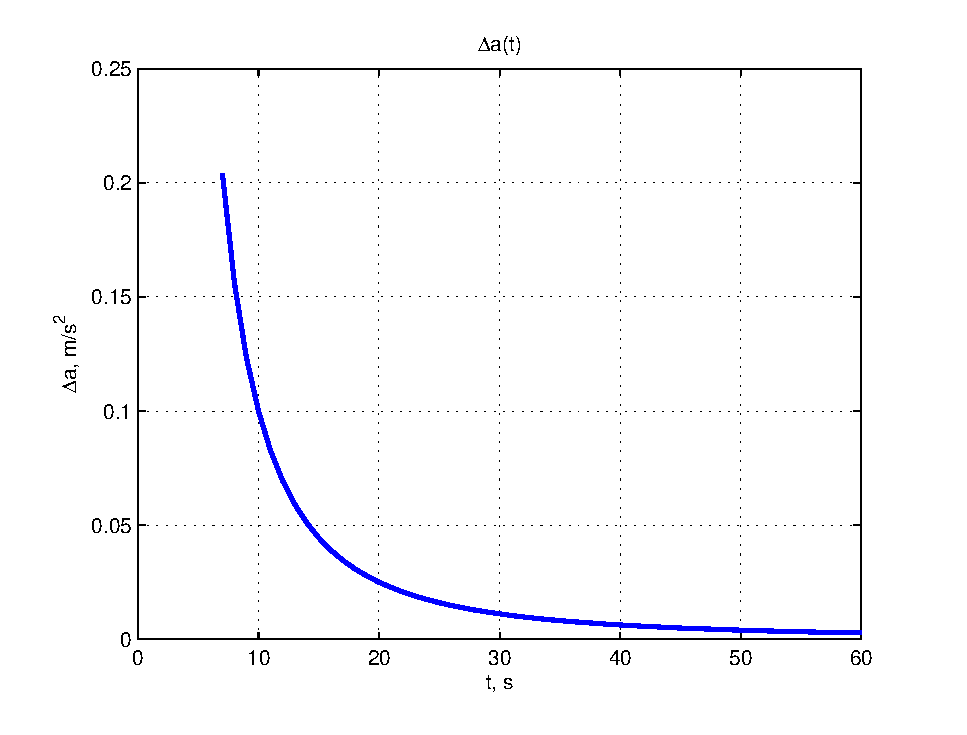
\includegraphics[scale=0.8]{acc_err}
\caption{Графік залежності значень похибок акселерометра від часу}
\label{fig:acc_err}
\end{figure} 
\vline 

\textbf{Оцінка помилки датчика кутової швидкості}

Якщо вимірник кутової швидкості об'єкта має погрішність $\Delta \vartheta '$, то приладове значення кутової швидкості

\[\dot{\vartheta }'^{*} =\dot{\vartheta }'-\Delta \dot{\vartheta }'.\] 

При цьому, будуть мати місце помилки у визначенні інших параметрів.

Підставляючи значення параметрів $\dot{\vartheta }'^{*} $ і  $\lambda _{y}^{*} $ рівняння \eqref{eq:2_51},  
після перетворень з врахуванням другого рівняння системи \eqref{eq:err} одержимо

\begin{equation} 
\label{eq:2_54_} 
\Delta \ddot{\lambda }_{y} +\frac{a_{\eta } +g_{0} }{R_{\text{З}} } \Delta \lambda _{y} =-\frac{a_{\eta } +g_{0} }{R_{\text{З}} } \Delta \vartheta ' 
\end{equation} 

Як видно ліва частина рівняння \eqref{eq:2_54_} і в цьому випадку (при $a_{\eta } =0$) представляється рівняння 
маятника Шулера, а права частина -- фактор, що викликається, обумовленими погрішностями у вимірі $\vartheta '$кута .

Якщо вважати погрішність $\Delta \dot{\vartheta }'=\Delta \dot{\vartheta }'_{0} =const$, то $\Delta \vartheta '=\Delta \dot{\vartheta }'_{0} t$, 
при цьому рішення рівняння 
\eqref{eq:2_54_} буде (якщо $a_{\eta } =0$) наступної:

\begin{equation} 
\label{eq:2_55} 
\Delta \lambda _{y} =\Delta \dot{\vartheta }'_{0} \left(\sqrt{\frac{R_{\text{З}} }{g_{0} } } \sin \sqrt{\frac{g_{0} }{R_{\text{З}} } } \cdot t-t\right)
\end{equation} 


Як видно з виразу \eqref{eq:2_55},  погрішність у визначенні координати  $\lambda _{y} $, обумовлена 
постійною  помилкою  вимірника кутової швидкості, у першому наближенні має дві складові (рис. 2.5,\textit{б)}, 
одна  з яких  росте пропорційно  часу польоту

\[\Delta \lambda _{y0} =\Delta \dot{\vartheta }'_{0} t,\] 

а інша  змінюється з періодом маятника Шулера

\[\Delta \lambda _{y} =\Delta \dot{\vartheta }'_{0} \sqrt{\frac{R_{\text{З}} }{g_{0} } } \sin \sqrt{\frac{g_{0} }{R_{\text{З}} } } \cdot t\] 


Аналогічно \eqref{eq:acc_err} можуть бути отримані орієнтовані формули для розрахунку точносних вимог 
пропонованих до вимірників кутових швидкостей.

\[\Delta \dot{\vartheta }'_{0} =\frac{\Delta \lambda _{y} }{\left(\sqrt{\frac{R_{{\text{З}}} }{g_{0} } } \sin \left(\sqrt{\frac{g_{0} }{R_{{\text{З}}} } } \cdot t\right)-t\right)} \] 

Виходячи з вимог пропонованих до точносних характеристик визначення координат (СКО $\approx$ 5м) 
отримані орієнтовані значення похибок вимірникам кутових швидкостей, у залежності від очікуваних 
перерв у роботі супутникової системи навігації. Розрахункові значення точнісних вимоги пропонованих 
до датчиків первинної інформації, зокрема вимірникам кутових швидкостей відображені на графіку рис.\ref{fig:gyro_err}.

\begin{figure}[here]
\centering
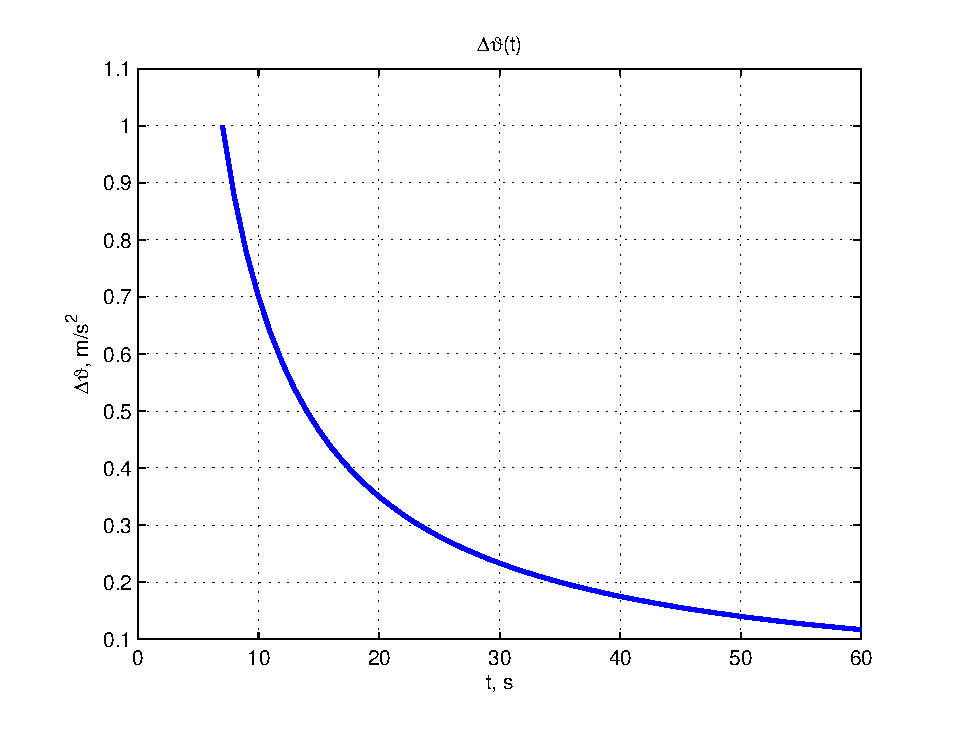
\includegraphics[scale=0.8]{gyro_err}
\caption{Графік залежності значень похибок ДКШ від часу}
\label{fig:gyro_err}
\end{figure} 



% Вихідні похибки БІНС визначаються в основному наступними складовими:
% \begin{enumerate}
%  \item похибками ДКШ і акселерометрів;
%  \item методичними похибками;
%  \item похибками обчислень 
%  \item похибками моделі використовуваної для обліку впливу гравітаційного поля на поводження інерціальних чуттєвих елементів.
% \end{enumerate}


Для БІНС розглянутого класу основний внесок у похибки визначення координат вносять датчики первинної 
інформації. Необхідно відзначити, що методичні похибки, у тому числі похибки, зв'язані зі спрощеннями 
кінематичних рівнянь БІНС, похибками моделювання форми Землі і похибками моделі гравітаційного поля, 
повинні бути не більше  похибок, внесених датчиками первинної інформації.

Багато складові вихідні похибки залежать від параметрів траєкторії й умов роботи, коефіцієнти моделі 
похибок істотно залежать від рівня вібрації і температури. Тому для більш детального дослідження 
точністних характеристик  БІНС необхідна вихідна інформація про аеродинамічні й інерційно масові 
характеристиках літака, а також параметри траєкторії. У цьому випадку можна буде провести детальні 
статистичні дослідження точністних характеристик з урахуванням впливу динамічних похибок датчиків первинної інформації.

Однак при моделюванні враховувалися тільки деякі складові:
\begin{enumerate}
  \itemсистематичні;
  \itemперекручування масштабного коефіцієнта;
  \itemвипадкові складові;
  \itemзони нечутливості
\end{enumerate}

Випадкові складові і перекручування масштабного коефіцієнта моделювалися 
з використанням генераторів "білого шуму" і формуючих фільтрів. При цьому 
вважалося, що кожен чуттєвий елемент цілком визначається значеннями цих 
складових, а самі ці складові змінюються таким чином, що при збільшенні 
одного з них зростають і всі інші. У табл. \ref{tab:gyro_err} та \ref{tab:acc_err}  
показані приклади зміни складових  похибок датчиків первинної інформації.

\begin{table}[here]
\centering
\caption{Параметри акселерометрів}

\begin{tabular}{|p{80mm}|p{20mm}|p{20mm}|p{20mm}|} \hline 
\multicolumn{4}{|p{1in}|}{Акселерометри} \\ \hline 
Зсув показань, $10^{-3}$ & 0,01 & 0,05 & 0,1 \\ \hline 
Масштабний коефіцієнт & 0,001 & 0,005 & 0,01 \\ \hline 
Неортогональність кут.с & 10 & 10 & 20 \\ \hline 
Випадкова складова, м/с3/год & 0,009 & 0,01 & 0,02 \\ \hline 

\end{tabular}
\label{tab:acc_err}
\end{table}


\begin{table}[here]
\centering
\caption{Параметри ДКШ}

\begin{tabular}{|p{80mm}|p{20mm}|p{20mm}|p{20mm}|} \hline
\multicolumn{4}{|p{1in}|}{ДКШ} \\ \hline 
Дрейф, що не залежить від перевантаження, град/год & 0,005 & 0,01 & 0,1 \\ \hline 
Дрейф, що залежить від перевантаження, град/год & 0,0075 & 0,015 & 0,15 \\ \hline 
Масштабний коефіцієнт & 0,0025 & 0,005 & 0,02 \\ \hline 
Неортогональність кут.с & 20 & 60 & 120 \\ \hline 
Випадкове блукання, град/год & 0,0005 & 0,001 & 0,01 \\ \hline 
\end{tabular}
\label{tab:gyro_err}
\end{table}

% Chapter 3
\newpage
\ESKDthisStyle{formII}
\section{Розробка автоматизованої системи діагностування}

Для розробки автоматизованої системи діагностування був використаний підхід до оптимізації параметрів за допомогою діаграм стійкості. Методика отримання таких діаграм в загальному вигляді описана в попередньому розділі. Тим не менше, дані методи не можуть бути використані для чисельного моделювання та дослідження. З цією метою для отримання діаграми стійкості САУ був розроблений чисельний ітеративний метод виділення країв. Для отримання ж конкретних кількісних і якісних характеристик САУ були використані вже існуючі алгебраїчні та частотні алгоритми дослідження.

Нижче наведені методи, що використані в ході розробки програмного забезпечення 
автоматизованої системи діагностування САУ ПС. Дані методи розбиті на підгрупи 
за своїм призначенням:

\begin{enumerate}
 \item Матричні методи
  \subitem Швидке обчислення визначників;
  \subitem Обчислення власних чисел матриці;
  \subitem Методи поліноміальної арифметики;
 \item Конверсійні методи
  \subitem Метод формування матриці Гурвіца-Раута;
  \subitem Метод перетворення передатної функції до форми Коші;
 \item Методи обробки даних
  \subitem Метод найменших квадратів;
  \subitem Методи пошуку екстремуму;
 \item Методи роботи з передатними функціями
 \subitem спрощення складних передатних функцій;
 \subitem приведення поліномів передатної функції до нормальної форми;
 \subitem метод побудови ЛАЧХ;
 \subitem метод побудови АФЧХ;
 \subitem критерій стійкості Гурвіца – Раута;
 \subitem метод побудови діаграми стійкості.
\end{enumerate}

Оскільки більшість алгоритмів, що наведені вище, носять прикладний характер, слід розглянути ті з них, які прямо впливають на ефективність роботи програмного забезпечення.

\subsection{Розробка алгоритмів алгебраїчного дослідження стійкості САК}
\subsubsection{Критерій стійкості Гурвіца-Раута}

<<Для стійкості системи n-ого порядку необхідно і достатньо, щоб n визначників, 
складених з коефіцієнтів характеристичного рівняння 

$$A(p) = a_n p^n + a_{n-1} p^{n-1} + \ldots + a_2 p^2 + a_1 p + a_0 = 0$$ 

були додатніми.>>

При цьому визначники беруться як головні мінори матриці вигляду:
\[
\begin{array}{ccccccccc}
a_{n-1} & a_{n-3} & a_{n-5} & a_{n-7} & \cdots & 0 & 0 & 0 & 0\\
a_{n} & a_{n-2} & a_{n-4} & a_{n-6} & \cdots & 0 & 0 & 0 & 0\\
0 & a_{n-1} & a_{n-3} & a_{n-5} & \cdots & 0 & 0 & 0 & 0\\
0 & a_{n} & a_{n-2} & a_{n-4} & \cdots & 0 & 0 & 0 & 0\\
\vdots & \vdots & \vdots & \vdots & \ddots & \vdots & \vdots & \vdots & \vdots\\
0 & 0 & 0 & 0 & \cdots & a_{3} & a_{1} & 0 & 0\\
0 & 0 & 0 & 0 & \cdots & a_{4} & a_{2} & a_{0} & 0\\
0 & 0 & 0 & 0 & \cdots & a_{5} & a_{3} & a_{1} & 0\\
0 & 0 & 0 & 0 & \cdots & a_{6} & a_{4} & a_{2} & a_{0}\end{array}\]


%  Chapter 4
\newpage
\ESKDthisStyle{formII}
\section{Аналіз та вибір методів оцінювання та корекції в комплексній інерціально-супутниковій системі}

Основними задачами пілотажно-навігаційних комплексів (ПНК) як постачальника 
інформаційного забезпечення польоту ЛА є сумісна обробка навігаційної інформації, 
яка надходить на борт ЛА та забезпечення високої надійності функціонування бортових 
систем та комплексів ЛА і взагалі безпеки польоту за рахунок резервування 
джерел інформації. Висока ефективність використання інформації, яка 
надходить на борт ЛА, забезпечується застосуванням різних методів її обробки. 

Найкращі результати підвищення якісних характеристик вимірювальних комплексів 
досягаються  в системах зі структурною надмірністю, коли існує можливість 
отримання пілотажно-навігаційної інформації паралельно декількома способами з 
використанням інформації від приладів та вимірювальних систем, що входять до 
складу ПНК. Отримана таким чином інформація комплексується.

В існуючих ПНК широке розповсюдження знайшли такі способи сумісної обробки 
інформації, що надходять від декількох вимірників, як взаємна компенсація і 
фільтрація похибок вимірювальних приладів, що вимірюють один і той самий 
навігаційний параметр та оптимальне оцінювання вектора стану з використанням 
апріорної інформації про контрольований процес та поточні вимірювання.

Методи оптимальної обробки інформації в ПНК використовуються з метою 
отримання оцінок вектора стану повітряного судна (або деякої частини 
цього вектора) в умовах впливу випадкових збурень і завад на процес 
вимірювання. При цьому оцінюються не самі параметри польоту, а їхні похибки. 
За оптимальної обробки пілотажно - навігаційної інформації в ПНК найважливішим 
процесом є процес отримання оптимальних оцінок. В основу алгоритмів отримання 
оптимальних оцінок можуть бути покладені такі методи обробки інформації:
\begin{itemize}
 \item метод найменших квадратів;
 \item метод максимуму правдоподібності;
 \item рекурентний неоптимальний фільтр;
 \item оптимальний фільтр Калмена.
\end{itemize}


\subsection{Рекурентний фільтр Калмана}

Термін оптимальна фільтрація відносять до методики оцінки стану динамічної системи, з якої ми 
спостерігаємо непрямі вимірювання. Стан відносить до фізичного стану, який може бути описаний 
динамічними змінними, такими як позиція, швидкість та прискорення рухомого об'єкту. Шум в вимірах 
означає, що  існує деяка  степінь невизначеності в них. Динамічна система залучає функції часу, 
а також шум в динаміці системи,  система не може бути змодельована як повністю детерміністичний 
процес. З цього боку, термін фільтрація  означає фільтрацію шуму в вимірах і забезпечення 
оптимального оцінювання змінних стану системи по відповідним вимірам і висунути припущення 
щодо динаміки системи.

Оптимальний фільтр Калмана \cite{bib:kalman_1} — ефективна і гнучка процедура для об'єднання інформації із зашумлених 
датчиків для оцінки стану стохастичної системии.
Фільтра включає 2 типа змінних:
\begin{enumerate}
 \item Вектор стану системи, включає наступні компоненти:
  \begin{itemize}
    \item Змінні, які безпосередньо нас цікавлять (необхідно знайти, наприклад швидкість, прискорення)
    \item Змінні, які безпосередньо не використовуються, але необхідні для процесу оцінювання. 
    В загальному випадку не важливо знати їхні значення, але необхідно визначити їх для для 
    покращення точності оцікни.
    \item Фільтр Калмана у специфічних задача має включати всі ті змінні динаміки системи, які можуть 
    бути виміряні ДПІ.
    \end{itemize}
 \item Коваріаційна матриця: міра невизначеності оцінювання. Рівняння, що використовуються для 
отримання коваріаційної матриці ( рівняння Рікатті) та управління невизначеністю, визначають 
як шум датчиків та динаміка невизначеності впливають на невизначеність стану системи, що оцінюється.
\end{enumerate}

За допомогою отримання невизначеності власне системи і невизначеності у відповідних 
показника датчиків, ФК дає можливість комплексувати данні з усіх ДПІ “отимально”, в 
сенсі, що результуюча оцінка мінімізує квадратичну функцію помилки оцінки, включаючи 
мінімальне середньо квадратичне відхилення будь-якої лінійної комбінації помилок оцінювання. 
Коефіцієнт підсилення Калмана — оптимальна зважена матриця, що поєднує данні ДПІ з попередньою 
оцінкою, для отримання нової апостеріорної оцінки.


\textbf{Рівняння динамічної системи}

Фільтр Калмана намагається оцінити стан змінної $x\in \Re^{n}$ дискретно управляємий
процес, що описується лінійним стохастичним диференціальним рівнянням
\begin{equation}
\label{eq:linear_sys}
x_{k} = \Phi x_{k-1} + w_{k-1},
\end{equation}
З вимірюваннями  $Z\in \Re^{m}$:
\begin{equation}
\label{eq:linear_sys_measure}
z_{k} = Hx_{k} +v_{k},
\end{equation}

Випадкові змінні $w_{k}$ та $v_{k}$ представляють шум системи (process noise) та 
шум вимірювань (measurement noise), які вважаються незалежними один від одного,
білими з нормальним розподілом шумами.
\begin{equation}\label{eq:pw} p(w)\sim N(0,Q),\end{equation}
\begin{equation}\label{eq:pv} p(v)\sim N(0,R).\end{equation}

На практиці, коваріаційна матриця шуму системи \textbf{Q} та коваріаційна
матриця шуму вимірювань \textbf{R} можуть змінюватись на кожному кроці вимірювань,
але для простоти в нашому випадку вони постійні.

Матриця $\Phi$ розміром $n \times n$ в диференціальному рівнянні \eqref{eq:linear_sys}
проводить залежність між попереднім станом системи $k-1$ та поточним станом
$k$, при наявності вхідного сигналу чи шуму. Матриця \textbf(H) $m \times n$ в 
рівнянні \eqref{eq:linear_sys_measure} відповідає вимірюванням $z_{k}$. 

\textbf{Отримання рівнянь фільтра}

Позначимо $\hat{x}(-) \in \Re^{n}$ --- апріорна оцінка на кроці $k$ 
інформація про рух системи до кроку $k$, та $\hat{x}(+) \in \Re^{n}$
апостеріорна оцінка на кроці $k$ за допомогою вимірювань $z_{k}$. 
Відповідно апріорна оцінка коваріації помилки:
\begin{equation}
\label{eq:p_minux}
P_{k}(-)= E[(x_{k}-\hat{x}_{k}(-))(x_{k}-\hat{x}_{k}(-))_{T}]
\end{equation}
та апостеріорна коваріаційна матриця помилок:
\begin{equation}
\label{eq:p_plus}
P_{k}(+)= E[(x_{k}-\hat{x}_{k}(+))(x_{k}-\hat{x}_{k}(+))_{T}]
\end{equation}

При виведенні рівнянь фільтра Калмана, наша ціль -- знайти рівняння, що 
розраховують апостеріорну оцінку стану $\hat{x}_{k}(+)$ як лінійна компенсація
апріорної оцінки стану $\hat{x}_{k}(-)$ та взваженої різниці між безпосередньо
вимірами $z_{k}$ та їх прогнозом $H\hat{x_{k}}$, як показано нижче \eqref{eq:k_update}
\begin{equation}
  \label{eq:k_update}
 \hat{x}_{k}(+)= \hat{x}_{k}(-) + K\left(z_{k}-H\hat{x}_{k}(-)\right)
\end{equation}
Різниця $(z_{k}-H\hat{x}_{k}(-))$  -- називається інноваціями (innovation) 
або залишками (residual). Залишки, як відображення дисперсії між прогнозованими
вимірами $H\hat{x}_{k}(-))$ та безпосередніми вимірами $z_{k}$. Залишок, який
рівний нулю, означає, що обоє вимірів знаходяться в повному узгодженні.

Матриця \textbf{K} $n \times m$ визначає коефіцієнт підсилення або фактор
змішування, який мінімізує апостеріорну помилку оцінки \eqref{eq:p_plus}.
Мінімізація може бути закінчена підстановкою \eqref{eq:k_update} у подане 
вище визначення для коваріації \eqref{eq:p_plus}, виконуючи необхідні дії та
взявши похідну по \textbf{K}, встановивши результат рівним нулю, а потім
вирішуючи відносно \textbf{K} рівняння. Результат може бути отриманий в 
наступній формі:
\begin{equation}
  \label{eq:k_gain}
  K_{k}=P_{k}(-)H^{T}(HP_{k}(-)H^{T}+R)^{-1} = \frac{P_{k}(-)H^{T}}{HP_{k}(-)H^{T}+R} 
\end{equation}
Зважаючи на \eqref{eq:k_gain}, якщо коваріаційна матриця помилок вимірювання
\textbf{R} прямує до нуля, коефіцієнт підсилення \textbf{K} взважує залишки 
більш сильно.Наприклад:
\begin{equation}
  \label{eq:lim_R}
  \displaystyle\lim_{R_{k}\to 0} K_{k} = H^{-1}
\end{equation}
Якщо апріорна оцінка коваріаційної матриці $P_{k}(-)$ наближається
до нуля, коефіцієнт підсилення \textbf{K} майже не взважує залишки.
\begin{equation}
  \label{eq:lim_P_minus}
  \displaystyle\lim_{P_{k}(-)\to 0} K_{k} = 0
\end{equation}

З іншого боку, взважування за допомогою \textbf{K}, у випадку коли коваріація 
помилки вимірювань \textbf{R} наближається до нуля, то безпосереднім вимірам
$z_{k}$ довіряється все більше і більш, коли прогнозовані виміри $H\hat{x}_{k}(-))$
враховуються все менше. Але якщо апріорна коваріація помилки $P_{k}(-)$ наближається
до нуля то спостерігання $z_{k}$ майже не враховуються, коли відповідно
прогнозовані виміри $H\hat{x}_{k}(-))$ стають більш ``впливовими''.


\subsection{Алгоритм фільтра Калмана}

ФК знаходить стан системи за допомогою форми зворотнього зв'язку: фільтр
оцінює стан процесу в один момент часу, а потім отримує зв'язок в формі
зашумлених вимірів. Такі рівняння для фільтра розділяються на дві групи: 
прогноз та корекція на основі вимірів. Прогноз відповідає за екстраполяцію
в часі поточного стану системи та її коваріації для отримання апріорної
оцінки для наступного кроку. Рівняння корекції необхідні для зворотнього
зв'язку -- використовують нові виміри і апріорні оцінки для отримання 
апостеріорних оцінок.

Для фільтра не важливо з якого кроку починати, так і рівняння можуть бути 
представлені з точки зору прогнозу та корекції Рис.\ref{fig:basic_cycle}
\begin{figure}[here]
\centering
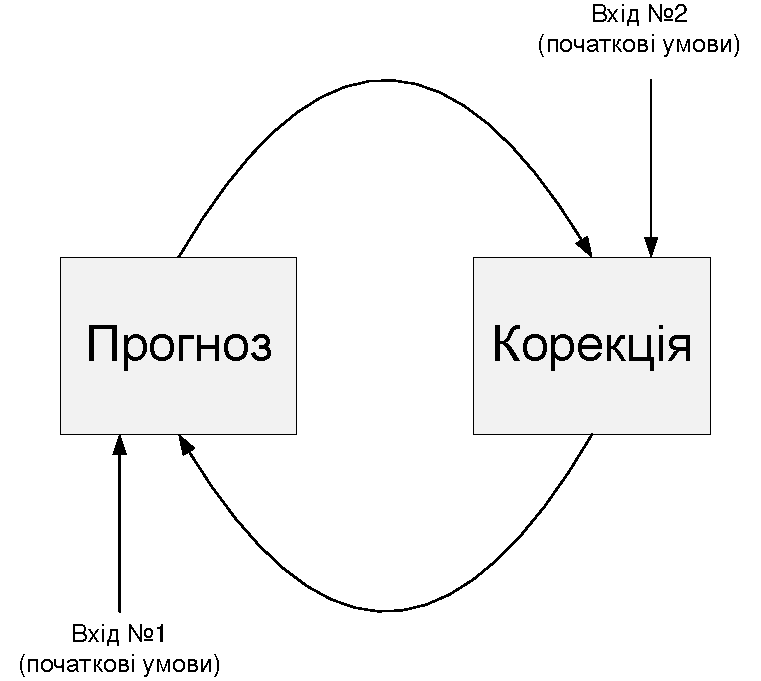
\includegraphics[scale=0.55]{pre_upd}
\caption{Цикл функціонування фільтра Калмана }
\label{fig:basic_cycle}
\end{figure} 



\begin{table}[here]
\small
\caption{Рівняння дискретного фільтра Калмана}
\centering
\begin{tabular}{|p{160mm}|} \hline 


Рівняння / Формула \\ \hline 
\begin{eqnarray} 
% \begin{array}{cc}
\text{Модель динаміки системи}  &  \label{eq:kalman_1} x_{k} = \Phi x_{k-1} + w_{k-1}, \\  
\text{Модель вимірювань}  & \label{eq:kalman_2} z_{k} = Hx_{k} +v_{k} \\ 
\text{Початкові умови}  &\label{eq:kalman_3} E[x_{o}] = \hat{x}_{0}, E[x_{o} x_{o}^{T}] = P_{0} \\
\text{Припущення незалежності}  &  \label{eq:kalman_4} E[w_{k} v_{j}^{T}] = 0 \text{для всіх k та j} \\
\text{Екстраполяція оцінки (прогноз)}  &  \label{eq:kalman_5} \hat{x}_{k}(-) = \Phi \hat{x}_{k-1}(+)\\
\text{Екстраполяція коваріації}  &  \label{eq:kalman_6} P_{k}(-) = \Phi_{k-1} P_{k-1}(+)\Phi_{k-1}^{T} + Q_{k-1} \\ 
\text{Корекція оцінки}  &  \label{eq:kalman_7} \hat{x}_{k}(+) = \hat{x}_{k}(-) + K_{k}[z_{k}-H_{k}\hat{x}_{k}(-)]\\
\text{Корекція оцінки коваріації}  &  \label{eq:kalman_8} P_{k}(+) = [I - K_{k}H_{k}]P_{k}(-)\\
\text{Коефіцієнт підсилення Калмана}   &  \label{eq:kalman_9} K_{k}= P_{k}(-)H_{k}^{T}[H_{k}P_{k}(-)H_{k}^{T} + R_{k}]^{-1}  
% \end{array}
\end{eqnarray} 
\\  \hline
\end{tabular}
\label{tb:ac}
\end{table}
Перше завдання при корекції -- розрахувати коефіцієнт підсилення Калмана, $K_{k}$/
Наступний крок, безпосередньо отримати виміри $z_{k}$, а потім генерувати 
апостеріорну оцінку за допомогою \eqref{eq:k_update}. Останній крок  -- це 
отримання апостеріорної коваріаційної матриці оцінки помилки.

Після кожного разу екстраполяції та корекції, процес повторюється, попередні
апостеріорні оцінки використовуються для прогнозу нових апріорних оцінок.
Ця рекурсивна природа є найбільш важливою особливістю фільтра Калмана, це робить
його більш практичним, в порівнянні з іншими фільтрами (наприклад фільтр Віннера)
\begin{figure}[here]
\centering
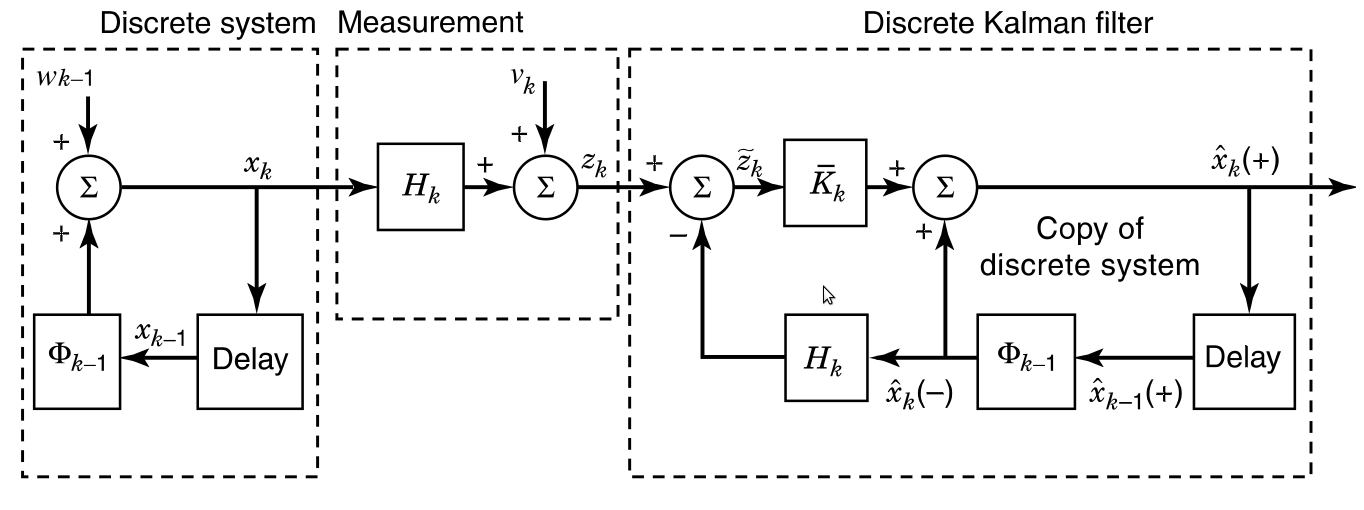
\includegraphics[scale=0.35]{kalman_flow}
\caption{Блок діаграма системи, моделі вимірювань та дискретного ФК}
\label{fig:kalman_flow}
\end{figure} 

\subsection{Проектування фільтра Калмана}

В практичній реалізації фільтра, коваріація вимірюваного шуму R вимірюється
звичайно до використання фільтра. Знаходження цієї матриці в загальному випадку
практична задача, виміряні величини дають можливість визначити дисперсію шуму, що
діє на данні датчиків.

Визначення коваріації шуму системи Q в загальному більш складна задача,
просто не має можливості безпосередньо спостерігати процес який оцінюється.
Інколи відносно проста модель процесу може дати прийнятний результат, якщо
введена достатня величина невизначеності процесу через вибір матриці Q.

В іншому випадку, є чи немає раціональної бази для вибору параметрів, часто
краща продуктивність (з точки зору статистики) може бути отримана за допомогою
налаштування параметрів фільтра Q та R. 

Асиметрія коваріаційної матриці $P$ один з факторів, що впливає на чисельну
нестійкість рівняння Рікатті. Якщо не використовується фільтр з квадратним
коренем, тоді ця матриця може бути ``симетризована'' просто за наступною 
формулою:
\begin{equation}
 \label{P_symetry}
P= \frac{1}{2}(P+P^{T})
\end{equation}
Цей метод використовується протягом довгого часу і добре себе зарекомендував.

При проектуванні фільтра, корекція коваріаційної матриці \eqref{eq:kalman_6} та
\eqref{eq:kalman_8} має бути перевірена не тільки на симетрію але й на 
додатно визначеність.
Якщо ці умови не будуть виконуються, це свідчить про помилки в програмі або
матриця погано обумовлена. Для усунення проблеми обумовленості використовується
інше рівняння для $P_{k}(+)$, яке називається формою Джозефа \cite{joseph}, яка показна на
наступному рівнянні:
\begin{equation}
 \label{P_plus_Joseph}
P_{k}(+)=[I-K_{k}H_{k}]P_{k}(-)[I-K_{k}H_{k}]^{T}+K_{k}R_{k}K_{k}^{T}
\end{equation}
З рівняння видно, що права частина є сумою двох симетричних матриць.
Перша додатно визначена інша не від'ємно визначена, що робить $P_{k}(+)$ 
додатно визначеною матрицею.

Безперечно саме фільтр Калмана найбільш привабливий при розв’язанні задачі 
комплексної обробки інформації в інерціально-супутникових системах навігації. 
Проте використання фільтра Калмана зустрічає певні труднощі при його практичної
 реалізації на борту ЛА. Зокрема в жорстко зв’язаних   інерціально-супутникових 
системах навігації,  фільтр Калмана повинний бути дуже швидкодіючим, що обмежується 
характеристиками існуючих процесорів бортових ЦОМ. 





% Chapter 5
\newpage
\ESKDthisStyle{formII}
\section{Розробка алгоримів оптимального комплексування в інерціально-супутникових
систем навігації}

Загальною вимогою для організації процесу комплексування є наявність математичних 
моделей підсистем, що підлягають комплексуванню. Сучасний стан обчислювальної техніки, 
знань в області інерціальної та супутникової навігації дозволяють скласти досить 
повні й адекватні моделі цих систем. У комплексі системи описуються на рівні їхніх 
похибок. Таким чином, для нормальної роботи комплексу потрібний адекватний опис похибок 
підсистем, включаючи неконтрольовані джерела похибок. 

\subsection{Моделі похибок  інерціальних навігаційних систем }

Рівняння похибок БІНС описують збурений режим роботи системи і є основою при аналізі 
її точності, при організації корекції, при побудові оптимальних навігаційних алгоритмів.

Матриця переходу від зв'язаної СК до географічної  СК  $B(\psi ,\vartheta ,\gamma )$ має 
вид:
\begin{equation}
\label{eq:noname_1} 
\scriptstyle
B(\psi ,\vartheta ,\gamma )=\left(
\begin{array}{ccc} 
{\scriptstyle \sin \psi \cos \vartheta } & 
{\scriptstyle\cos \psi \sin \gamma -\sin \psi \cos \gamma \sin \vartheta } & 
{\scriptstyle\cos \psi \cos \gamma +\sin \psi \sin \gamma \sin \vartheta } \\ 
{\scriptstyle\cos \psi \cos \vartheta } & 
{\scriptstyle-\sin \psi \sin \gamma -\cos \psi \cos \gamma \sin \vartheta } & 
{\scriptstyle-\sin \psi \cos \gamma +\cos \psi \sin \gamma \sin \vartheta } \\ 
{\scriptstyle\sin \vartheta } & 
{\scriptstyle\cos \gamma \cos \vartheta } & 
{\scriptstyle-\sin \gamma \cos \vartheta } 
\end{array}\right),
\end{equation}

\begin{ESKDexplanation}
\item де $\psi \left(t\right),\vartheta \left(t\right),\gamma \left(t\right)$- кути курсу, 
тангажа та крену ЛА відповідно. 
\end{ESKDexplanation}
Матриця переходу від географічної  СК до  рухомої 
екваторіальної СК $Q\left(\varphi \right)$ має вигляд:

\[Q\left(\varphi \right)=\left(\begin{array}{ccc} {1} & {0} & {0} \\ 
{0} & {\cos\varphi } & {\sin \varphi } \\ 
{0} & {-\sin \varphi } & {\cos \varphi } \end{array}\right),\] 

де $\varphi $- географічна широта.

Матриця переходу від зв'язаної СК до рухомої екваторіальної СК $C(\psi ,\vartheta,\gamma ,\varphi)$ 
задовольняє співвідношенням виду:
\[C\left(\psi ,\vartheta ,\gamma ,\varphi \right)=
Q\left(\varphi \right)\cdot B\left(\psi ,\vartheta ,\gamma \right).\] 
При розв`язанні задач повітряної навігації як основні навігаційні параметри ЛА можна 
розглядати поточні географічні координаті ( довготу $\lambda $, широту $\varphi $ и 
висоту над поверхнею земного еліпсоїда \textit{Н}), проекції шляхової швидкості $V_{E} 
,V_{N} ,V_{h} ,$а також елементи матриці переходу $B\left(\psi ,\vartheta ,\gamma 
\right)$, що характеризує орієнтацію ЛА у просторі.

Вказані навігаційні параметри задовольняє таким диференціальним рівнянням:
\begin{equation}
\left .
\begin{array}{l} 
{\dot{\lambda }=
\frac{V_{E} \left(t\right)}{\left(R_{1}+h\right)\cos \varphi \left(t\right)} } \\ 
{\dot{\varphi }=\frac{V_{N} \left(t\right)}{\left(R_{2} +h\right)} } \\
{\dot{h}=V_{h} \left(t\right)} \end{array}\right\};
\label{eq:coordinates}
\end{equation}
\begin{equation}
\dot{B}=B\Omega_{c} -\Omega_{\Gamma}B ;               
\label{eq:dBmatrix}
\end{equation}
\begin{equation}
\dot{\bar{V}}=B\bar{a}_{c} -\Delta \bar{n}\left(t\right)+\bar{g}_{T} ,     
\label{eq:dVector}
\end{equation}
\begin{ESKDexplanation}
\item де \eqref{eq:coordinates} -- рівняння для числення географічних координат; 
\item \eqref{eq:dBmatrix} -- матричне рівняння Пуассона для визначення матриці 
направляючих косинусів $B\left(\psi ,\vartheta ,\gamma \right)$; 
\item \eqref{eq:dVector} -- векторне рівняння відновно 
проекцій шляхової швидкості ЛА 
$\bar{V}=\left(\begin{array}{ccc} {V_{E} ,} & {V_{N} 
,} & {V_{h} } \end{array}\right)^{T} $; $\bar{a}_{c} \left(t\right)=\left(\begin{array}{ccc} 
{a_{x1} \left(t\right),} & {a_{y1} \left(t\right),} & {a_{z1} \left(t\right)} \end{array}
\right)^{T} $-- вектор проекцій уявного прискорення початку зв'язаної СК на її осі;
\end{ESKDexplanation}
\[\Omega_{c} =\left(\begin{array}{ccc} 
{0} & {-\omega {}_{z1} } & {\omega {}_{y1} } \\ 
{\omega {}_{z1} } & {0} & {-\omega {}_{x1} } \\ 
{-\omega {}_{y1} } & {\omega {}_{x1}} & {0} 
\end{array}\right);\] 
\[\Omega_{\Gamma } =\left(\begin{array}{ccc} 
{0} & {-(\dot{\lambda }+u)\sin \varphi } & {(\dot{\lambda }+u)\cos \varphi } \\ 
{(\dot{\lambda}+u)\sin \varphi } & {0} & {\dot{\varphi }} \\
{-(\dot{\lambda }+u)\cos \varphi } & {-\dot{\varphi }} & {0} 
\end{array}\right);\] 
\begin{ESKDexplanation}
\item $\omega_{x1}$ ,$\omega_{y1}$ ,$\omega_{z1}$-- проекції абсолютної кутової швидкості 
зв'язаної з ЛА СК на її осі; $u$-- кутова швидкість обертання Землі; 
\item $R_{1} $ и $R_{2} $-- головні радіуси кривизни обраного земного еліпсоїда;
\end{ESKDexplanation}

\[\begin{array}{l} 
{R_{1} =a\left[1-e^{2} \sin ^{2} \varphi (t)\right]^{-\frac{1}{2}};} \\ 
{R_{2} =a\left(1-e^{2} \right)\left[1-e^{2} \sin ^{2} \varphi(t)\right]^{-\frac{3}{2}};} 
\end{array}\] 
\begin{ESKDexplanation}
\item $a$,$e$-- велика піввісь и ексцентриситет земного еліпсоїда;
\item $\bar{g}_{T} =(\begin{array}{ccc}{g_{TE},}&{g_{TN},}&{g_{Th} }\end{array})^{T} $
-- вектор проекцій прискорення сили ваги на оси географічної СК;
\item $\Delta \bar{n}=\begin{array}{ccc} {\Delta n_{E} ,} & {\Delta n_{N} ,} & {
\Delta n_{h} ,} \end{array})^{T} $-- вектор проекцій суми переносного и кориолісова 
прискорень на осі географічної СК;
\end{ESKDexplanation}
\[\begin{array}{l} 
{\Delta n_{E} =\frac{V_{E} V_{h} }{R_{1} +h} -\frac{V_{E} V_{N}}{R_{1} +h} tg\varphi +2u\left(V_{h} \cos \varphi -V_{N} \sin \varphi \right);} \\ 
{\Delta n_{N} =\frac{V_{N} V_{h} }{R_{2} +h} +\frac{V_{E}^{2} }{R_{1} +h} tg\varphi+2uV_{E} \sin \varphi ;} \\ 
{\Delta n_{h} =-\frac{V_{E}^{2} }{R_{1} +h} -\frac{V_{N}^{2}}{R_{2} +h} -2uV_{E} \cos \varphi ;} 
\end{array}\] 
\begin{ESKDexplanation}
\item $\bar{g}_{T} =\left[0,0,g_{e} \right]^{T} $-- вектор проекцій нормального 
прискорення сили ваги на осі географічної СК 
$g_{e}=\mu//a^{2}$, $\mu=398600,44\cdot 10^{9} \left[\text{м}^{3}/c^{2} \right]$
\end{ESKDexplanation}


Маючи інформацію  про вихідні координати та проекції шляхової швидкості ЛА, про вихідну 
матрицю орієнтації $B_{0}$ (її визначення є предметом задачі початкового виставлення  
БІНС ), а також про моделі прискорення сили ваги $g^{T}$($\varphi $, $\lambda $, \textit{h}), 
на основі рівнянь \eqref{eq:coordinates}$\div $\eqref{eq:dVector} с використанням  
поточних показів ДУС и акселерометрів можна отримати поточні значення  шуканих навігаційних 
параметрів ЛА.

При точному завдані вихідних умов и при точній  моделі прискорення сили ваги, а також 
при відсутності похибок інерціальних ДПІ и похибок обчислення в наслідок інтегрування 
рівнянь \eqref{eq:coordinates}$\div $\eqref{eq:dVector}  будуть отримані істинні 
значення основних навігаційних параметрів ЛА.

Похибки завдання вихідних координат и проекцій шляхової швидкості ЛА, похибки  початкового 
виставлення , аномальні варіації прискорення сили ваги, похибки інерціальних ДПІ, 
методичні похибки алгоритмів обчислення и похибки через  кінцеву довжину розрядній 
сітці обчислювача (похибки округлення) будуть приводити до похибок визначення шуканих 
навігаційних параметрів ЛА.

У лінійному наближенні еволюція похибок БІНС у визначенні основних навігаційних параметрів 
у часі може бути описана лінійними диференціальними рівняннями похибок.

Рівняння похибок БІНС у визначенні координат випливає з динамічних рівнянь числення 
координат, що наведені в алгоритмах БІНС і мають вигляд:

\begin{equation} 
\label{eq:dRsdins} 
\begin{array}{l} 
{\Delta \dot{R}_{E} =\Delta V_{E}(t)\cdot \frac{R_{\text{З}} }{R\cos \varphi (t)} 
+\Delta R_{N} (t)\frac{V_{E}^{}(t)\sin \varphi (t)}{R_{\text{З}} R\cos ^{2} \varphi (t)} 
-\Delta h(t)\frac{R_{\text{З}} V_{E}^{}(t)}{R^{2} \cos \varphi (t)} ;} \\ 
{\Delta \dot{R}_{N} =\Delta V_{N}(t)\cdot \frac{R_{\text{З}}}{R} -\Delta h(t)\frac{R_{\text{З}} V_{N}(t)}{R^{2}};} \\ 
{\Delta \dot{h} =\Delta V_{h} (t);} \end{array} \end{equation} 
\begin{ESKDexplanation}
\item де $\Delta R_{E} (t)=\Delta \lambda (t)R_{\text{З}}$, $\Delta R_{N}(t)=\Delta\varphi(t)R_{\text{З}} $
-- похибка БІНС у визначенні приведених координат місцезнаходженняЛА; 
\item $\Delta \lambda(t)$,$\Delta \varphi (t)$,$\Delta H(t)$-- похибки БІНС у визначенні 
географічних координат; $\Delta V_{E}(t),\Delta V_{N}(t),\Delta V_{H}(t)$-- похибки 
БІНС у визначенні проекції шляхової швидкості ЛА; 
\item $R=R_{\text{З}}+H$; $R_{\text{З}}$  -- радіус земної сфери; 
\end{ESKDexplanation}
Еволюція похибок БІНС у визначенні проекції шляхової швидкості ЛА $\Delta V_{E}^(t)$,
$\Delta V_{N}(t)$,$\Delta V_{h}(t)$, також може бути отримана з динамічних 
рівнянь числення шляхової швидкості в алгоритмах БІНС, і описується наступною системою 
рівнянь: 
\begin{equation}
\begin{array}{l}{\Delta \dot{V}_{E} =a_{N} \alpha_{h} -a_{h} \alpha_{N} +\sum_{i=1}^{3}b_{1,i}  \Delta a_{i} -\Delta V_{h} U(t)\cos \varphi +\Delta V_{N}U(t)\sin \varphi +} \\ 
{+\frac{\Delta R_{N} }{R_{\text{З}} } \left(U(t)(V_{h} \sin \varphi +V_{N}\cos \varphi \right))-(\frac{\Delta V_{E} }{R\cos \varphi } +\frac{V_{E} \sin \varphi}{R\cos ^{2} \varphi } \frac{\Delta R_{N} }{R_{\text{З}} } )\times } \\ 
{\times (V_{h} \cos \varphi -V_{N} \sin \varphi )+\frac{\Delta hV_{E} }{R^{2} } (V_{h} -V_{N}tg\varphi);} \\
\\
{\Delta \dot{V}_{N} =-a_{E}\alpha_{h} +a_{h} \alpha_{E} +\sum_{i=1}^{3}b_{2,i}  \Delta a_{i} -\Delta V_{E}U(t)\sin \varphi -\Delta V_{h} \dot{\varphi }(t)-} \\ 
{-\frac{\Delta R_{N} }{R_{\text{З}}} V_{E} U(t)\cos \varphi -\frac{\Delta V_{N} }{R} V_{h} -(\frac{\Delta V_{E} }{R\cos \varphi } +\frac{V_{E} \sin \varphi }{R\cos ^{2} \varphi } \frac{\Delta R_{N} }{R_{\text{З}} } )V_{E} \sin \varphi +} \\ 
{+\frac{\Delta h}{R^{2} } (V_{E}^{2} tg\varphi +V_{N} V_{h} );} \\
\\
{\Delta \dot{V}_{h} =a_{E} \alpha_{N} -a_{N} \alpha_{E} +\sum_{i=1}^{3}b_{3,i}  \Delta a_{i} +\Delta V_{E} U(t)\cos \varphi +\Delta V_{N} \dot{\varphi }(t)-} \\ 
{-\frac{\Delta R_{N} }{R_{\text{З}} } V_{E} U(t)\sin \varphi +\frac{\Delta V_{N} }{R} V_{N} +(\frac{\Delta V_{E} }{R\cos \varphi } +\frac{V_{E} \sin \varphi }{R\cos ^{2} \varphi } \frac{\Delta R_{N} }{R_{\text{З}} } )V_{E} \cos \varphi +} \\ 
{+g_{e} \left(-\frac{2\Delta h}{a} +\frac{3}{2} e^{2} \sin \varphi \cos \varphi \frac{\Delta R_{N} }{R_{\text{З}} } \right)-\frac{\Delta h}{R^{2} } \left(V_{E}^{2} +V_{N}^{2} \right),} 
\end{array}
\label{eq:dVsdins}
\end{equation}
\begin{ESKDexplanation}
\item де $b_{ij}$ (i,j=1,2,3) -- елементи матриці направляючих косинусів \textbf{B}; 
\item $\Delta a_{i}$ (i=1,2,3) -- приведені похибки акселерометрів БІНС (з урахуванням 
похибок чисельного інтегрування рівняння  у бортовому обчислювачі); 
\item $a_{H}$ ,$a_{E}$,$a_{N}$ -- поточні значення проекцій уявного прискорення початку зв'язаної СК на 
осі географічної СК; 
\item $\alpha_{H}$, $\alpha_{E}$, $\alpha_{N}$ -- похибки моделювання 
в БІНС орієнтації географічного координатного тригранника ($\alpha_{E} $;
\item $\alpha_{N} $-- похибки побудови вертикалі, $\alpha_{H} $-- азимутальна похибка); 
\item $R=R_{\text{З}} +H$ -- поточна висота; 
\item $U(t)=2\Omega_{\text{З}} +\dot{\lambda }(t)$; $dot{\varphi}(t)=\frac{V_{N}}{R}$; $\dot{\lambda }(t)=\frac{V_{E}}{R\cos \varphi }.$ 
\end{ESKDexplanation}
  Аналіз показує, що еволюція параметрів $\alpha_{h}$, $\alpha_{E}$, $\alpha_{N}$ у часі описується наступною системою рівняннь:
\begin{equation} 
\label{eq:dasdins} \begin{array}{l} 
{\dot{\alpha }_{E} =-\omega_{N} \alpha_{h} +\omega_{h} \alpha_{N} -\frac{\Delta V_{N} }{R} -\sum_{i=1}^{3}b_{1,i}\varepsilon_{i} ,} \\
{\dot{\alpha }_{N} =-\omega_{h} \alpha_{E} +\omega_{E} \alpha_{h} +\frac{\Delta V_{E} }{R} -u\sin \varphi \frac{\Delta R_{N} }{R_{7} }
-\sum_{i=1}^{3}b_{2,i}  \varepsilon_{i} ,} \\ 
{\dot{\alpha }_{h} =-\omega_{E} \alpha_{N} +\omega_{N} \alpha_{E} +\frac{\Delta V_{E} }{R} tg\varphi +(u\cos \varphi +\frac{V_{E} }{R\cos ^{2} \varphi } )
\frac{\Delta R_{N} }{R_{7} } -\sum_{i=1}^{3}b_{3,i}\varepsilon_{i} ,} \end{array} \end{equation} 

\begin{ESKDexplanation}
\item де  $\omega_{E} =-\dot{\varphi }(t),\omega_{N} =\left[u+\dot{\lambda }(t)\right]
\cos \varphi ,\omega_{h} =\left[u+\dot{\lambda }(t)\right]\sin \varphi ,$
\item $\dot{\lambda }=\frac{V_{E} }{R\cos \varphi } ;$ $\dot{\varphi }=\frac{V_{N} }{R} $; $\varepsilon_{i}$
 (i=1,2,3)-- приведені похибкм ДУС БІНС;
\end{ESKDexplanation}
Аналіз показує, що похибки моделювання географічного тригранника $\alpha_{h} $,$\alpha_{E} $ ,
$\alpha_{N} $ зв'язані з похибками визначення координат $\Delta R_{N} $,$\Delta 
R_{E} $ і похибками моделювання орієнтації рухливої екваторіальної СК $\delta_{\xi} $, 
$\delta_{\eta } $, $\delta_{\zeta } $ такими   співвідношеннями:
\[\begin{array}{l} 
{\alpha_{E} =\delta_{\xi } -\frac{\Delta R_{N} }{R_{\text{З} } } ;} \\ 
{\alpha_{N} =\delta_{\eta } \cos \varphi -\delta \sin \varphi +\frac{\Delta R_{E} }{R_{\text{З} } } \cos \varphi ;} \\ 
{\alpha_{h} =\delta_{\eta } \sin \varphi-\delta_{\zeta } \cos \varphi +\frac{\Delta R_{E} }{R_{\text{З} } } \sin \varphi .} 
\end{array}\] 
Еволюція в часі похибок моделювання рухливої екваторіальної СК $\delta_{\xi } $, $\delta_{\eta } $,
$\delta_{\zeta } $ описується більш простими, ніж \eqref{eq:dasdins}, рівняннями:
\[\begin{array}{l} 
{\dot{\delta }_{\xi } =-(u+\dot{\lambda })\delta_{\zeta } -\varepsilon_{\zeta }(t)} \\ 
{\dot{\delta }_{\eta } =-\varepsilon_{\eta } (t)} \\ 
{\dot{\delta }_{\zeta } =-(u+\dot{\lambda })\delta_{\xi } -\varepsilon_{\zeta }(t)}\end{array};\] 
\begin{ESKDexplanation}
\item де $\dot{\lambda }=\frac{V_{E}(t)}{R\cos(t)} $.
\end{ESKDexplanation}
Якщо ввести в розгляд  інерціальну прямокутну геоцентричну СК $\xi_{u} \eta_{u} \zeta_{u} $, 
вісь $\eta_{u} $ якої збігається з віссю $\zeta $, 
а вісь $\xi_{u} $ у момент  \textit{t }= 0 лежить у площині Гринвіцького меридіана, 
то можна сказати, що похибки моделювання орієнтації такої СК $\delta_{\xi_{u}} $,
$\delta_{\eta_{u} } $,$\delta_{\zeta_{u} } $ зв'язані з параметрами $\delta_{\xi }$,
$\delta_{\eta } $,$\delta_{\zeta }$ співвідношеннями виду:
\[\begin{array}{l} 
{\delta_{\xi } =\delta_{\xi_{u} } Aos\lambda_{*} -\delta_{\xi_{u} } \sin \lambda_{*} } \\ 
{\delta_{\eta } =\delta_{\eta_{u} }} \\ 
{\delta_{\zeta } =\delta_{\xi_{u} } \sin \lambda_{*} -\delta_{\zeta_{u} } Aos\lambda_{*} } \end{array};\] 
\begin{ESKDexplanation}
\itemде  $\lambda_{*} =ut+\lambda (t)$ .
\end{ESKDexplanation}
Рівняння, що описують еволюцію в часі похибок моделювання інерціальної СК $\delta_{\xi_{u} } $,
$\delta_{\eta_{u} } $,$\delta_{\zeta_{u} } $ виявляється досить простими:

\[\begin{array}{l}{\dot{\delta }_{\xi_{u} } =-\varepsilon_{\xi_{u}} (t);} \\ 
{\dot{\delta}_{\eta_{u} } =-\varepsilon_{\eta_{u} } (t);} \\ 
{\dot{\delta}_{\zeta_{u} } =-\varepsilon_{\zeta_{u} } (t),} \end{array}\] 

де $\left(
\begin{array}{l} {\varepsilon_{\xi_{u} } } \\ 
{\varepsilon_{\eta_{{\rm u}} } } \\ 
{\varepsilon_{\zeta_{u} } } \end{array}\right)=\Delta {\bf C}(t){
\bf C}(t)\left(\begin{array}{l} {\varepsilon_{1} } \\ 
{\varepsilon_{2} } \\ 
{\varepsilon_{3} } \end{array}\right)$;

$\Delta {\bf C}(t)=\left(\begin{array}{ccccc} 
{\cos \lambda_{*} } & {} & {-\sin \lambda_{*} } & {} & {0} \\ 
{\sin \lambda_{*} } & {} & {\cos \lambda_{*} } & {} & {0} \\ 
{0} & {} & {0} & {} & {1} \end{array}\right)$ -- матриця переходу від рухливої  
екваторіальної СК до  інерціальної СК.

Таким чином, у моделі похибок БІНС можливе використання принаймні трьох груп параметрів, 
що характеризують похибки моделювання орієнтації СК:

\{$\alpha_{E} $,$\alpha_{N} $,$\alpha_{h} $\},\{$\delta_{\xi } $,$\delta_{\eta} $,
$\delta_{\zeta } $\}, \{$\delta_{\xi_{u} } $,$\delta_{\eta_{u}} $,$\delta_{\zeta_{u} } $\}.

Надалі в роботі використовуються параметри $\alpha_{E} $,$\alpha_{N} $,$\alpha_{h} $, 
що характеризують похибки  моделювання географічної СК і мають найбільш наочну 
фізичну інтерпретацію. Цим параметрам відповідають рівняння еволюції \eqref{eq:dasdins}.

Для замикання системи рівнянь похибок БІНС \eqref{eq:dRsdins}, \eqref{eq:dVsdins}, 
\eqref{eq:dasdins} необхідно вказати моделі еволюції приведених похибок ДПІ. 

З урахуванням вигляду моделі еволюції похибок ДПІ , 
рівняння похибок БІНС \eqref{eq:dRsdins}, \eqref{eq:dVsdins}, \eqref{eq:dasdins} 
можуть бути замкненні  наступними  рівняннями відносно 
$C_{\omega } $, $C_{a} $, $C_{\varepsilon} $, $D_{a} $, $\bar{\varepsilon }_{A} $, $\Delta \bar{a}_{c} $:

\begin{equation} \label{eq:dawsdins} \begin{array}{l} 
{\dot{C}_{\omega } =\xi_{A\omega } (t);} \\ 
{\dot{C}_{a} =\xi_{Aa} (t);} \\ 
{\dot{C}_{\varepsilon } =\xi_{A\varepsilon } (t);} \\ 
{\dot{D}_{a} =\xi_{Da}(t);} \\ 
{\dot{\bar{\varepsilon }}_{c} =\bar{\xi}_{A} (t);} \\ 
{\Delta \dot{\bar{a}}_{c} =\bar{\xi }_{\Delta a}(t),} \end{array} \end{equation} 
\begin{ESKDexplanation}
\item де $\xi_{A\omega } (t);$$\xi_{Aa} (t);$\item $\xi_{A\varepsilon } (t);$$\xi_{Da} (t);$
$\bar{\xi }_{A} (t);$$\bar{\xi }_{\Delta a} (t)$-- білошумні збурення відповідної розмірності, 
які характеризують дрейф квазістаціонарних  параметрів моделі ДПІ. % \eqref{eq:__6_13_}.
\end{ESKDexplanation}
Повертаючись до моделей похибок БІНС відзначимо, що коли  вектор-стовпець похибок БІНС $\bar{X}(t)$ прийняти 
у вигляді:
\[\bar{X}=(\Delta R_{E} ,\Delta R_{N} ,\Delta h,\Delta V_{E} ,\Delta V_{N} ,\Delta 
V_{h} ,\alpha_{E} ,\alpha_{N} ,\alpha_{h} ,\varepsilon_{c1} ,\varepsilon_{c2} 
,\varepsilon_{c3} ,\Delta a_{c1} ,\Delta a_{c2} ,\Delta a_{c3} ,)^{T} ,\] 
то модель еволюції похибок БІНС може бути подана у компактній формі
\begin{equation} 
\label{eq:matrix_sdins} \dot{\bar{X}}=F\bar{X}\left(t\right)+G\bar{\xi }(t), 
\end{equation} 
де F та G   --  матриці 15 $\times$ 15 і 15 $\times$ 21 відповідно; $\bar{\xi }(t)$ -- вектор-стовпець 
розмірності 21, компонентами якого є незалежні Гауссівські «білі» шуми з нульовими 
середніми значеннями и одиничними дисперсіями.

Відмінні від нуля елементи матриці $F$ мають вигляд:
\begin{equation}
\label{eq:Fsdins_} 
\begin{array}{l}
{f_{1,2} =\frac{\dot{\lambda }}{R_{\text{З}} } tg\varphi;f_{1,3} =\frac{-\dot{\lambda }R_{\text{З}} }{R};f_{1,4} =\frac{R_{\text{З}} }{R\cos \varphi } ;}\\
{f_{2,3} =\frac{-\dot{\varphi }R_{\text{З}} }{R};f_{2,5} =\frac{R_{\text{З}} }{R};f_{3,6} =1;}\\
{f_{4,2} =\frac{2u+\dot{\lambda }}{R_{\text{З}} } \left(V_{h} \sin \varphi +V_{N} \cos \varphi \right)-\frac{\dot{\lambda }}{R_{\text{З}} } tg\varphi \left(V_{h} \cos \varphi -V_{N} \sin \varphi \right);}\\
{f_{4,3}=\frac{V_{E} }{R^{2} } \left(V_{h} -V_{N} tg\varphi \right);}\\
{f_{4,4}=\frac{V_{N}\sin \varphi -V_{h} \cos \varphi }{R\cos \varphi } ;}\\
{f_{4,5}=\left(2u+\dot{\lambda }\right)\sin \varphi; f_{4,6}=-\left(2u+\dot{\lambda }\right)\cos \varphi ;}\\
{f_{4,8}=-a_{h};f_{4,9}=a_{N};f_{4,13}=b_{1,1};f_{4,14}=b_{1,2};f_{4,15}=b_{1,3};}\\
{f_{5,2}=-\frac{2u+\dot{\lambda }}{R_{\text{З}} }V_{E} \cos \varphi -\frac{V_{E}^{2} }{RR_{\text{З}} } tg^{2} \varphi ;}\\
{f_{5,3}=\frac{V_{E}^{2} tg\varphi +V_{h} V_{N} }{R^{2} } ;}\\ 
{f_{5,4}=-\left(2u+\dot{\lambda }\right)\sin \varphi;f_{5,5}=-\frac{V_{h} }{R};}\\
{f_{5,6}=-\dot{\varphi }(t);f_{5,7}=a_{h}; f_{5,9} =-a_{E};f_{5,13}=b_{2,1};f_{5,14}=b_{2,2};f_{5,15}=b_{2,3} ;}\\
{f_{6,2} =-2u\frac{V_{E}^{} \sin \varphi }{R} +\frac{3g_{e} }{2R_{\text{З}}} e^{2} \sin \varphi \cos \varphi ;}\\
{f_{6,3} =-\frac{2g_{e} }{a} -\frac{V_{E}^{2} +V_{N}^{2}}{R^{2} };f_{6,4} =\left(2u+\dot{\lambda }\right)\cos \varphi ;}\\
{f_{6,5}=\dot{\varphi }(t)+\frac{V_{N} }{R};f_{6,7} =-a_{N} ;f_{6,8} =a_{E} ;f_{6,13}=b_{3,1};f_{6,14}=b_{3,2}; f_{6,15}=b_{3,3} ;}\\ 
{f_{7,5}=-\frac{1}{R} ;f_{7,8}=\omega_{h}; f_{7,9}=-\omega_{N} ;}\\
{f_{7,10}=-b_{1,1};f_{7,11}=-b_{1,2};f_{7,12}=-b_{1,3} ;}\\ 
{f_{8,2} =-\frac{u}{R} \sin \varphi; f_{8,4} =\frac{1}{R};f_{8,7} =-\omega_{h};f_{8,9} =\omega_{E};}\\
{f_{8,10} =-b_{2,1}; f_{8,11} =-b_{2,2}; f_{8,12} =-b_{2,3} ;}\\ 
{f_{9,2} =\frac{1}{R}_{7} (u\cos \varphi +\frac{\dot{\lambda }}{\cos \varphi });}\\
{f_{9,4} =\frac{tg\varphi }{R}; f_{9,7} =\omega_{N}; f_{9,8} =-\omega_{E};}\\ 
{f_{9,10} =-b_{3,1};f_{9,11} =-b_{3,2};f_{9,12} =-b_{3,3}.}
\end{array}
\end{equation} 
Відрізні від нуля елементи матриці \textit{G}(15$\times $21) задовольняють таким 
співвідношенням:
\begin{equation} 
\label{eq:Gmatrix_} 
\begin{array}{cc} 
g_{i,i} =\sigma_{i},& i=1,..,15; \\ 
g_{i+3,j+18}=b_{i,j} \sigma_{a},& i=1,2,3,j=1,2,3;\\ 
g_{i+6,j+15}=-\sigma_{\omega } b_{i,j} & i=1,2,3,j=1,2,3; 
\end{array} 
\end{equation} 
\begin{ESKDexplanation}
\item де $\sigma_{1} \div \sigma_{15} $- середньоквадратичні значення (СКЗ) білошумних збурень, 
що характеризують вплив різних факторів ($\sigma_{1} \div \sigma_{3} $-- похибок 
численного інтегрування рівняння \eqref{eq:coordinates}; 
\item  $\sigma_{4} \div \sigma_{6} $ --  підсумковий ефект аномалій гравітаційного поля и похибок численного інтегрування 
рівняння \eqref{eq:dVector}, 
\item $\sigma_{7} \div \sigma_{9} $-- похибок численного інтегрування рівняння для параметрів орієнтації \eqref{eq:dBmatrix};  
\item $\sigma_{10} \div \sigma_{15} $ -- випадкового дрейфу квазістаціонарних зведених погрішностей 
ДПІ  $\bar{\varepsilon }_{A} $ и $\Delta \bar{0}_{A} $);
\item $\sigma_{a} $, $\sigma_{\omega } $ -- СКЗ білошумних складових погрішностей акселерометрів і ДКШ БІНС.
\end{ESKDexplanation}

Елементи матриць \textbf{F} и \textbf{G}, що випливає з аналізу співвідношень \eqref{eq:Fsdins_} 
и \eqref{eq:Gmatrix_}, залежать від поточних значень навігаційних параметрів польоту 
ЛА.

Безперервної моделі еволюції похибок БІНС  \eqref{eq:matrix_sdins} відповідає такий 
дискретний аналог:

\[\bar{X}_{k+1} =\Phi_{k} \bar{X}_{k} +G_{k} \bar{\xi}_{k} ,\] 
\begin{ESKDexplanation}
\item де $\Phi_{k}=E+F(t_{k})\Delta t$, $G_{k} =G(t_{k})\cdot \Delta t;$ 
\item $\Delta t$--  крок дискретизації часу;
\item $E$ -- одинична матриця  $15\times 15$.
\end{ESKDexplanation}

\subsection{Математичні моделі похибок супутникової системи навігації}

Для опису  похибок СНС у визначенні координат і проекцій шляхової швидкості ЛА пропонується 
використовувати математичні моделі, що містять  Марківські і гаусовські складові 
похибок:
\begin{equation} \label{eq:sns_errors} 
\begin{array}{l} 
{\Delta R_{Es,k} =\Delta R_{Ec,k} +\frac{\sigma_{Rs} }{\cos \varphi_{k} } \eta_{REs,k} +\frac{\sigma_{\delta Rs} }{\cos \varphi_{k} } \eta_{\delta RE,k} ;} \\ 
{\Delta R_{Ns,k} =\Delta R_{Nc,k} +\sigma_{Rs} \eta_{RNs,k} +\sigma_{\delta Rs} \eta_{\delta RN,k} ;} \\ 
{\Delta H_{s,k} =\Delta H_{c,k} +\sigma_{Hs} \eta_{Hs,k} +\sigma_{\delta Rs} \eta_{\delta H,k} }\\ 
{\Delta V_{ls,k} =\Delta V_{lc,k} +\sigma_{Vs} \eta_{V\, ls,k} +\sigma_{\delta Vs} \eta_{\delta V\, ls,k}, \text{при } l=E,N,H;} 
\end{array} \end{equation} 

\begin{ESKDexplanation}
\item де $\Delta R_{ls,k}$, (l=E,N); $\Delta H_{s,k}$; $\Delta V_{ls,k}$ 
 (l=E,N,H) -- похибки СНС у визначенні приведених  координат, висоти і складових 
шляхової швидкості ЛА;
\item $\Delta R_{lc,k}$ (l=E,N);  $\Delta H_{c,k}$; $\Delta V_{lc,k}$ 
 (l=E,N,H) -- корельовані (Марківські) складові  похибок СНС;
\item $\sigma_{Rs} $, $\sigma_{Hs}$ , $\sigma_{Vs}$  --  СКЗ білошумових складових 
похибок СНС;
\item $\sigma_{\delta Rs} $, $\sigma_{\delta Hs} $, $\sigma_{\delta Vs} $ -- СКЗ додаткових 
білошумових складових похибок СНС, що виникають тільки за умови, що $t_{k}$ -- момент 
зміни сузір'я навігаційних супутників; 
\item $\eta_{Rls,k}$, $\eta_{\delta Rls,k}$, (l=E,N); $\eta_{Hs,k}$ 
, $\eta_{\delta Hs,k}$; $\eta_{V\, ls,k}$ ,$\eta_{\delta V\, ls,k}$ 
 (l=E,N,H)-- стандартні білі дискретні шуми зі СКЗ.
\end{ESKDexplanation}

Корельовані складові похибок СНС описуються наступними співвідношеннями:
\begin{equation}\label{eq:sns_errors_cor} 
\begin{array}{l} 
{\Delta R_{Ec,k}=W_{R} \Delta R_{Ec,k-1} +q_{R} \frac{\sigma_{Rc} }{\cos \varphi_{k} } \eta_{REc,k} +\frac{\sigma_{\delta RC} }{\cos \varphi_{k} } \eta_{\delta REc,k} ;} \\ 
{\Delta R_{Nc,k}=W_{R} \Delta R_{Nc,k-1} +q_{R} \sigma_{Rc} \eta_{RNc,k} +\sigma_{\delta RC} \eta_{\delta RNc,k} ;} \\ 
{\Delta H_{c,k}=W_{R}  \Delta H_{c,k-1}  +q_{R} \sigma_{Hc} \eta_{Hc,k} +\sigma_{\delta Hc} \eta_{\delta Hc,k} ;} \\ 
{\Delta V_{lc,k} =W_{V} \Delta V_{lc,k-1} +q_{V}\sigma_{Vc} \eta_{V lc,k} +\sigma_{\delta Vc} \eta_{\delta V lc,k}, \text{при } l=E,N,H,} 
\end{array} \end{equation} 
\begin{ESKDexplanation}
\item де  
\[
\begin{array}{l}
{W_{R} =e^{-(\lambda_{s} V_{\text{Ш}} +\lambda_{st} )\Delta t} ; }
{q_{R} =\left[1-\exp \left(-2\left(\lambda_{s} V_{\text{Ш}} +\lambda_{st} \right)\Delta t\right)\right]^{0,5};}\\
{W_{V} =e^{-\lambda_{V} \Delta t};}
{q_{V} =\left[1-\exp \left(-2 \lambda_{V} \Delta t\right)\right]^{0,5};}
\end{array}\] 
\item $\lambda_{s} $-- показник просторової кореляції похибки СНС за координатами; 
\item $\lambda_{V} ,\lambda_{st} $-- показник часової кореляції похибок СНС за швидкістю та за 
координатами; 
\item $V_{\text{Ш}}$-- шляхова швидкість ЛА;
\item $\Delta t$-- дискрета оновлення вихідної інформації СНС у часі;
\item $\sigma_{Rc} ,\sigma_{Hc} ,\sigma_{Vc} $ -- СКЗ корельованих складових похибок СНС;
\item $\sigma_{\delta Rc} $,  $\sigma_{\delta Hc} $, $\sigma_{\delta_{Vc}} $  -- СКЗ 
додаткових гаусовських збурень у моменти зміни сузір'я навігаційних супутників;
$\eta_{Rlc,k}$ ,  $\eta_{\delta Rlc,k}$  (l=E,N),  $\eta_{Hc,k}$ 
, $\eta_{\delta Hc,k}$, $\eta_{V\, lc,k}$ ,$\eta_{\delta V\, lc,k}$ (l=E,N,H) -- 
стандартні центровані дискретні білі шуми з одиничною інтенсивністю.
\end{ESKDexplanation}

Для стандартного режиму СНС типу GPS NAVSTAR можуть бути рекомендовані наступні значення 
параметрів моделей \eqref{eq:sns_errors}, \eqref{eq:sns_errors_cor}:

\[\begin{array}{l}
{\lambda_{s} =4\cdot 10^{-6} \text{м}^{-1} ;} 
{\lambda_{st} =5\cdot 10^{-4} \text{с}^{-1}; }
{\lambda_{V} =\left(0,0017\div 0,05\right)\, \text{с}^{-1};}\\
{\sigma_{Rs} =\left(1\div 3\right) \text{м};}
{\sigma_{Hs} =\left(1,5\div 4\right)\, \text{м};}
{\sigma_{Vs} =\left(0,01\div 0,05\right) \text{м}/c;}\\
{\sigma_{\delta Rs} =\left(1\div 4\right) \text{м}; }
{\sigma_{\delta_{Vs} } =\left(0,02\div 0,2\right) \text{м}/c;} 
{\sigma_{Rc} =\left(5\div 7\right) \text{м};}\\
{\sigma_{Hc} =\left(7\div 10\right) \text{м};  }
{\sigma_{Vc} =\left(0,02\div 0,3\right) \text{м}/c;}
{\sigma_{\delta Rc} =\left(2\div 5\right) \text{м};}\\
{\sigma_{\delta_{Vc} } =\left(0,01\div 0,02\right) \text{м}/c;}
{\sigma_{\delta Hc} =\left(3\div 7\right) \text{м}.}
\end{array}\] 

% Головною задачею СНС є визначення псевдодальностей $D_{sl}^{} $ і псевдошвидкостей $V_{sl}^{} $ (l 
% = 1, \dots , N  -- число видимих навігаційних супутників),  які задовольняють співвідношенням 
% виду: 
% 
% \[\begin{array}{l} {D_{sl,k} =\{ \left[x_{l} \left(t_{k} -\tau_{l} \right)-x\left(t_{k} 
% \right)\right]^{2} +\left[y_{l} \left(t_{k} -\tau_{l} \right)-y\left(t_{k} \right)
% \right]^{2} +} \\ {\, \, \, \, \, \, \, \, \, \, \, \, \, \, \, \, +\left[z_{l} \left(t_{k} 
% -\tau_{l} \right)-z\left(t_{k} \right)\right]^{2} \} ^{\frac{1}{2} } +c\Delta \tau 
%_{k} ;} \end{array}\] 
% 
% \[\begin{array}{l} {V_{sl,k} =\{ \left[V_{xl} \left(t_{k} -\tau_{l} \right)-V_{x} 
% \left(t_{k} \right)\right]\left[x_{l} \left(t_{k} -\tau_{l} \right)-x\left(t_{k} 
% \right)\right]+} \\ {\, \, \, \, \, \, \, \, \, \, \, \, \, +\left[V_{yl} \left(t_{k} 
% -\tau_{l} \right)-V_{y} \left(t_{k} \right)\right]\left[y_{l} \left(t_{k} -\tau 
%_{l} \right)-y\left(t_{k} \right)\right]+} \\ {\, \, \, \, \, \, \, \, \, \, \, \, 
% \, +\left[V_{zl} \left(t_{k} -\tau_{l} \right)-V_{z} \left(t_{k} \right)\right]
% \left[z_{l} \left(t_{k} -\tau_{l} \right)-z\left(t_{k} \right)\right]+} \\ {\, \, 
% \, \, \, \, \, \, \, \, \, \, \, +\Omega_{{\rm }} x_{l} \left(t_{k} -\tau_{l} \right)y
% \left(t_{k} \right)\, -\Omega_{{\rm }} y_{l} \left(t_{k} -\tau_{l} \right)x\left(t_{k} 
% \right)\} \tilde{D}_{sl,k}^{-1} +cV,} \end{array}\] 
% 
% де $x_{l} \left(t_{k} -\tau_{l} \right)$,$y_{l} \left(t_{k} -\tau_{l} \right)$,$z_{l} 
% \left(t_{k} -\tau_{l} \right)$,$V_{xl} \left(t_{k} -\tau_{l} \right),V_{yl} \left(t_{k} 
% -\tau_{l} \right),V_{zl} \left(t_{k} -\tau_{l} \right)$-- координати і проекції 
% абсолютної швидкості $l$-го навігаційного супутника в прямокутної гринвіцькій  геоцентричній 
% СК XYZ;
% 
% $x\left(t_{k} \right),y\left(t_{k} \right),z\left(t_{k} \right),V_{x} \left(t_{k} 
% \right),V_{y} \left(t_{k} \right),V_{z} \left(t_{k} \right)$ -- координати і проекції 
% шляхової швидкості ЛА в СК XYZ; 
% 
% $\tau_{l} $ -- час проходження радіосигналу від l - го навігаційного супутника до ЛА;
% 
% \[\tilde{D}_{sl,k} 
% =D_{sl,k} -\Delta \tau ;\] 
% 
% $\Delta \tau_{k} =\Delta \tau_{k-1} +V_{\varepsilon_{k} } \Delta t+\sigma_{\zeta 
% \tau } \xi_{\tau ,k-1} \, {\rm B0}\, \, V_{\varepsilon_{k} } =V_{\varepsilon_{k-1} 
% } +\sigma_{\zeta V\tau } \xi_{V\tau ,k-1} $--зрушення та дрейф шкали часу в бортовій 
% апаратурі СНС;
% 
% $\Omega_{\text{З}} $ -- кутова швидкість обертання Землі; c -- швидкість  поширення 
% світла.
% 
% Похибки СНС при визначенні псевдодальностей $D_{sl}^{} $ и псевдошвидкостей $V_{sl}^{} $ можуть 
% бути описані наступними співвідношеннями:
% 
% \begin{equation} \label{eq:__6_16_} \begin{array}{c} {\Delta D_{sl,k} =\Delta 
% D_{scl,k} +\sigma_{DS} \eta_{Dl,k} ;} \\ {\Delta V_{sl,k} =\Delta V_{scl,k} +\sigma 
%_{VS} \eta_{Vl,k} ;} \end{array}\, \, \, \, \, \, \, \, \, \, (l=1,...,N), \end{equation} 
% тут 
% 
% $\begin{array}{l} 
% {\Delta D_{scl,k} =W_{R} \Delta D_{scl,k-1} +q_{R} \sigma_{Ds} \eta_{sl,k} } \\ 
% {\Delta V_{scl,k} =W_{V} \Delta V_{scl,k-1} +q_{V} \sigma_{Vc} \eta_{scl,k} } \end{array}$;                                                   
% \eqref{eq:__6_17_} 
% $\eta_{Dl,k} $,$\eta_{Vl,k} $,$\eta_{sl,k} $,$\eta_{scl,k} $,$\xi_{\tau ,k} $,$\xi 
%_{V\tau ,k} $ -- стандартні центровані дискретні білі шуми з одиничною інтенсивністю;
% 
% $\sigma 
%_{DS} $, $\sigma_{Vs} $ -- СКЗ гаусівських складових похибок СНС у визначенні псевдодальностей 
% і псевдошвидкостей;
% 
% $\sigma_{DC} $, $\sigma_{Vc} $ --  СКЗ корельованих складових похибок СНС у визначенні 
% псевдодальностей і псевдошвидкостей;
% 
%  Для стандартного режиму СНС GPS NAVSTAR можуть бути рекомендовані наступні значення 
% параметрів моделі \eqref{eq:__6_16_}, \eqref{eq:__6_17_}:
% 
% \[\begin{array}{l} {\sigma_{Ds} =(1\div 4){\rm <;}\, \, \, \, \, \sigma_{Vs} =(0,02
% \div 0,03){\rm </A};} \\ {\sigma_{Dc} =(5\div 9){\rm <;}\, \, \, \, \sigma_{Vc} 
% =(0,02\div 0,03){\rm </A};} \end{array}\] 
% 
% При застосуванні в навігаційних розрахунках комбінованих методів додаткову навігаційну 
% функцію дає вимірник висоти. Так, у далекомірному методі при наявності на борту ЛА 
% високоточної системи вимірювання висоти польоту Н, сфера з радіусом Rз + Н (де Rз 
% = 6371116 м -- радіус сфери, рівновеликої земному геоїду) може бути прийнята  за 
% додаткову поверхню положення. У цьому випадку можна замість вимірювань трьох дальностей 
% до НС обмежитися вимірюванням двох дальностей, тоді навігаційна функція буде включати 
% два рівняння сфери, а третє необхідне рівняння дає вимірник висоти 
% 
% (Rз + H)2 = x2 + y2 + z2.
% 
% Ось чому для реалізації процедур оптимального комплексування  інерціальної та супутникової 
% систем навігації необхідно мати додаткову модель похибок барометричного висотоміра.

\subsection{Математичні моделі похибок барометричного висотоміра}

Похибка барометричного висотоміра (БВ) у визначенні абсолютної висоти ЛА може бути 
описана співвідношенням вигляду:
\begin{equation}
 \label{eq:ba}
\Delta h(t_{k} )=\Delta h_{\text{вс}} +\sigma_{h} \eta_{n,k},               
\end{equation}

\begin{ESKDexplanation}
\item де $\Delta h_{\text{вс}}$-- квазістаціонарна похибка виміру барометричної висоти, що обумовлена 
неточністю початкової виставки, а також змінами температури та тиску атмосфери за 
час польоту;
\item $\sigma_{h} $-- СКЗ флюктуаційної складової похибки, що обумовлена пульсаціями 
тиску й іншими факторами;
\item $\eta_{n,k} $-- дискретний білий шум з одиничною інтенсивністю.
\end{ESKDexplanation}
У свою чергу дискретна модель еволюції квазістаціонарної похибки БВ може бути представлена 
в наступному вигляді:
\begin{equation}
\label{eq:ba_discrete}
\Delta h_{c,k} =\Delta h_{c,k-1} +\sigma_{\xi A} \xi_{k-1},                                       
\end{equation}
\begin{ESKDexplanation}
\item де  $\sigma_{\xi A} $-- заданий параметр; 
\item$\xi_{k-1} $ -- стандартний дискретний білий шум з одиничною інтенсивністю.
\end{ESKDexplanation}
Аналіз показує, що для моделі похибок БВ \eqref{eq:ba}, \eqref{eq:ba_discrete} 
можна рекомендувати наступні значення параметрів:
\[\begin{array}{l}
{\sigma_{h} =(0,5\div 1) \text{м};}\\
{\sigma_{\xi c} =(0,05\div 0,02) \text{м};}\\
{\sigma_{\Delta hc,0} =(3\div 5) \text{м};}
\end{array}\] 
\begin{ESKDexplanation}
\item де $\sigma_{\Delta hc,0} $ --  СКЗ похибки $\Delta $\textit{hс} у початковий момент часу.
\end{ESKDexplanation}


\subsection{Аналіз та розробка алгоритмів оптимальної комплексної обробки
навігаційної інформації}

Загальною вимогою для організації процесу комплексування є наявність математичних 
моделей підсистем, що підлягають комплексуванню. Сучасний стан обчислювальної техніки, 
знань в області інерціальної та супутникової навігації дозволяють скласти досить 
повні й адекватні моделі цих систем. У комплексі системи описуються на рівні їхніх 
похибок. Таким чином, для нормальної роботи комплексу потрібний адекватний опис похибок 
підсистем, включаючи неконтрольовані джерела похибок. Розробка 
алгоритмів комплексної обробки навігаційної інформації здійснюватиметься з використанням 
моделей похибок ІНС (\eqref{eq:dRsdins}, \eqref{eq:dVsdins}, \eqref{eq:dasdins}), СНС (\eqref{eq:sns_errors}) 
та баровисотоміра (\eqref{eq:ba}-\eqref{eq:ba_discrete}).

При розгляді слабкозв'язаної схеми інваріантного алгоритму комплексної обробки навігаційної  
інформації для розглянутого складу навігаційних підсистем рекомендується використовувати 
розширений вектор стану, що включає 22 компоненти, у тому числі: 15 компонент -- помилки 
нанотехнологічної БІНС, одна -- систематична помилка БВ, 6 компонент -- корельовані 
помилки СНС у визначенні координат і проекцій швидкості:

\begin{equation}\label{eq:state_vector}\begin{array}{l} 
{\bar{X}=(\Delta R_{E} ,\Delta R_{N} ,\Delta h,\Delta V_{E} ,\Delta V_{N} ,\Delta V_{h} ,\alpha_{E} ,\alpha_{N} ,\alpha_{h} ,
\varepsilon_{c1} ,\varepsilon_{c2} ,\varepsilon_{c3} , \Delta a_{c1} ,} \\ 
{ \Delta a_{c2} ,\Delta a_{c3} ,\Delta h_{\text{БВ}} ,\Delta R_{Ec} ,\Delta R_{Nc} ,\Delta h_{c} ,\Delta V_{Ec} ,\Delta V_{Nc} ,\Delta V_{hc} )^{T} } 
\end{array}\end{equation}

Дискретна 
модель еволюції вектора стану $\bar{X}_{p} $, що отримується на основі \eqref{eq:ba_discrete}, 
\eqref{eq:dasdins}, \eqref{eq:sns_errors}, має вигляд:

\begin{equation}
\label{eq:fullsystem}
\bar{X}_{p,k+1} =\Phi_{p,k} \bar{X}_{p,k} +G_{p,k} \bar{\xi }_{k}
\end{equation}
\begin{ESKDexplanation}
\item де $\Phi_{p,:} =E+F_{p,k} \Delta t;$
\item $\bar{\xi }_{k} $-- 28-мірний вектор центрованих гаусових дискретних білих шумів 
з одиничною інтенсивністю;
\end{ESKDexplanation}
\[ F_{p,k} =\left(\begin{array}{cccccccc} 
{F_{k} } & {.} & {.} & {.} & {.} & {.} & {.} & {.} \\ 
{.} & {0} & {.} & {.} & {.} & {.} & {.} & {.} \\ 
{.} & {.} & {W_{R}} & {.} & {.} & {.} & {.} & {.} \\ 
{.} & {.} & {.} & {W_{R} } & {.} & {.} & {.} & {.} \\ 
{.} & {.} & {.} & {.} & {W_{R} } & {.} & {.} & {.} \\ 
{.} & {.} & {.} & {.} & {.} & {W_{V} } & {.} & {.} \\ 
{.} & {.} & {.} & {.} & {.} & {.} & {W_{V} } & {.} \\ 
{.} & {.} & {.} & {.} & {.} & {.} & {.} & {W_{V} } 
\end{array}\right);\] 

\[G_{p,k} =\left(\begin{array}{ccc} 
{G_{k} } & {.} & {.} \\ 
{.} & {\sigma_{\text{БВ}} \sqrt{\Delta t}} & {.} \\ 
{.} & {.} & {G_{s,k} } \end{array}\right);\] 
\begin{equation*}
\scriptstyle
G_{S,k} = \left(\begin{array}{cccccccccccc} 
\scriptstyle{\frac{q_{R} \sigma_{Rc} }{\scriptstyle \cos \varphi_{k} } } & {.} & {.} & {.} & {.} & {.} & {\scriptstyle \frac{\mu \sigma_{\delta Rc} }{\cos \varphi_{k} } } & 
{.} & {.} & {.} & {.} & {.} \\ 
{.} & {\scriptstyle q_{R} \sigma_{Rc} } & {.} & {.} & {.} & {.} & {.} & {\scriptstyle \mu \sigma_{\delta Rc} } & {.} & {.} & {.} & {.} \\ 
{.} & {.} & {\scriptstyle q_{R} \sigma_{hc} } & {.} & {.} & {.} & {.} & {.} & {\scriptstyle \mu \sigma_{\delta hc} } & {.} & {.} & {.} \\ 
{.} & {.} & {.} & {\scriptstyle q_{V} \sigma_{Vc} } & {.} & {.} & {.} & {.} & {.} & {\scriptstyle \mu \sigma_{\delta Vc} } & {.} & {.} \\ 
{.} & {.} & {.} & {.} & {\scriptstyle q_{V} \sigma_{Vc} } & {.} & {.} & {.} & {.} & {.} & {\scriptstyle \mu \sigma_{\delta Vc} } & {.} \\ 
\scriptstyle{.} & {.} & {.} & {.} & {.} & {\scriptstyle q_{V} \sigma_{Vc} } & {.} & {.} & {.} & {.} & {.} & {\scriptstyle \mu \sigma_{\delta Vc} } \end{array}\right)
\end{equation*}
$\mu =1$ в момент зміни сузір'я $t_{k}^{*} $, $\mu =0$ в будь який інший момент $t_{k}^{} $.

До 
складу вектора спостережень  пропонується включити 8 компонент, у тому числі різницю 
оцінок висоти, видаваних  нанотехнологічної БІНС   і БВ, 3 різниці координат і 3 
різниці складові швидкості, вироблюваних нанотехнологічної БІНС і СНС відповідно, 
а також різниця оцінок висоти, видаваних БВ і СНС відповідно:

\begin{equation} 
\label{eq:measure_vector} 
\bar{Y}_{k} = 
\left(\begin{array}{l}
{\tilde{h}_{k} -\tilde{h}_{\text{БВ},k},}\\
{\tilde{R}_{E,K} -\tilde{R}_{ES,k},}\\
{\tilde{R}_{N,K} -\tilde{R}_{NS,k},}\\
{\tilde{h}_{k} -\tilde{h}_{s,k},}\\
{\tilde{V}_{E,k} -\tilde{V}_{ES,k},}\\
{\tilde{V}_{N,k} -\tilde{V}_{NS,k},}\\
{\tilde{V}_{h,k} -\tilde{V}_{hS,k},}\\
{\tilde{h}_{\text{БВ}} -\tilde{h}_{s,k}}
\end{array} \right)  
\end{equation} 

Рівняння спостережень у компактній  формі має вигляд:

\[\bar{Y}_{k} =H\bar{X}_{p,k} +Q_{p,k} \bar{\eta }_{k} ,\] 

де $\bar{\eta }_{k} $-- 13-мірний вектор стандартних центрованих гаусових дискретних 
білих шумів з одиничною інтенсивністю;

\[H=\left(\begin{array}{ccccccccccccc}    
{.} & {.} & {1} & {.} & {.} & {.} & {\ldots } & {-1} & {.} & {.} & {.} & {.} & {.} \\ 
{1} & {.} & {.} & {.} & {.} & {.} & {\ldots } & {.} & {-1} & {.} & {.} & {.} & {.} \\ 
{.} & {1} & {.} & {.} & {.} & {.} & {\ldots } & {.} & {.} & {-1} & {.} & {.} & {.} \\ 
{.} & {.} & {1} & {.} & {.} & {.} & {\ldots } & {.} & {.} & {.} & {-1} & {.} & {.} \\ 
{.} & {.} & {.} & {1} & {.} & {.} & {\ldots } & {.} & {.} & {.} & {.} & {-1} & {.} \\ 
{.} & {.} & {.} & {.} & {1} & {.} & {\ldots } & {.} & {.} & {.} & {.} & {.} & {-1} \\ 
{.} & {.} & {.} & {.} & {.} & {1} & {\ldots } & {.} & {.} & {.} & {.} & {.} & {.} \\ 
{.} & {.} & {.} & {.} & {.} & {.} & {\ldots } & {1} & {.} & {.} & {-1} & {.} & {.} 
\end{array}\right)\] 

\[Q_{p,k} =\left(
\begin{array}{ccccccccccccc} 
{\scriptstyle \sigma_{\text{БВ}} } & {.} & {.} & {.} & {.} & {.} & {.} & {.} & {.} & {.} & {.} & {.} & {.} \\ 
{.} & {\scriptstyle \frac{\sigma_{Rs}}{\cos \varphi_{k}}}& {.} & {.} & {.} & {.} & {.} & 
{\scriptstyle \frac{\mu \sigma_{\delta Rs}}{\cos \varphi_{k}}} & {.} & {.} & {.} & {.} & {.} \\ 
{.} & {.} & { \scriptstyle\sigma_{Rs} } & {.} & {.} & {.} & {.} & {.} & {\scriptstyle \mu \sigma_{\delta Rs} } & {.} & {.} & {.} & {.} \\ 
{.} & {.} & {.} & {\scriptstyle \sigma_{hs} } & {.} & {.} & {.} & {.} & {.} & {\scriptstyle \mu \sigma_{\delta Rs} } & {.} & {.} & {.} \\ 
{.} & {.} & {.} & {.} & {\scriptstyle \sigma_{Vs} } & {.} & {.} & {.} & {.} & {.} & {\scriptstyle \mu \sigma_{\delta Vs} } & {.} & {.} \\ 
{.} & {.} & {.} & {.} & {.} & {\scriptstyle \sigma_{Vs} } & {.} & {.} & {.} & {.} & {.} & {\scriptstyle \mu \sigma_{\delta Vs} } & {.} \\ 
{.} & {.} & {.} & {.} & {.} & {.} & {\scriptstyle \sigma_{Vs} } & {.} & {.} & {.} & {.} & {.} & {\scriptstyle \mu \sigma_{\delta Vs} } \\ 
{\scriptstyle \sigma_{\text{БВ}}} & {.} & {.} & { \scriptstyle\sigma_{hs} } & {.} & {.} & {.} & {.} & {.} & {\scriptstyle \mu \sigma_{\delta Rs}} & {.} & {.} & {.} 
\end{array}\right);\] 
\begin{ESKDexplanation}
\item $\mu =1$ в момент зміни сузір'я $t_{k}^{*} $, $\mu =0$ в будь який інший момент $t_{k}^{} $.
\end{ESKDexplanation}

Для оцінки вектора стану системи \eqref{eq:state_vector} за спостереженнями \eqref{eq:measure_vector} 
пропонується використовувати процедуру дискретного оптимального фільтра Калмана, 
у якій екстраполяція оцінки вектора стану $\stackrel{\frown}{\bar{X}}_{p,k-1} $ і 
коваріаційної матриці помилок оцінки $P_{k-1} $ здійснюється відповідно до формул:

\begin{equation} 
\label{eq:kalman_predict} \begin{array}{l} 
{\hat{\bar{X}}_{p,k} =\Phi_{p,k-1} \hat{\bar{X}}^{+}_{p,k-1} ,} \\ 
{P_{k} =\Phi_{p,k-1} P^{+}_{k-1} \Phi ^{T}_{p,k-1} +G_{p,k-1} G_{p,k-1}^{T} ;} \end{array} 
\end{equation} 

а корекція виконується згідно співвідношень виду:

\begin{equation} \label{eq:kalman_est} \begin{array}{l} 
{\hat{\bar{X}}^{+}_{p,k}=\hat{\bar{X}}_{p,k} +K_{k} (\bar{Y}_{k} -H\hat{\bar{X}}_{p,k} )} \\ 
{P^{+}_{k}=(E-K_{k} H)P_{k} \left(E-K_{k} H\right)^{T} +K_{k} Q_{p,k} Q_{p,k} ^{T} K_{k}^{T} } 
\end{array} \end{equation} 

де верхній індекс «+» є ознака корекції, виконаної  на відповідному кроці;

$K_{k} =P_{k} H^{T} (HP_{k} H^{T} +Q_{p,k} Q_{p,k} ^{T} )^{-1} $-- матричний коефіцієнт 
підсилення фільтра.

Процедура \eqref{eq:kalman_predict}, \eqref{eq:kalman_est} може бути доповнена операцією 
обмеження знизу значень діагональних елементів матриці коваріації $P^{+}_{k} $.

$P_{k,i} ^{+} $  якщо  $P_{k,i} ^{+} \ge \gamma_{i} $;

$\hat{P}_{k,i} ^{+} =\left\{\begin{array}{l} {P_{k,i} ^{+} ,\text{при }P_{k,i} ^{+} \ge \gamma_{i} } \\ 
{\gamma_{i} ,\text{при } P_{k,i} ^{+} <\gamma_{i} } \end{array} \right. $, 

% ( \textit{i} = 1,\dots , \textit{Np}),
\begin{ESKDexplanation}
 \item де $P_{k,i} ^{+} $-- \textit{i}-й діагональний елемент матриці $P_{k} ^{+} $;
 \item $\gamma_{i} $ якщо \textit{i} = 1,\dots , \textit{Np} -- задані нижні границі 
значень діагональних елементів.
\end{ESKDexplanation}

Як відзначалося вище, при комплексній обробці навігаційної  інформації необхідно 
здійснювати алгоритмічний контроль цілісності СНС. Можна вказати, принаймні, два  
підходи до розв'язання задачі контролю цілісності СНС.  Перший підхід зводиться до 
контролю за допуском вихідної позиційної і швидкісної інформації СНС. З цією метою  
здійснюється порівняння поточних показань СНС з географічних координат і проекцій 
шляхової швидкості з відповідними оцінками зазначених навігаційних параметрів, екстрапольованих 
з використанням навігаційних рівнянь \eqref{eq:coordinates}
з попереднього кроку (приймається гіпотеза про те, що оцінки навігаційних параметрів 
на попередньому кроці достовірні). Для такого підходу значення допусків можуть бути 
встановлені з урахуванням енергетичних можливостей ЛА.

Другий підхід випливає з теоретичних моделей процесу оптимальної калмановської фільтрації 
і передбачає аналіз характеристик так називаної оновленої послідовності спостережень

\begin{equation} 
\label{eq:y_calc} 
\Delta \bar{Y}_{j,k} =\bar{Y}_{j,k} -H\bar{X}_{p,k} ,{\rm \; \; \; \; }j={\rm 1,2,} \end{equation} 

де  $\bar{Y}_{j,k} $ (\textit{j} = 1,2) -- підвектори вектора спостережень $\bar{Y}_{p,k} $, 
які відповідають позиційної (компоненти 2 $\div $ 4) і швидкісний (компоненти  5 $\div $ 7) 
вихідної інформації СНС;

$h_{1,i,j} =h_{i+1,j} $  (\textit{i} = 1,2,3,  \textit{j} = 1, \dots , 22);
$h_{2,i,j} =h_{i+n,j} $ (\textit{i} = 1,2,3, \textit{j} = 1, \dots , 22).

Рішення про відмовлення позиційного або швидкісного каналів СНС приймається на основі 
аналізу умов нормальної роботи фільтра:
\begin{equation} 
\label{eq:y_sns_otkaz}
\frac{Sp(\Delta \bar{Y}_{j,k} \Delta \bar{Y}_{j,k} ^{T} )}{Sp(H_{j} P_{k} H_{j}^{T} +R_{j} )} <\delta ,\, \, \, \, j=1,2,    
\end{equation} 
\begin{ESKDexplanation}
\item де $Sp()$ -- символ сліду матриці;
\item $\delta $ -- задана константа $(\delta \ge 10);$
\item $R_{j} $ (\textit{j} = 1, 2) -- коваріаційні матриці відповідних підвекторів випадкових помилок вимірів.
\end{ESKDexplanation}
Якщо умови не виконуються на $k$-му  кроці для будь якого \textit{j}, то відповідний 
підвектор спостережень ігнорується при обробці інформації на цьому кроці.

Одержувані з виходу фільтра оцінки помилки нанотехнологічної БІНС   використовуються 
для виправлення вихідних навігаційних параметрів нанотехнологічної БІНС. Алгоритм 
виправлення оцінок координат і проекцій швидкості має вигляд:

\begin{equation} \label{eq:correct_lam_phi_V} 
\begin{array}{l} 
{h^{+}_{i} =h^{-}_{i} -\Delta \hat{h}_{i} ;} \\ 
{\varphi_{i}^{+} =\varphi ^{-}_{i} -\frac{\Delta \hat{R}_{Ni} }{R_{7} } ;} \\ 
{\lambda_{i}^{+} =\lambda ^{-}_{i} -\frac{\Delta \hat{R}_{Ei} }{R_{7} } ;} \\ 
{V^{+}_{l,i}=V^{-}_{l,i} -\Delta \hat{V}_{l} , l=E,N,h,} \end{array} 
\end{equation} 
\begin{ESKDexplanation}
\item де верхніми індексами  «-» і «+» позначені оцінки вихідних навігаційних параметрів 
до виправлення і після виправлення відповідно;
\item $\Delta \stackrel{\frown}{R}_{Ei} $, $\Delta \stackrel{\frown}{R}_{Ni} $, $\Delta 
\stackrel{\frown}{h}_{i} $, $\Delta \stackrel{\frown}{V}_{E} $, $\Delta \stackrel{
\frown}{V}_{N} $, $\Delta \stackrel{\frown}{V}_{h} $ -- поточні оцінки помилок нанотехнологічної 
БІНС, одержувані на виході фільтра.
\end{ESKDexplanation}
Виправлення одержуваної в нанотехнологічної БІНС оцінки матриці орієнтації $B_{i} $ виконується 
за допомогою наступної процедури:
\begin{equation}
\label{eq:correct_B}
\stackrel{\frown}{B}^{+}_{i} =\Delta B_{i} \stackrel{\frown}{B}^{-}_{i},
\end{equation}
\begin{ESKDexplanation}
\item де
$\Delta B_{i} =\left(\begin{array}{ccc} 
{1} & {-\hat{\alpha }_{h,i} } & {\hat{\alpha }_{N,i} }\\ 
{\hat{\alpha }_{h,i} } & {1} & {-\hat{\alpha }_{E,i} }\\ 
{-\hat{\alpha }_{N,i} } & {\hat{\alpha }_{E,i} } & {1} \end{array}\right)$,                                              
\item $\stackrel{\frown}{\alpha }_{E,i} $, $\stackrel{\frown}{\alpha }_{N,i} $, 
$\stackrel{\frown}{\alpha }_{h,i} $ -- поточні оцінки помилок  БІНС   у визначенні 
орієнтації географічної системи координат, одержувані на виході фільтра.
\end{ESKDexplanation}

Після виконання операції \eqref{eq:correct_B} варто перевіряти умови ортогональності 
матриці$\stackrel{\frown}{B}^{+}_{i} $ і при необхідності робити ортогоналізацію 
оцінки матриці направляючих косинусів $\stackrel{\frown}{B}^{+}_{i} $, наприклад, 
за допомогою процедури, запропонованої в роботі \cite{7}.

Як відзначалося вище, для випадку грубих або МЕМС ДПІ роботу нанотехнологічної БІНС 
необхідно періодично коректувати. Період корекції ${T}_{\text{кор}} $ може вибиратися 
з умови:

\[\Delta \alpha ({T}_{\text{кор}})=\Delta \alpha_{\text{доп}} ,\] 
\begin{ESKDexplanation}
\item де $\Delta \alpha ({T}_{\text{кор}})$ -- оцінка максимальної помилки моделювання 
орієнтації осей географічної системи координат у нанотехнологічної БІНС;
\item $\Delta \alpha_{\text{доп}} $ -- припустиме значення помилки, що забезпечує збереження 
лінійності моделі еволюції помилок нанотехнологічної БІНС.
\end{ESKDexplanation}
Аналіз показує, що для значень ${T}_{\text{кор}}$, які задовольняють умові ${T}_{\text{кор}} <<T_{\text{ш}} $
($T_{\text{ш}} $ = 84,4 хв -- період маятника Шулера), для оцінки  $\Delta \alpha(T)$ може бути використана формула виду:
\[\Delta \alpha_{\text{доп}}=\varepsilon {T}_{\text{кор}} +\Delta \alpha ^{*} ({T}_{\text{кор}}),\] 
\begin{ESKDexplanation}
\item де $\alpha ^{*} ({T}_{\text{кор}})=\left[\left(\Delta \alpha_{0} g+\Delta a\right)\frac{{T}_{\text{кор}}^{2} }{2} 
+g\frac{\varepsilon {T}_{\text{кор}}^{3} }{6} \right]R_{\text{З}}^{-1} $;     
\item $\Delta \alpha_{0} $ -- максимальне значення помилки початкової виставки нанотехнологічної БІНС ;
\item $\Delta a$,$\varepsilon $ -- максимальне значення помилки інерціальних ДПІ нанотехнологічної БІНС.
\end{ESKDexplanation}

У момент корекції роботи БІНС виконуються наступні операції:
\begin{itemize}
 \item вносяться виправлення  в обчислені значення оцінок координат, проекцій швидкості 
і матриці орієнтації \textit{В} у відповідності з формулами \eqref{eq:correct_lam_phi_V}, 
\eqref{eq:correct_B};
 \item обновляються оцінки приведених помилок датчиків нанотехнологічної БІНС  за формулами:
\[\begin{array}{l} 
{\varepsilon ^{*}_{i,l} =\varepsilon ^{*}_{i,l-1} +\stackrel{\frown}{\varepsilon 
}^{*}_{i,l} ;} \\ {\Delta a^{*}_{i,l} =\Delta a_{i,l-1} ^{*_{} } +\Delta \stackrel{
\frown}{a}_{i,l} ^{} ,} \end{array}\, \, \, (i=1,2,3),\] 
 де  $l$-- номер точки корекції (\textit{l} = 1,2\dots ...); 
$\varepsilon ^{*}_{i,0} =\Delta a^{*}_{i,0}=0$, \textit{i} = 1,2,3;
$\stackrel{\frown}{\varepsilon }_{i,e} $,$\Delta \stackrel{\frown}{a}_{i,e} $ -- оцінки 
помилок у точці корекції нанотехнологічної БІНС;
 \item онулюються компоненти вектора стану $X_{p}$ 1$\div$ 15, що відповідають помилкам 
нанотехнологічної БІНС.
\end{itemize}
Поточні оцінки приведених помилок ДКШ і МЕМС акселерометрів $\varepsilon_{i}^{*} $, $\Delta 
a_{i}^{*} $ (\textit{i }= 1,2,3)  використовуються в обчислювальних алгоритмах 
БІНС для внесення в показання ДПІ виправлень виду:

$\Delta \alpha_{i} =\Delta t_{\text{оптим}} \varepsilon ^{*}_{i} $ і $\Delta v_{i} 
=\Delta t_{\text{оптим}} \Delta a^{*}_{i} $ (\textit{i }= 1,2,3),
де $\Delta t_{\text{оптим}} $ -- крок опитування МЕМС ДПІ.

% \textbf{7.1.2 Жорсткозв'язана схема}
% 
% При реалізації жорстко зв'язаної схеми побудови інваріантного алгоритму комплексної 
% обробки навігаційної інформації для складу навігаційних підсистем, які  розглядаються, 
% рекомендується використовувати розширений вектор стану, що включає  $16+2*\left(M+1
% \right)$ компонентів ( \textit{М} -- число каналів у бортовій апаратурі СНС), у 
% тому числі 5 компонентів моделі помилок нанотехнологічної БІНС , систематичну помилку 
% БВ, зрушення і дрейф шкали часу бортової апаратури СНС, а також $2*M$ компонентів 
% корельованих помилок у визначенні псевдодальностей і псевдошвидкостей (цей підвектор 
% вектора стану заповнюється в порядку зростання умовних номерів видимих навігаційних 
% супутників, а якщо число  видимих супутників  $N<M$, те підвектор заповнюється частково):
% 
% \[\begin{array}{l} 
% {\bar{Z}_{P} =(\Delta R_{E} ,\Delta R_{N} ,\Delta h,\Delta V_{E} ,\Delta V_{N} ,
% \Delta V_{h} ,\alpha_{E} ,\alpha_{N} ,\alpha_{h} ,\varepsilon_{c1} ,\varepsilon 
%_{c2} ,\varepsilon_{c3} ,} \\ {\Delta a_{c1} ,\Delta a_{c2} ,\Delta a_{c3} ,\Delta 
% h_{cl} ,\Delta \tau ,V_{\tau } ,\Delta D_{scl} ,\Delta V_{scl} ,l=l_{1} ,\ldots ,l_{N} 
% )^{T} } \end{array}\] 
% 
% 
% 
% тут $l_{1} <l_{2} <\ldots <l_{N} ,\, \, \, \, N\le M$.
% 
% Дискретна модель еволюції вектора стану $\bar{Z}_{P} $ з урахуванням \eqref{eq:__6_13_}, 
% \eqref{eq:__6_17_}, \eqref{eq:__6_20_} може бути подана у вигляді:
% 
% $\bar{Z}_{P,K+1} =\Phi_{P,K} \bar{Z}_{P,K} +G_{P,K} \bar{\xi }_{K} $,            \eqref{eq:__7_7_}
% 
% де $\Phi 
%_{P,K} =E+F_{P,K} \Delta t$;
% 
% $F_{P,K} ,G_{P,K} $- матриці розміру $N_{S} \times N_{S} (N_{S} =16+2*(N+1))$ и $N_{S} 
% \times N_{S} (N_{S} +6)$, відповідно;
% 
% $\bar{\xi }_{k} -(N_{S} +6)$ вектор-стовбець центрированих дискретних білих шумів 
% з одиничною інтенсивністю;
% 
% \[F_{P,K} =\left(\begin{array}{ccccccccc} {F_{K} } & {.} & {.} & {.} & {.} & {.} 
% & {.} & {.} & {.} \\ {.} & {0} & {.} & {.} & {.} & {.} & {.} & {.} & {.} \\ {.} & 
% {.} & {0} & {1} & {.} & {.} & {.} & {.} & {.} \\ {.} & {.} & {0} & {0} & {0} & {.} 
% & {.} & {.} & {.} \\ {.} & {.} & {.} & {.} & {W_{R} } & {.} & {.} & {.} & {.} \\ 
% {.} & {.} & {.} & {.} & {.} & {W_{V} } & {.} & {.} & {.} \\ {.} & {.} & {.} & {.} 
% & {.} & {.} & {\ddots } & {.} & {.} \\ {.} & {.} & {.} & {.} & {.} & {.} & {.} & 
% {W_{R} } & {.} \\ {.} & {.} & {.} & {.} & {.} & {.} & {.} & {.} & {W_{V} } \end{array}
% \right);\] 
% 
% \[G_{P,K} =\left(\begin{array}{ccccccccc} {G_{K} \sqrt{\Delta t} } & {.} & {.} & 
% {.} & {.} & {.} & {.} & {.} & {.} \\ {.} & {\sigma_{\xi } \sqrt{\Delta t} } & {.} 
% & {.} & {.} & {.} & {.} & {.} & {.} \\ {.} & {.} & {\sigma_{\xi \tau } \sqrt{\Delta 
% t} } & {.} & {.} & {.} & {.} & {.} & {.} \\ {.} & {.} & {.} & {\sigma_{\xi V\tau 
% } \sqrt{\Delta t} } & {.} & {.} & {.} & {.} & {.} \\ {.} & {.} & {.} & {.} & {q_{R} 
% \sigma_{\xi s} } & {.} & {.} & {.} & {.} \\ {.} & {.} & {.} & {.} & {.} & {q_{V} 
% \sigma_{Vs} } & {.} & {.} & {.} \\ {.} & {.} & {.} & {.} & {.} & {.} & {\ddots } 
% & {.} & {.} \\ {.} & {.} & {.} & {.} & {.} & {.} & {.} & {q_{R} \sigma_{\xi s} } 
% & {.} \\ {.} & {.} & {.} & {.} & {.} & {.} & {.} & {.} & {q_{V} \sigma_{Vs} } \end{array}
% \right);\] 
% 
% $F_{K} ,G_{K} $-- матриці з елементами \eqref{eq:__6_11_} і \eqref{eq:__6_12_}.
% 
% Як 
% відзначалося вище, розмірність вектора спостереження для жорсткозв'язаної схеми $\bar{Y}_{P} $ залежить 
% від числа каналів приймача СНС і числа видимих навігаційних супутників
% 
% \begin{equation} \label{eq:__7_8_} \bar{Y}_{P,K} =\left(\tilde{h}_{K} -\tilde{h}_{,K} 
% ,\tilde{D}_{Sl_{1} ,K} -\tilde{D}_{l_{1} ,K} ,\tilde{V}_{Sl_{1} ,K} -\tilde{V}_{l_{1} 
% ,K} ,\ldots ,\tilde{D}_{SlN,K} -\tilde{D}_{lN,K} ,\tilde{V}_{SlN,K} -\tilde{V}_{lN,K} 
% \right)^{T}  \end{equation} 
% 
% де $\tilde{D}_{Sj,K} ,\tilde{V}_{Sj,K} (j=1,\ldots ,N\le M)$-- оцінки псевдодальностей, 
% які обчислюються  на основі значень вихідних навігаційних параметрів нанотехнологічної 
% БІНС   (узятих до внесення виправлень за результатами роботи фільтра).
% 
% Компактна форма подання рівняння  спостережень для жорсткозв'язаної схеми має вигляд:
% 
% \[\bar{Y}_{P,K} 
% =H_{K} \bar{Z}_{P,K} +Q_{P,K} \bar{\eta }_{K} \] 
% 
% де $\bar{Y}_{P,K} $ -- (1 + 2\textit{N})-мірний вектор спостережень;
% 
% $\bar{\eta }_{K} $ -- (1 + 2\textit{N})-мірний вектор центрованих дискретних білих 
% шумів з одиничною інтенсивністю;
% 
% $H_{K} $ -- матриця розміру $\left(1+2N\right)\times \left[16+2(N+1)\right]$;
% 
% $H^{\eqref{eq:__1_}} =\left(0,\, 0,\ldots ,-1,\, 0,\, 0,\, \ldots ,\, 0\right)$ -- перший 
% рядок матриці $H_{K} $ («--1» на позиції 16);
% 
% \[H^{(\ell )} =\left|\begin{array}{ccccccccccccc} {1} & {2} & {3} & {4} & {5} & {6} 
% & {\ldots } & {17} & {18} & {\ldots } & {\ell ^{*} +18} & {\ell ^{*} +19} & {\ldots 
% } \\ {\frac{\partial D_{sl} }{\partial R_{E} } } & {\frac{\partial D_{sl} }{\partial 
% R_{N} } } & {\frac{\partial D_{sl} }{\partial h} } & {0} & {0} & {0} & {\ldots } 
% & {c} & {0} & {\ldots } & {1} & {0} & {\ldots } \\ {\frac{\partial V_{sl} }{\partial 
% R_{E} } } & {\frac{\partial V_{sl} }{\partial R_{N} } } & {\frac{\partial V_{sl} 
% }{\partial h} } & {\frac{\partial V_{sl} }{\partial V_{E} } } & {\frac{\partial V_{sl} 
% }{\partial V_{N} } } & {\frac{\partial V_{sl} }{\partial V_{h} } } & {\ldots } & 
% {0} & {c} & {\ldots } & {0} & {1} & {\ldots } \\ {\ldots } & {\ldots } & {\ldots 
% } & {\ldots } & {\ldots } & {\ldots } & {\ldots } & {\ldots } & {\ldots } & {\ldots 
% } & {\ldots } & {\ldots } & {\ldots } \\ {} & {} & {} & {} & {} & {} & {} & {} & 
% {} & {} & {} & {} & {} \end{array}\right|\] 
% 
% блок з рядків  $\left(\ell ^{*} +1\right)$ і $\left(\ell ^{*} +2\right)$ матриці  $H_{K} $ $(
% \ell =1,\ldots ,N\le M,\ell ^{*} =2*(\ell -1))$;
% 
% \[\begin{array}{l} {\frac{\partial D_{sl} }{\partial R_{E} } =\frac{\partial D_{sl} 
% }{\partial X} \frac{\partial X}{\partial R_{E} } +\frac{\partial D_{sl} }{\partial 
% Y} \frac{\partial Y}{\partial R_{E} } +\frac{\partial D_{sl} }{\partial Z} \frac{
% \partial Z}{\partial R_{E} } ;} \\ {\frac{\partial D_{sl} }{\partial R_{N} } =\frac{
% \partial D_{sl} }{\partial X} \frac{\partial X}{\partial R_{N} } +\frac{\partial 
% D_{sl} }{\partial Y} \frac{\partial Y}{\partial R_{N} } +\frac{\partial D_{sl} }{
% \partial Z} \frac{\partial Z}{\partial R_{N} } ;} \\ {\frac{\partial D_{sl} }{\partial 
% h} =\frac{\partial D_{sl} }{\partial X} \frac{\partial X}{\partial h} +\frac{\partial 
% D_{sl} }{\partial Y} \frac{\partial Y}{\partial h} +\frac{\partial D_{sl} }{\partial 
% Z} \frac{\partial Z}{\partial h} ;} \\ {\frac{\partial V_{sl} }{\partial R_{E} } 
% =\frac{\partial V_{sl} }{\partial X} \frac{\partial X}{\partial R_{E} } +\frac{\partial 
% V_{sl} }{\partial Y} \frac{\partial Y}{\partial R_{E} } +\frac{\partial V_{sl} }{
% \partial Z} \frac{\partial Z}{\partial R_{E} } ;} \\ {\frac{\partial V_{sl} }{\partial 
% R_{N} } =\frac{\partial V_{sl} }{\partial X} \frac{\partial X}{\partial R_{N} } +
% \frac{\partial V_{sl} }{\partial Y} \frac{\partial Y}{\partial R_{N} } +\frac{\partial 
% V_{sl} }{\partial Z} \frac{\partial Z}{\partial R_{N} } ;} \\ {\frac{\partial V_{sl} 
% }{\partial h} =\frac{\partial V_{sl} }{\partial X} \frac{\partial X}{\partial h} 
% +\frac{\partial V_{sl} }{\partial Y} \frac{\partial Y}{\partial h} +\frac{\partial 
% V_{sl} }{\partial Z} \frac{\partial Z}{\partial h} ;} \\ {\frac{\partial V_{sl} }{
% \partial V_{E} } =\frac{\partial V_{sl} }{\partial V_{X} } \frac{\partial V_{X} }{
% \partial V_{E} } +\frac{\partial V_{sl} }{\partial V_{Y} } \frac{\partial V_{Y} }{
% \partial V_{E} } +\frac{\partial V_{sl} }{\partial V_{Z} } \frac{\partial V_{Z} }{
% \partial V_{E} } ;} \\ {\frac{\partial V_{sl} }{\partial V_{N} } =\frac{\partial 
% V_{sl} }{\partial V_{X} } \frac{\partial V_{X} }{\partial V_{N} } +\frac{\partial 
% V_{sl} }{\partial V_{Y} } \frac{\partial V_{Y} }{\partial V_{N} } +\frac{\partial 
% V_{sl} }{\partial V_{Z} } \frac{\partial V_{Z} }{\partial V_{N} } ;} \\ {\frac{\partial 
% V_{sl} }{\partial V_{h} } =\frac{\partial V_{sl} }{\partial V_{X} } \frac{\partial 
% V_{X} }{\partial V_{h} } +\frac{\partial V_{sl} }{\partial V_{Y} } \frac{\partial 
% V_{Y} }{\partial V_{h} } +\frac{\partial V_{sl} }{\partial V_{Z} } \frac{\partial 
% V_{Z} }{\partial V_{h} } ;} \end{array}\] 
% 
% тут
% 
% \[\begin{array}{l} {\frac{\partial D_{sl} }{\partial X} =\left(X-X_{l} \right)\tilde{D}_{sl}^{-1} 
% ;\frac{\partial D_{sl} }{\partial Y} =\left(Y-Y_{l} \right)\tilde{D}_{sl}^{-1} ;
% \frac{\partial D_{sl} }{\partial Z} =\left(Z-Z_{l} \right)\tilde{D}_{sl}^{-1} ;} 
% \\ {\frac{\partial X}{\partial R_{E} } =-\sin \lambda ;\frac{\partial X}{\partial 
% R_{N} } =-\sin \varphi \cos \lambda ;\frac{\partial X}{\partial R_{E} } =\cos \varphi 
% \cos \lambda ;} \\ {\frac{\partial Y}{\partial R_{E} } =\cos \lambda ;\frac{\partial 
% Y}{\partial R_{N} } =-\sin \varphi \sin \lambda ;\frac{\partial Y}{\partial R_{E} 
% } =\cos \varphi \sin \lambda ;} \\ {\frac{\partial Z}{\partial R_{E} } =0;\frac{
% \partial Z}{\partial R_{N} } =\cos \varphi ;\frac{\partial Z}{\partial R_{E} } =
% \sin \varphi ;} \\ {\frac{\partial V_{sl} }{\partial V_{X} } =\left(X-X_{l} \right)
% \tilde{D}_{sl}^{-1} ;\frac{\partial V_{sl} }{\partial V_{Y} } =\left(Y-Y_{l} \right)
% \tilde{D}_{sl}^{-1} ;\frac{\partial V_{sl} }{\partial V_{Z} } =\left(Z-Z_{l} \right)
% \tilde{D}_{sl}^{-1} ;} \\ {\frac{\partial V_{sl} }{\partial X} =\left(V_{X} -V_{Xl} 
% -uY_{E} \right)\tilde{D}_{sl}^{-1} ;\frac{\partial V_{sl} }{\partial Y} =\left(V_{Y} 
% -V_{Yl} -uX_{E} \right)\tilde{D}_{sl}^{-1} ;\frac{\partial V_{sl} }{\partial Z} =
% \left(V_{Z} -V_{Zl} \right)\tilde{D}_{sl}^{-1} ;} \\ {\frac{\partial V_{X} }{\partial 
% V_{E} } =-\sin \lambda ;\frac{\partial V_{X} }{\partial V_{N} } =-\sin \varphi \cos 
% \lambda ;\frac{\partial V_{X} }{\partial V_{h} } =\cos \varphi \cos \lambda ;} \\ 
% {\frac{\partial V_{Y} }{\partial V_{E} } =\cos \lambda ;\frac{\partial V_{Y} }{\partial 
% V_{N} } =-\sin \varphi \sin \lambda ;\frac{\partial V_{Y} }{\partial V_{h} } =\cos 
% \varphi \sin \lambda ;} \\ {\frac{\partial V_{Z} }{\partial V_{E} } =0;\frac{\partial 
% V_{Z} }{\partial V_{N} } =\cos \varphi ;\frac{\partial V_{Z} }{\partial V_{h} } =
% \sin \varphi ;} \end{array}\] 
% 
% \[Q_{R,K} =\left(\begin{array}{ccccccc} {\sigma_{h} } & {.} & {.} & {.} & {.} & 
% {.} & {.} \\ {.} & {\sigma_{DS} } & {.} & {.} & {.} & {.} & {.} \\ {.} & {.} & {
% \sigma_{VS} } & {.} & {.} & {.} & {.} \\ {.} & {.} & {.} & {\ddots } & {.} & {.} 
% & {.} \\ {.} & {.} & {.} & {.} & {\sigma_{DS} } & {.} & {.} \\ {.} & {.} & {.} & 
% {.} & {.} & {\sigma_{VS} } & {.} \\ {.} & {.} & {.} & {.} & {.} & {.} & {\ddots 
% } \end{array}\right).\] 
% 
% Аналіз показує, що для оцінки вектора стану $\bar{Z}_{P} $, еволюція якого описується 
% моделлю \eqref{eq:__7_7_}, за спостереженнями виду \eqref{eq:__7_8_} доцільно 
% використовувати так називану розщеплену форму оптимального дискретного фільтра Калмана 
% (алгоритм Карлсона), що припускає використання квадратного кореня з матриці коваріації 
% помилок оцінок і послідовну (скалярну) обробку компонентів вектора спостереження. 
% Процедура зазначеного фільтра відрізняється підвищеною обчислювальною стійкістю і 
% не вимагає обертання матриць.
% 
% Для такого фільтра операція екстраполяції оцінки вектора стану на один крок здійснюється 
% відповідно з  формулою виду:
% 
% \[\stackrel{\frown}{Z}_{P,K+1} =\Phi_{P,K} \stackrel{\frown}{Z}_{P,K} .\] 
% 
% Для екстраполяції кореня квадратного з матриці коваріації помилок оцінок \textit{Р}  застосовується 
% наступна процедура:
% 
% \[\begin{array}{l} {W_{K+1} =\Phi_{P,K} S_{K}^{+} ;} \\ {P_{K+1} =W_{K+1} W_{K+1}^{T} 
% +G_{P,K} G_{P,K}^{T} ;} \\ {S_{K+1}^{-} =\left[P_{K+1} \right]^{\frac{1}{2} } ,} 
% \end{array}\] 
% 
% де операція добування кореня квадратного з матриці  виконується за допомогою зворотної 
% процедури Холецького.
% 
% У свою чергу зворотна процедура Холецького з добування верхньотрикутного кореня квадратино 
% із симетричної матриці \textit{Р} (тобто $S=P^{0,5} ,\, \, \, SS^{{\rm T}} =P$) описується 
% співвідношеннями виду:
% 
% \[\begin{array}{l} {S_{n,n} =P_{n,n}^{\frac{1}{2} } ;} \\ {S_{i,n} ={\raise0.7ex
% \hbox{$ P_{i,n}^{}  $}\!\mathord{\left/{\vphantom{P_{i,n}^{}  S_{n,n} }}\right.\kern-
% \nulldelimiterspace}\!\lower0.7ex\hbox{$ S_{n,n}  $}} ;} \\ {S_{i,i} =\left(P_{i,i}^{} 
% -\sum_{k=i+1}^{n}S_{i,k}^{2}  \right)^{\frac{1}{2} } ;} \\ {S_{i,j} =\frac{\left(P_{i,j} 
% -\sum_{l=j+1}^{n}S_{i,l} S_{j,l}  \right)}{S_{i,i} } ,j>i;} \\ {S_{i,j} =0,j<i;} 
% \end{array}\] 
% 
% де  $i=n-1,\cdots ,\, 1$;  $n$-- розмірність вектора стану.
% 
% При обробці кожної $l$-ї компоненти вектора спостереження $\bar{Y}_{P} $ здійснюється 
% корекція оцінки вектора стану $\bar{Z}_{P} $ і матриці $S$ за формулами виду:
% 
% \[\begin{array}{l} {\hat{\bar{Z}}_{P,k}^{+} =\hat{\bar{Z}}_{P,k}^{-} +\left(\frac{
% \bar{b}_{n} }{\alpha_{n} } \right)\Delta Y_{l,K} ;} \\ {S_{K}^{+} =\left(S_{1}^{+} 
% ,...,S_{n}^{+} \right);} \end{array}\] 
% 
% де $\begin{array}{l} {\Delta Y_{l,K} =Y_{l,K} -\bar{h}_{l,K} \hat{\bar{Z}}_{p,k}^{-} 
% ;} \\ {S_{K}^{-} =\left(S_{1}^{-} ,...,S_{n}^{-} \right);} \end{array}$
% 
% 
% 
% \[\begin{array}{l} {\alpha_{i} =\alpha_{i-1}^{+} ;a_{i} =\left({\raise0.7ex\hbox{$ 
% \alpha_{i-1}^{}  $}\!\mathord{\left/{\vphantom{\alpha_{i-1}^{}  \alpha_{i}^{} 
% }}\right.\kern-\nulldelimiterspace}\!\lower0.7ex\hbox{$ \alpha_{i}^{}  $}} \right)^{
% \frac{1}{2} } } \\ {\bar{S}_{i}^{+} =\bar{S}_{i}^{-} a_{i} -\bar{b}_{i-1} d_{i} ;} 
% \\ {\bar{b}_{i} =\bar{b}_{i-1} +\bar{S}_{i}^{-} f_{i} ;} \\ {d_{i} ={f_{i}  \mathord{
% \left/{\vphantom{f_{i}  \left(\alpha_{i-1}^{} \alpha_{i}^{} \right)^{\frac{1}{2} 
% } ;i=1,2,...,n;}}\right.\kern-\nulldelimiterspace} \left(\alpha_{i-1}^{} \alpha 
%_{i}^{} \right)^{\frac{1}{2} } ;i=1,2,...,n;} } \\ {\bar{b}_{o} =0,\alpha_{0} =
% \sigma_{l}^{2} ;} \\ {\left(\begin{array}{cccc} {f_{1} ,} & {f_{2} ,} & {...,} & 
% {f_{n} } \end{array}\right)^{T} =\left(S_{k}^{-} \right)^{T} \bar{h}_{l}^{T} ;} \end{array}\] 
% 
% $\bar{h}_{l,K+1} $ -- $l$-ий 
% рядок матриці $H_{K+1} $;
% 
% $\sigma_{l}^{2} $ -- діагональний елемент матриці $Q_{P,K+1} $ з номером l;
% 
% «--» і «+» -- верхні індекси, що відповідають оцінкам вектора стану $\bar{Z}_{P} $ і 
% матриці $S$ до і після обробки компонента вектора спостережень.
% 
% Для жорсткозв'язаної схеми комплексної обробки навігаційної інформації операція контролю 
% цілісності СНС може бути проведена з використанням формул, аналогічних \eqref{eq:correct_lam_phi_V} 
% і \eqref{eq:correct_B}. Для цієї схеми контролюється вірогідність інформації про 
% псевдодальности і псевдошвидкості для кожного з видимих навігаційних супутників. 
% При порушенні умови нормальної роботи інформація від відповідного супутника виключається 
% з комплексної обробки.
% 
% Виправлення вихідних навігаційних параметрів нанотехнологічної БІНС   для жорсткозв'язаної 
% схеми проводиться по формулах \eqref{eq:correct_lam_phi_V}, \eqref{eq:correct_B}.
% 
% Операції періодичної корекції роботи нанотехнологічної БІНС також не  відрізняється 
% від відповідних операцій для слабкозв`язаної схеми.
% 
% 
% 
% 
% \end{document}
% 
% % == UNREGISTERED! == eq: Word-to-LaTeX 2007 ==
% 

% Chapter 6 % Health safety
\newpage
\ESKDthisStyle{formII}
\section{Охорона навколишнього середовища}

\subsection{Екологічний аналіз і раціональне природокористування}

Науково-технічний прогрес, разом з розвитком технічної бази, погіршує стан  навколишнього середовища. Більшість науково-технічних досягнень вражає своєю масштабністю. Разом з тим, така зміна негативно впливає по відношенню до навколишнього середовища. Так, для виготовлення авіаційного обладнання з будь-якого матеріалу, потрібно його добування з надр Землі, обробка  на промислових підприємствах для виробництва деталей. Все це наносить шкоду навколишньому середовищу, порушує рівновагу у природі, при цьому, шкода тим більша, чим більші параметри будь-якого виробу.

Однією з найважливіших проблем, яка виникає на етапах виробництва та експлуатації устаткування, а також при утилізації блоків, що відробили чи вийшли з ладу, є нанесення шкоди навколишньому середовищу.
Оцінюючи серйозність проблеми охорони навколишнього середовища, суспільство бачить її рішення в необхідності збереження життя на планеті, а вирішення природоохоронних задач сьогодні розглядається як фактор, що визначає стан здоров’я людей.

Збиток, заподіяний антропогенним забрудненням навколишньому середовищу, складає приблизно 1 млрд. гривень у рік.
Авіація, у числі інших галузей народного господарства, також впливає на біосферу в наслідок дії акустичного забруднення, емісій авіаційних двигунів, забруднення електромагнітними полями, відторгнення значних земельних ділянок і т. ін.

Літаки ЦА забруднюють атмосферне повітря шкідливими речовинами і здійснюють  шумовий  вплив  на  навколишнє  середовище.  Частка  забруднення атмосферного повітря в результаті емісії авіаційних двигунів близько 75\% 
від усіх викидів підприємствами ЦА. Це пов'язано зі спалюванням великої кількості авіаційного палива сучасними літаками.  При проектуванні різноманітних  систем варто приділяти цьому увагу. 

\subsection{Еколого-економічне обґрунтування}

Останнім часом усе більша увага приділяється економічним механізмам керування охороною навколишнього середовища, що дозволяє уникнути безвідповідального використання природних ресурсів і, таким чином, виключити можливі екологічні збитки.

Основними напрямками економічного і соціального розвитку сучасних країн є наступні завдання:

\begin{enumerate}
 \item підвищити ефективність заходів для охорони природи;
 \item ширше впроваджувати прогресивні безвідхідні технології і процеси;
 \item розвивати комбіновані виробництва, що забезпечують комплексне і повне використання природних ресурсів, сировини і матеріалів, істотне зниження шкідливого впливу на навколишнє середовище.
\end{enumerate}

В даний час усе частіше виникає проблема утилізації, навіть при наявності багатьох організацій, що стежать за дотриманням законів про охорону навколишнього середовища. Часто зустрічаються випадки, коли підприємства закопують, чи скидають відходи виробництва в ґрунт або в водойми. Цими протизаконними діями наноситься величезний, найчастіше невиправний збиток природі.

Одним з можливих способів рішення проблеми утилізації є безвідхідне виробництво. При цьому відходи, що виникають у процесі виробництва на одному підприємстві, можуть бути сировиною для іншого. Налагоджена мережа таких взаємин може створювати повну чи часткову структуру безвідхідного виробництва. З метою зменшення збитку навколишньому середовищу при утилізації відходів традиційними методами, необхідно встановити систему постійного контролю за технологією утилізації відходів і місцем її здійснення. При цьому, у першу чергу, повинні враховуватися не економічні, а екологічні передумови і фактори. Серед галузей народного господарства, діяльність яких зв'язана з несприятливим впливом на навколишнє середовище, знаходитися цивільна авіація. Польоти літальних апаратів, їхня технічна експлуатація, супроводжуються забрудненням навколишнього середовища.

З екологічної точки зору, доцільно не використовувати екологічно-небезпечні матеріали, напівфабрикати, вироби, що тим самим забезпечує зменшення екологічних збитків.

\subsection{Дослідження екологічного впливу аіаційного транспортного комплексу}

У результаті авіатранспортних перевезень відбувається забруднення ґрунтів, водних об’єктів та атмосфери, а сама специфіка впливу повітряного транспорту на довкілля виявлена в значній шумовій дії та значних викидах різноманітних забруднюючих речовин.

Негативна дія різних авіаційних джерел шуму, в першу чергу, здійснюється на операторів, інженерів та техніків виробничих підрозділів. Так історично склалося, що аеропорти розташовані поблизу густозаселених районів міста. Тому з ростом міст та інтенсифікацією авіатранспортних процесів постає серйозна проблема співіснування міста та аеропорту. Населення авіаміста та розташованих поблизу селищ відчувають шум від літаків, що пролітають. У меншій мірі відчувають шум персонал аеропортів, авіапасажири та відвідувачі.

Крім шуму авіація призводить до електромагнітного забруднення середовища. Його викликає радіолокаційна та радіонавігаційна техніка. Аеропорти України здійснюють вплив на довкілля через стаціонарні джерела прямої та непрямої дії на навколишнє середовище, які розташовані в авіатехнічній базі, аеровокзальному комплексі з привокзальною площею, складах паливно-мастильних матеріалів, котельних, сміттєспалювальних станціях. Кількість шкідливих речовин, які потрапили у 2000 році в атмосферу від стаціонарних джерел в аеропортах, склала 23,1 тисяч тон. Разом з викидами забруднюючих речовин парк літаків споживає у великій кількості кисень. 

В аеропортах накопичуються тверді та рідкі відходи споживання та виробництва. У багатьох випадках ці відходи безпечні у санітарно-гігієнічному співвідношенні. Об’єми накопичення твердих відходів у 2000 році склали: виробничі відходи --- 43 тис. т; побутові відходи --- 79,9 тис. т; відходи, які видаляються з літаків міжнародних авіаліній, --- 2,1 тис. т. Відходами у аеропортах зайнято спеціальні приміщення площею до 3,3 тис. кв.м, а площа відкритих сховищ (звалищ) складає 118,7 тис. кв.м, з них тільки 18\% спеціально підготовлені для зберігання та накопичення відходів.

У цивільній авіації авіаремонтні заводи та аеропорти із спецавтотранспортом є найбільш інтенсивними джерелами забруднення природної води. Стічні води авіаремонтних підприємств та аеропортів складаються з виробничих і господарсько-побутових стічних вод та поверхневих стоків. 

Кількість стічних вод і їх склад змінюються протягом доби, тижня, місяця. Для ряду виробничих процесів характерний залповий скид сильно концентрованих стічних вод. Найбільшу небезпеку для водних об’єктів становлять стоки з території аеропорту: передангарного та доводневого майданчиків, складів паливо-мастильних матеріалів, майданчиків для миття. 

Поверхневі стоки з територій транспортних підприємств містять рідкі нафтопродукти, залишки миючих, дезінфікуючих, антиобмерзаючих і протиожеледних реагентів, формувальних сумішей, розчинів, використовуваних у металообробці, відпрацьовані електроліти акумуляторних батарей, продукти руйнування штучних покрівель і зносу шин. 

Атмосферні опади, потоки дощових та талих вод також поглинають частину димових газів котелень, шкідливих викидів авто- та авіатранспорту, які осідають на аеродромі. 

У пришляховому просторі при зльоті літака приблизно 50\% викидів у вигляді мікрочастинок відразу розсіюється на прилеглих до аеропорту територіях. Нагромадження забруднюючих речовин у пришляховій смузі призводить до забруднення екосистем і робить ґрунти на прилеглих територіях непридатними до сільськогосподарського використання. 

Токсичні забруднюючі речовини з пересувних і стаціонарних джерел поділяються за ступенями небезпеки на 4 класи: 
\begin{enumerate}
 \item надзвичайно небезпечні (тетраетилсвинець, свинець, ртуть та ін.); 
 \item високо небезпечні (марганець, мідь, сірчана кислота, хлор та ін.); 
 \item помірно небезпечні (ксилол, метиловий спирт та ін.); 
 \item малонебезпечні (аміак, бензин паливний, газ, оксид вуглецю, скипидар, ацетон та ін.).
\end{enumerate}

Таким чином, авіація є джерелом досить широкого спектру факторів негативного впливу на довкілля. У зв’язку з цим своєчасною і актуальною задачею є розробка і впровадження державних нормативних актів, що регламентували б розташування населених пунктів поблизу аеропортів, а також є доцільною розробка заходів та рекомендацій щодо зниження негативного впливу авіатранспортних процесів на довкілля.

\subsection{Аналіз впливу шуму повітряних суден на навколишнє середовище}

Людина завжди жила в світі звуків і шуму. Звуком називають такі механічні коливання зовнішнього середовища, які сприймаються слуховим апаратом людини (від 16 до 20 000 коливань в секунду). Коливання більшої частоти називають ультразвуком , меншою, --- інфразвуком . Шум --- це набір зукових коливань приблизно однакової амплітуди широкого спектру. 

Авіаційний шум в силу своїх особливостей займає окреме місце серед транспортних джерел шуму внаслідок підвищених рівнів звуку (95-100 дБ поблизу кордону аеропорту), широкосмугового спектрального складу. 

Авіаційний шум несприятливо впливає на широке коло осіб, які безпосередньо пов’язані з діяльністю цивільної авіації: льотно-технічний склад, працівників підприємств цивільної авіації та авіапасажирів, а також населення, що проживає поблизу аеропортів. Несприятливий вплив шуму на людину пов’язаний з загальним роздратуванням, перешкодами розмові, неможливістю заснути, неможливістю зосередитись для виконання конкретної роботи, а при тривалому впливі шуму – втратою слуху та здоров’я. Такий вплив залежить від реакції людини на шум та фізичних характеристик шуму – інтенсивності та спектру, а також тривалості впливу.

Розрізняють три типи критеріїв оцінки подразнюючого впливу шуму:
\begin{enumerate}
 \item максимальні рівні шуму з урахуванням психофізіологічної реакції людини на шум;
 \item ефективні рівні шуму, що характеризуються впливом шуму при польоті літака з урахуванням часу його звучання, 
 \item критерії сумарного впливу шуму, що враховують не тільки максимальні рівні шуму при кожному прольоті, а також їх кількість за певний час доби.
\end{enumerate}

Були проведені дослідження, по даним яких слід очікувати, що максимальні зони зашумлення будуть спостерігатись при зльотах та прольотах по трасам літаків Ту-154 та Іл-86. 

Для зниження шуму використовується обладнання бар`єру (екрану) на шляху розповсюдження шуму. Для цього використовуються спеціальні конструкції, земляні відкопи, будівлі нежитлового призначення, а також смуги зелених насаджень.

\subsection{Аналіз впливу радіохвиль на навколишнє середовище}

З того часу, коли почалося практичне використання радіо, люди почали спостерігати шкідливий вплив радіохвиль на організми живих істот, у тому числі й людей.

Радіохвилі -- це електромагнітні коливання, що розповсюджуються в просторі із швидкістю світла (300 000 км/сек).

Радіохвилі переносять через простір енергію, що випромінюється генератором електромагнітних коливань. Електромагнітне випромінювання характеризується частотою, довжиною хвилі і потужністю переносної енергії. Частота електромагнітних хвиль показує, скільки разів в секунду змінюється у випромінювачі напрям електричного струму і, отже, скільки разів в секунду змінюється в кожній точці простору величина електричного і магнітного полів.

Оточуюче нас середовище завжди перебувало під впливом електромагнітних полів. Ці поля називаються фоновим випромінюванням та спричинені природою. З розвитком науки й техніки фонове випромінювання значно підсилилося. Тому електромагнітні поля, які можна віднести до антропогенних, значно перевищують природний фон і останнім часом перетворилися на небезпечний екологічний чинник.

Як відомо, основний принцип роботи нервової системи людини - передача електромагнітних імпульсів від однієї клітки до іншої. Але ж людина живе в світі, насиченому електромагнітними полями, постійно піддаючись їх шкідливій дії, їх створюють будь-які електричні прилади, теле- і радіоантени, тролейбуси і трамваї. Але найбільшу частину шкідливої дії людина отримує у себе удома або на своєму робочому місці.

\subsection{Характеристика ПК як джерела забруднення}

Усі елементи, які є складовими частинами персонального комп’ютера (ПК), такі, як системний блок, різні пристрої введеня/виведення інформації, засіб візуального відображення інформації, формують складний електромагнітний стан на робочому місці користувача, що вносить свій негативний внесок на навколишнє середовище.

Основними факторами  несприятливого  впливу  роботи  з  ПК є ергономічні параметри екрана монітора (зниження   контрасту   зображення   в   умовах   інтенсивного   зовнішнього освітлення, дзеркальні відблиски від передньої поверхні екранів моніторів, наявність мерехтіння зображення на екрані монітора). Випромінювальні характеристики монітора:

\begin{enumerate}
\item електромагнітне поле монітора в діапазоні частот 20 Гц--1000 МГц;
\item статичний електричний заряд на екрані монітора;
\item ультрафіолетове випромінювання в діапазоні 200--400 нм;
\item інфрачервоне випромінювання в діапазоні 1050 нм -- 1 мм;
\item рентгенівське випромінювання > 1,2 кеВ.
\end{enumerate}


\subsection{Вплив на здоров'я користувача електромагнітних полів ПК}

Вплив електромагнітних полів на людину має негативні наслідки для життєво важливих систем людини і може стати причиною важких захворювань. Адже на біологічну реакцію людини впливають такі параметри електромагнітних полів ЕОМ, як інтенсивність і частота випромінювання, тривалість опромінення і модуляція сигналу, частотний спектр і періодичність дії.

Так, деякі дослідження показали, що навіть при короткочасній роботі (45 хвилин), в організмі користувача, під впливом електромагнітного випромінювання монітора відбуваються значні зміни гормонального стану і специфічні зміни біострумів мозку. А збільшення часу користування ПК стає причиною різних важких захворювань. Згідно статистики, у працюючих за монітором від 2 до 6 годин на добу функціональні порушення центральної нервової системи відбуваються в середньому в 4,6 рази частіше, ніж у контрольних групах, хворобі серцевосудинної системи --- у 2 рази частіше, хвороби верхніх дихальних шляхів --- у 1,9 рази частіше, хвороби опорно-рухового апарата - у 3,1 рази частіше. Як результат --- при восьмигодинній роботі на протязі 4 місяців спостерігається зниження імунітету на 95\%.


\subsection{Комп'ютер як джерело електростатичного поля}

Кожен персональний комп'ютер включає засіб візуального відображення інформації - монітор. Як правило, це пристрій на основі електронно-променевої трубки. Люди, що працюють з монітором, здобувають електростатичний потенціал. Електростатичне поле (Естп) створюється накопиченням електростатичного заряду на екрані кінескопа при роботі монітора. Розкид електростатичних потенціалів користувачів коливається в діапазоні від -3 до +5 КВ.
Крім того, внеском у загальне електростатичне поле являються клавіатури, що електризуються від тертя поверхні, і миші. Експерименти показують, що навіть після роботи з клавіатурою, електростатичне поле швидке зростає з 2 до 12 КВ/м. На окремих робочих місцях в області рук реєструвалися напруженості статичних електричних полів більш 20 КВ/м.

\subsection{Комп'ютер як джерело рентгенівського випромінювання}

Крім причиною створення електростатичного поля, є джерелом рентгенівського, бета - і гамма-випромінювань. Таке випромінювання виникає при роботі монітора за рахунок гальмування пучка електронів і як характеристичне випромінювання атомів матеріалів кінескопа. Спектр рентгенівського випромінювання є безперервним, максимальна енергія якого - 20 КеВ. Джерелом бета-, гамма-випромінювання, які присутні і при включеному і при виключеному моніторі, є радіоактивний розпад ядер сімейств урану і торію, а також ядер калію-40. Спектральний склад гамма-випромінювання переважно складається з набору моноенергетичних ліній. спектральний склад бета- випромінювання безперервний, а його максимальна енергія -1.3 MeB. 

Шкідливий вплив на людину дії іонізуючих випромінювань може призвести до помутніння кришталика ока. Для запобігання такої шкоди здоров’ю людини, у моніторах була знижена анодна напруга, а в скло моніторів доданий свинець.
Серед вказаних вище негативних впливів ПК на здоров’я людини, можна назвати ще й шум в приміщеннях, обладнаних комп'ютерами, рівень якого в таких приміщеннях іноді досягає 85 дБ. Одними з джерел шуму є принтери, техніка й обладнання для кондиціонування повітря, у самих ПЕОМ - вентилятори систем охолодження і трансформатори. 


\subsection{Рекомендації щодо зменшення негативного впливу ПК на здоров'я
 людини та навколишнє середовище}

Перш за все, необхідно    скорочувати   час    роботи   за   комп'ютером, або якнайчастіше робити перерву в роботі. 

Серед основних правил, які слід пам’ятати при роботі з ПК, є те, що не слід залишати комп'ютер включеним на тривалий час, якщо він не використовується, рекомендується використовувати "сплячий режим"     для     монітора.     У    зв'язку     з    тим,     що     електромагнітне випромінювання максимальне збоку монітора,   необхідно розташовувати монітор таким чином, щоб він не випромінював на сусідні робочі місця. Оптимальною відстанню розташування монітора від користувача є більш 1,2 м, критичною - 1,2 м. На даний час, широкого розповсюдження набувають рідинно кристалічні монітори, випромінювання яких значно	менше,	ніж у моніторів з    електроннопроменевою трубкою. Також, комп'ютер повинен бути заземлений, при наявності захисного екрана, його теж варто заземлити.

В Україні безпека рівнів іонізуючих випромінювань комп'ютерних моніторів регламентується нормами НРБУ-97. Стандарти обмежують потужність дози рентгенівського випромінювання величиною 100 мкР/год на відстані 5 см від поверхні екрана монітора і встановлюють для населення межа річної еквівалентної дози випромінювань на кришталик ока рівний 15 мЗв. Потужність дози гамма-випромінювання на відстані 5 см від екрана монітора незначна(0.03-0.1 мкр/год) і складає 0.5\% від потужності дози тіла, щільність потоку бета-випромінювання на відстані 5 см від екрана монітора може складати 0.2-0.5 част/см2, максимальна потужність дози рентгенівського випромінювання на відстані 5 см від екрана монітора порівнянна з фоном і не перевищує 5-15 мкР/год. 

Звідси випливає, що дана відстань від екрану монітора є оптимальною для людини при роботі з ПК і потужність еквівалентної дози випромінювань за такої відстані складе 0.3-0.4 мкЗв/год. І оскільки накопичена хрусталиком ока річна еквівалентна доза (~0.7 мЗв) у 20 разів менше припустимого нормами НРБУ-97 значення, це свідчить про радіаційну безпеку комп'ютерних моніторів.


\subsection{Розробка заходів щодо охорони навколишнього середовища}

Заради мінімізації забруднення навколишнього середовища через шкідливий вплив виробництва на нього, в даний час широко використовуються такі методи вирішення проблеми екологічності виробництва, суть яких зводиться до обмеження кількості забруднюючих речовин. Вирішення проблеми екологічної безпеки експлуатації мікросхем від використання електроенергії на сьогоднішній день складається в раціональному використанні енергії, застосуванні нетрадиційних методів її вироблення. Для запобігання радіозабруднення, апаратуру розміщають в екранованому корпусі.

% Chapter 7 % Ecology
\newpage
\ESKDthisStyle{formII}
% \documentclass[ukrainian,utf8,simple,floatsingle,hpadding=5mm]{eskdtext}
% \usepackage[numberright]{eskdplain}
% % variables.tex
% This file contains information about author and other specific
% people for use in eskdx collection.

\title{\fontsize{12}{12} \selectfont Інтегрована інерціально-супутникова система навігації, що базується на принципах комплексної обробки інформації
з використанням калманівської фільтрації}
% smaller size of font set for the title in frame
\author{НовікМ.В.}

\ESKDchecker{ФіляшкінМ.К.}
\ESKDnormContr{КозловА.П.}
\ESKDapprovedBy{СинєглазовВ.М.}

\ESKDdepartment{Міністерство освіти і науки України}
\ESKDcompany{Національний авіаційний університет}

\ESKDsignature{НАУ 11 09 02 000 ПЗ}
\ESKDgroup{ІАСУ 608}

\ESKDsectAlign{section}{Center}
\ESKDsectAlign{subsection}{Center}
\ESKDsectAlign{subsubsection}{Center}


% \include{textcomp}
% \usepackage{longtable} % multipage tables
% \usepackage{multirow} % using rowspan in tables
% 
% \ESKDcolumnXIfIV{СаєнкоТ.В.}
% \ESKDstyle{formIIab}
% \begin{document}
% 
% \ESKDthisStyle{formII}
\section{Охорона навколишнього середовища}
\subsection{Дослідження екологічного впливу авіаційного транспортного комплексу}

У результаті авіатранспортних перевезень відбувається забруднення ґрунтів, водних об’єктів та атмосфери, 
а сама специфіка впливу повітряного транспорту на довкілля виявлена в значній шумовій дії та 
значних викидах різноманітних забруднюючих речовин.

Негативна дія різних авіаційних джерел шуму, в першу чергу, здійснюється на операторів, інженерів 
та техніків виробничих підрозділів. Так історично склалося, що аеропорти розташовані поблизу 
густозаселених районів міста. Тому з ростом міст та інтенсифікацією авіатранспортних процесів 
постає серйозна проблема співіснування міста та аеропорту. Населення авіаміста та розташованих 
поблизу селищ відчувають шум від літаків, що пролітають. У меншій мірі відчувають шум персонал 
аеропортів, авіапасажири та відвідувачі.

Крім шуму авіація призводить до електромагнітного забруднення середовища. Його викликає 
радіолокаційна та радіонавігаційна техніка. Аеропорти України здійснюють вплив на довкілля 
через стаціонарні джерела прямої та непрямої дії на навколишнє середовище, які розташовані в 
авіатехнічній базі, аеровокзальному комплексі з привокзальною площею, складах паливно-мастильних 
матеріалів, котельних, сміттєспалювальних станціях. Кількість шкідливих речовин, які потрапили у 
2000 році в атмосферу від стаціонарних джерел в аеропортах, склала 23,1 тисяч тонн. Разом з викидами 
забруднюючих речовин парк літаків споживає у великій кількості кисень. 

В аеропортах накопичуються тверді та рідкі відходи споживання та виробництва. У багатьох випадках 
ці відходи безпечні у санітарно-гігієнічному співвідношенні. Об’єми накопичення твердих відходів 
у 2000 році склали: виробничі відходи --- 43 тис. т; побутові відходи --- 79,9 тис. т; відходи, 
які видаляються з літаків міжнародних авіаліній, --- 2,1 тис. т. Відходами у аеропортах зайнято 
спеціальні приміщення площею до 3,3 тис. кв.м, а площа відкритих сховищ (звалищ) складає 118,7 тис. кв.м, 
з них тільки 18\% спеціально підготовлені для зберігання та накопичення відходів.

У цивільній авіації авіаремонтні заводи та аеропорти із спецавтотранспортом є найбільш інтенсивними 
джерелами забруднення природної води. Стічні води авіаремонтних підприємств та аеропортів складаються 
з виробничих і господарсько-побутових стічних вод та поверхневих стоків. 

Кількість стічних вод і їх склад змінюються протягом доби, тижня, місяця. Для ряду виробничих 
процесів характерний залповий скид сильно концентрованих стічних вод. Найбільшу небезпеку для 
водних об’єктів становлять стоки з території аеропорту: передангарного та доводневого майданчиків, 
складів паливо-мастильних матеріалів, майданчиків для миття. 

Поверхневі стоки з територій транспортних підприємств містять рідкі нафтопродукти, залишки миючих, 
дезінфікуючих, антиобмерзаючих і протиожеледних реагентів, формувальних сумішей, розчинів, 
використовуваних у металообробці, відпрацьовані електроліти акумуляторних батарей, продукти 
руйнування штучних покрівель і зносу шин. 

Атмосферні опади, потоки дощових та талих вод також поглинають частину димових газів котелень, 
шкідливих викидів авто- та авіатранспорту, які осідають на аеродромі. 

У пришляховому просторі при зльоті літака приблизно 50\% викидів у вигляді мікрочастинок відразу 
розсіюється на прилеглих до аеропорту територіях. Нагромадження забруднюючих речовин у пришляховій 
смузі призводить до забруднення екосистем і робить ґрунти на прилеглих територіях непридатними до 
сільськогосподарського використання. 

Токсичні забруднюючі речовини з пересувних і стаціонарних джерел поділяються за ступенями небезпеки на 4 класи: 
\begin{enumerate}
 \item надзвичайно небезпечні (тетраетилсвинець, свинець, ртуть та ін.); 
 \item високо небезпечні (марганець, мідь, сірчана кислота, хлор та ін.); 
 \item помірно небезпечні (ксилол, метиловий спирт та ін.); 
 \item малонебезпечні (аміак, бензин паливний, газ, оксид вуглецю, скипидар, ацетон та ін.).
\end{enumerate}


В авіації існують обмежуючі норми припустимих викидів (МДВ), які встановлені ІКАО, а в деяких 
країнах також прийняті національні норми на чотири основні шкідливі компоненти: СО, СН, М та частинки сажі (дим).

При нормуванні та виявленні викиду шкідливих речовин беруться до уваги всі маневри літака та 
відповідні режими роботи двигуна, які відбуваються в зоні аеропорту на висоті польоту до 1 км. 
Для визначення кількісних та якісних показників речовин потрібно знати етапи, на яких вони 
відбуваються, розподіл використаних режимів роботи двигуна по етапам, а також їх довготривалість 
за злітно — посадочний цикл.

Для оцінки кількості викидів шкідливих речовин в атмосферу вводять поняття індексу викиду за злітно - 
посадочний цикл, Е1 - це відношення кількості грамів шкідливої речовини до 1 кг згорілого палива.

Утворення окису азоту протікає при достатньо високих температурах (Т=2000 К0). Інтенсивність цього 
процесу значно збільшується зі зростанням значень температури і часу перебування суміші в камері згорання. 
Тому максимальний викид окисів азоту спостерігається на злітному режимі роботи двигуна.

В якості контрольного параметру емісії приймають відношення маси забруднюючої речовини у грамах, 
яка виділяється за стандартний цикл, до злітної тяги двигуна в ньютонах. Знаючи індекс емісії на 
кожному режимі роботи двигуна, можна, шляхом складання, визначити масу емісії за весь цикл.


Таким чином, авіація є джерелом досить широкого спектру факторів негативного впливу на довкілля. 
У зв’язку з цим своєчасною і актуальною задачею є розробка і впровадження державних нормативних 
актів, що регламентували б розташування населених пунктів поблизу аеропортів, а також є доцільною 
розробка заходів та рекомендацій щодо зниження негативного впливу авіатранспортних процесів на довкілля.

\subsection{Аналіз впливу шуму повітряних суден на навколишнє середовище}

Людина завжди жила в світі звуків і шуму. Звуком називають такі механічні коливання зовнішнього 
середовища, які сприймаються слуховим апаратом людини (від 16 до 20 000 коливань в секунду). 
Коливання більшої частоти називають ультразвуком , меншою, --- інфразвуком . Шум --- це набір 
звукових коливань приблизно однакової амплітуди широкого спектру. 

Авіаційний шум в силу своїх особливостей займає окреме місце серед транспортних джерел шуму внаслідок 
підвищених рівнів звуку (95-100 дБ поблизу кордону аеропорту), широкосмугового спектрального складу. 

Авіаційний шум несприятливо впливає на широке коло осіб, які безпосередньо пов’язані з діяльністю 
цивільної авіації: льотно-технічний склад, працівників підприємств цивільної авіації та авіапасажирів, 
а також населення, що проживає поблизу аеропортів. Несприятливий вплив шуму на людину пов’язаний з 
загальним роздратуванням, перешкодами розмові, неможливістю заснути, неможливістю зосередитись для 
виконання конкретної роботи, а при тривалому впливі шуму – втратою слуху та здоров’я. Такий вплив 
залежить від реакції людини на шум та фізичних характеристик шуму – інтенсивності та спектру, а 
також тривалості впливу.

Розрізняють три типи критеріїв оцінки подразнюючого впливу шуму:
\begin{enumerate}
 \item максимальні рівні шуму з урахуванням психофізіологічної реакції людини на шум;
 \item ефективні рівні шуму, що характеризуються впливом шуму при польоті літака з урахуванням часу його звучання, 
 \item критерії сумарного впливу шуму, що враховують не тільки максимальні рівні шуму при кожному 
прольоті, а також їх кількість за певний час доби.
\end{enumerate}

Були проведені дослідження, по даним яких слід очікувати, що максимальні зони зашумлення будуть 
спостерігатись при зльотах та прольотах по трасам літаків Ту-154 та Іл-86. 

Для зниження шуму використовується обладнання бар`єру (екрану) на шляху розповсюдження шуму. 
Для цього використовуються спеціальні конструкції, земляні відкопи, будівлі нежитлового призначення, а також смуги зелених насаджень.

\subsection{Аналіз впливу радіохвиль на навколишнє середовище}

З того часу, коли почалося практичне використання радіо, люди почали спостерігати шкідливий вплив 
радіохвиль на організми живих істот, у тому числі й людей.

Радіохвилі -- це електромагнітні коливання, що розповсюджуються в просторі із швидкістю світла (300 000 км/сек).

Радіохвилі переносять через простір енергію, що випромінюється генератором електромагнітних коливань. 
Електромагнітне випромінювання характеризується частотою, довжиною хвилі і потужністю переносної енергії. 
Частота електромагнітних хвиль показує, скільки разів в секунду змінюється у випромінювачі напрям електричного 
струму і, отже, скільки разів в секунду змінюється в кожній точці простору величина електричного і магнітного полів.

Оточуюче нас середовище завжди перебувало під впливом електромагнітних полів. Ці поля називаються фоновим 
випромінюванням та спричинені природою. З розвитком науки й техніки фонове випромінювання значно підсилилося. 
Тому електромагнітні поля, які можна віднести до антропогенних, значно перевищують природний фон і останнім 
часом перетворилися на небезпечний екологічний чинник.

Як відомо, основний принцип роботи нервової системи людини - передача електромагнітних імпульсів від однієї
 клітки до іншої. Але ж людина живе в світі, насиченому електромагнітними полями, постійно піддаючись їх 
шкідливій дії, їх створюють будь-які електричні прилади, теле- і радіоантени, тролейбуси і трамваї. Але 
найбільшу частину шкідливої дії людина отримує у себе удома або на своєму робочому місці.

\subsection{Характеристика ПК як джерела забруднення}

Усі елементи, які є складовими частинами персонального комп’ютера (ПК), такі, як системний блок, різні 
пристрої введеня/виведення інформації, засіб візуального відображення інформації, формують складний 
електромагнітний стан на робочому місці користувача, що вносить свій негативний внесок на навколишнє 
середовище.

Основними факторами  несприятливого  впливу  роботи  з  ПК є ергономічні параметри екрана монітора 
(зниження   контрасту   зображення   в   умовах   інтенсивного   зовнішнього освітлення, дзеркальні 
відблиски від передньої поверхні екранів моніторів, наявність мерехтіння зображення на екрані монітора). 
Випромінювальні характеристики монітора:

\begin{enumerate}
\item електромагнітне поле монітора в діапазоні частот 20 Гц--1000 МГц;
\item статичний електричний заряд на екрані монітора;
\item ультрафіолетове випромінювання в діапазоні 200--400 нм;
\item інфрачервоне випромінювання в діапазоні 1050 нм -- 1 мм;
\item рентгенівське випромінювання > 1,2 КеВ.
\end{enumerate}


\subsection{Вплив на здоров'я користувача електромагнітних полів ПК}

Вплив електромагнітних полів на людину має негативні наслідки для життєво важливих систем людини і 
може стати причиною важких захворювань. Адже на біологічну реакцію людини впливають такі параметри 
електромагнітних полів ЕОМ, як інтенсивність і частота випромінювання, тривалість опромінення і модуляція
 сигналу, частотний спектр і періодичність дії.

Так, деякі дослідження показали, що навіть при короткочасній роботі (45 хвилин), в організмі користувача, 
під впливом електромагнітного випромінювання монітора відбуваються значні зміни гормонального стану і 
специфічні зміни біострумів мозку. А збільшення часу користування ПК стає причиною різних важких захворювань. 
Згідно статистики, у працюючих за монітором від 2 до 6 годин на добу функціональні порушення центральної 
нервової системи відбуваються в середньому в 4,6 рази частіше, ніж у контрольних групах, хворобі серцевосудинної 
системи --- у 2 рази частіше, хвороби верхніх дихальних шляхів --- у 1,9 рази частіше, хвороби опорно-рухового 
апарата - у 3,1 рази частіше. Як результат --- при восьмигодинній роботі на протязі 4 місяців спостерігається 
зниження імунітету на 95\%.


\subsection{Комп'ютер як джерело електростатичного поля}

Кожен персональний комп'ютер включає засіб візуального відображення інформації - монітор. Як правило, це 
пристрій на основі електронно-променевої трубки. Люди, що працюють з монітором, здобувають електростатичний 
потенціал. Електростатичне поле (Естп) створюється накопиченням електростатичного заряду на екрані кінескопа при 
роботі монітора. Розкид електростатичних потенціалів користувачів коливається в діапазоні від -3 до +5 КВ.
Крім того, внеском у загальне електростатичне поле являються клавіатури, що електризуються від тертя поверхні, і 
миші. Експерименти показують, що навіть після роботи з клавіатурою, електростатичне поле швидке зростає з 2 до 
12 КВ/м. На окремих робочих місцях в області рук реєструвалися напруженості статичних електричних полів більш 20 КВ/м.

\subsection{Комп'ютер як джерело рентгенівського випромінювання}

Крім причиною створення електростатичного поля, є джерелом рентгенівського, бета - і гамма-випромінювань. 
Таке випромінювання виникає при роботі монітора за рахунок гальмування пучка електронів і як характеристичне 
випромінювання атомів матеріалів кінескопа. Спектр рентгенівського випромінювання є безперервним, максимальна 
енергія якого - 20 КеВ. Джерелом бета-, гамма-випромінювання, які присутні і при включеному і при виключеному 
моніторі, є радіоактивний розпад ядер сімейств урану і торію, а також ядер калію-40. Спектральний склад гамма-випромінювання 
переважно складається з набору моноенергетичних ліній. спектральний склад бета- випромінювання безперервний, а його 
максимальна енергія -1.3 MeB. 

Шкідливий вплив на людину дії іонізуючих випромінювань може призвести до помутніння кришталика ока. Для запобігання 
такої шкоди здоров’ю людини, у моніторах була знижена анодна напруга, а в скло моніторів доданий свинець.
Серед вказаних вище негативних впливів ПК на здоров’я людини, можна назвати ще й шум в приміщеннях, обладнаних комп'ютерами, 
рівень якого в таких приміщеннях іноді досягає 85 дБ. Одними з джерел шуму є принтери, техніка й обладнання для кондиціонування 
повітря, у самих ПЕОМ - вентилятори систем охолодження і трансформатори. 

\subsection{Оптимальні шляхи утилізації ЕОМ}
Кількість електроніки росте з кожним роком.  Стрімко застаріває техніка, їй на зміну приходять могутніші, більш сучасні ПК й оргтехніка. Людство, хоче воно цього чи ні, втягнено в постійний процес модернізації й заміни електронної техніки. Ми радуємося новим моделям персональної техніки з новими можливостями. Ми даруємо один одному сучасні, престижні марки мобільних телефонів.

Поступово виникає проблема: а що робити зі старою технікою, що морально застаріла або по тим чи іншим причинам вийшла з ладу. 
Виникає поняття "електронне сміття".  Про величини цього сміття ми можемо тільки догадуватися. 

Екологи б’ють тривогу, грозять санкціями провідним виробникам електроніки,  якщо ті не вживуть заходів по 
утилізації персональної й іншої техніки.

За період з 1991 року по теперішній час в Україну завезене різними постачальниками близько 10 млн. одиниць 
(близько 400000 т) персональної й оргтехніки (це по самих скромних підрахунках), мобільних телефонів – 37-40 
млн. шт. (близько 4800 т). США, Європа, Японія починають задихатися від електронного сміття. У цих країнах 
скопилося більше сотні мільйонів тільки кінескопів і моніторів.                                                                                                                      

Таким чином, звичайний персональний комп’ютер є складом як коштовних  металів – міді, срібла й золота, так і 
небезпечних матеріалів –  кадмію, свинцю, цинку, нікелю, ртуті. До них додаються пластмаси, індикатори, монітори 
на рідких кристалах, батареї – усього понад 90 компонентів. Однак вартість переробки  й витяг коштовних металів 
перевищує вартість самих металів. Але людство приречене на витрати по утилізації "електронного сміття".   

\subsection{Рекомендації щодо зменшення негативного впливу ПК на здоров'я
 людини та навколишнє середовище}

Перш за все, необхідно    скорочувати   час    роботи   за   комп'ютером, або якнайчастіше робити перерву в роботі. 

Серед основних правил, які слід пам’ятати при роботі з ПК, є те, що не слід залишати комп'ютер включеним на 
тривалий час, якщо він не використовується, рекомендується використовувати "сплячий режим"     для     монітора.     
У зв'язку з тим, що електромагнітне випромінювання максимальне збоку монітора,   необхідно розташовувати монітор 
таким чином, щоб він не випромінював на сусідні робочі місця. Оптимальною відстанню розташування монітора від 
користувача є більш 1,2 м, критичною - 1,2 м. На даний час, широкого розповсюдження набувають рідинно кристалічні 
монітори, випромінювання яких значно	менше,	ніж у моніторів з    електроннопроменевою трубкою. Також, комп'ютер 
повинен бути заземлений, при наявності захисного екрана, його теж варто заземлити.

В Україні безпека рівнів іонізуючих випромінювань комп'ютерних моніторів регламентується нормами. Стандарти 
обмежують потужність дози рентгенівського випромінювання величиною 100 мкР/год на відстані 5 см від поверхні екрана 
монітора і встановлюють для населення межа річної еквівалентної дози випромінювань на кришталик ока рівний 15 мЗв. 
Потужність дози гамма-випромінювання на відстані 5 см від екрана монітора незначна(0.03-0.1 мкр/год) і складає 0.5\% 
від потужності дози тіла, щільність потоку бета-випромінювання на відстані 5 см від екрана монітора може складати 0.2-0.5 
част/см2, максимальна потужність дози рентгенівського випромінювання на відстані 5 см від екрана монітора порівнянна з фоном 
і не перевищує 5-15 мкР/год. 

Звідси випливає, що дана відстань від екрану монітора є оптимальною для людини при роботі з ПК і потужність 
еквівалентної дози випромінювань за такої відстані складе 0.3-0.4 мкЗв/год. І оскільки накопичена хрусталиком 
ока річна еквівалентна доза (~0.7 мЗв) у 20 разів менше припустимого нормами значення, це свідчить про 
радіаційну безпеку комп'ютерних моніторів.

Заради мінімізації забруднення навколишнього середовища через шкідливий вплив виробництва на нього, 
в даний час широко використовуються такі методи вирішення проблеми екологічності виробництва, 
суть яких зводиться до обмеження кількості забруднюючих речовин. Вирішення проблеми екологічної 
безпеки експлуатації мікросхем від використання електроенергії на сьогоднішній день складається в 
раціональному використанні енергії, застосуванні нетрадиційних методів її вироблення. Для запобігання 
радіозабруднення, апаратуру розміщають в екранованому корпусі.

% \end{document}




% 
% \newpage
% \ESKDthisStyle{formIIab}
% \section*{Висновки} \addcontentsline{toc}{section}{Висновки}
% В результаті роботи:
% \begin{enumerate}
%  \item проаналізовано основні схеми комплексування БІНС та СНС, запропоновано слабко зв’язану схему;
%  \item опрацьовані та обґрунтовані основні алгоритми роботи БІНС, на основі наступних датчиків: лазерних гіроскопів та кварцевих акселерометрів, отримані і запропоновані рівняння еволюції похибок БІНС, СНС та БВ;
%  \item проведено дослідження еволюцій похибок стаціонарно закріпленої БІНС, з метою перевірки адекватності моделі;
%  \item розроблено модель ІСНС, для оцінки похибок системи застосовано оптимальний лінійний Фільтр Калмана;
%  \item змодельовано роботу комплексної ІСНС,  перевірені похибки оцінки навігаційних параметрів: приведених координат, швидкості, кутової орієнтації;
%  \item перевірено еволюцію похибок оцінок у випадку радіомовчання СНС протягом 200с.
% \end{enumerate}
% 
% Аналіз результатів моделювання доказує працездатність розроблених алгоритмів комплексування. Отримані дані відповідають критеріям заданим в технічному завданні. Помилка по координаті не перевищує 6 метрів, по швидкості не більше 0.03 м/с, що відповідає рівню точності СНС.
% 
% Для покращення роботи в майбутньому запропоновано наступні вдосконалення:
% \begin{enumerate}
%  \item провести дослідження залежності спостережності навігаційних параметрів в залежності від маневрів ЛА;
%  \item в розробленому програмному забезпеченні реалізувати основні види фільтра Калмана: Шмідта, Карлсона, Бірмана та модифікацій Тронтона;
%  \item додати можливість моделювання в реальному часі.
% \end{enumerate}


\begin{enumerate}
\item  Розроблені лінійні моделі еволюції похибок БІНС, а також новітні моделі похибок супутникової системи навігації, які включають неконтрольовані джерела похибок у тому числі, ті що виникають у момент зміни сузір'я навігаційних супутників, підвищують адекватність опису цих помилок, що, у свою чергу, забезпечує коректність розв`язання задачі оптимальної калмановської фільтрації. 

\item  Розроблені для інтегрованих інерціально-супутникових навігаційних систем алгоритми комплексної обробки навігаційної інформації на основі процедур оптимальної лінійної калмановської фільтрації дозволяють розв`язувати задачі оцінювання похибок однієї підсистеми на фоні похибок іншої підсистеми.

\item  Аналіз результатів моделювання доводить працездатність розроблених алгоритмів комплексування. Отримані дані відповідають критеріям заданим в технічному завданні.
\item  Перевірено еволюцію похибок оцінок у випадку радіомовчання СНС протягом 200с, фільтр Калмана в цьому випадку продовжує можливий час автономної роботи БІНС.
\item  Розроблений моделюючий комплекс, який містить не тільки моделі алгоритмів комплексної системи, але й взаємозв`язані моделі підсистем, моделі датчиків, а також модель динаміки польоту літака разом із системою керування траєкторним і кутовим рухом дозволяє проводити комплексні дослідження отриманих за запропонованими методиками алгоритмів інерціально-супутникової навігаційної системи шляхом математичного моделювання. 

\item  Аналіз результатів моделювання доказує працездатність розроблених алгоритмів комплексування. Отримані дані відповідають критеріям заданим в технічному завданні. Помилка по координаті не перевищує 6 метрів, по швидкості не більше 0.03 м/с, що відповідає рівню точності СНС.
\end{enumerate}

% 
% Print reference page
\newpage
\ESKDthisStyle{formIIab}
\begin{thebibliography}{99}
\bibitem{bib:1} М.К. Філяшкін В.О. Рогожин, А.В. Скрипець, Т.І. Лукінова Інерціально-супутникові навігаційні  системи. - К.: Вид-во НАУ, 2009. - 306 с.
\bibitem{bib:7} Ільін О.Ю., Філяшкін М.К., Черних Ю.О. Пілотажно-навігаційні системи та комплекси. - К.: Вид-во КІ ВПС, 1999. - 335 с.
\bibitem{bib:8} Интегрированные инерциально-спутниковые навигационные системы // Под ред. В.А. Пешехонова. -  С.-Петербург: 2001. - 235 с.
\bibitem{bib:9} Интегрированные комплексы на базе ИНС и приемника «Навстар» // Новости зарубежной науки и техники, Серия «авиационные системы». ГосНИИАС, 1995, №10-12.
\bibitem{bib:10} Кузовков Н.Т., Салычев О.С. Инерциальная навигация и оптимальная фильтрация. - М.: Машиностроение, 1988.  - 216 с.
\bibitem{bib:pnk} Рогожин В.О., Синєглазов В.М., Філяшкін М.К. Пілотажно-навігаційні комплекси повітряних суден -К.: Вид-во НАУ, 2005. - 316с.

\bibitem{bib:gps_ins} Grewal M. S. Global Positioning Systems, Inertial Navigation and Integration / M. S. Grewal, L.R.Weill, A. P. Andrews. - A John Wiley and Sons, Inc., Publication, 2007. - 525 p.
\bibitem{bib:12} Соловьев Ю.А. Системы спутниковой навигации - М.: ЭКО-ТРЕНДЗ, 2000.  - 270 с. 
\bibitem{bib:gps1} J. Zander, B. Slimane, and L. Ahlin, Principles of Wireless Communications.// Stockholm: Royal Institute of Technology, 2005.
\bibitem{bib:gps2} A. El-Rabbany, Introduction to GPS - The Global Positioning System // London: Artech House, 2002
\bibitem{bib:gps3} USCG Navigation Center, GPS Standard Positioning Service - Performance Standard, // USCG Navigation Center, Oct. 2001.
\bibitem{bib:gps4} B. W. Parkinson and J. J. Spilker, Global Positioning System: Theory and
 Applications. Progress in Astronautics and Aeronautics, 1996, vol. 163.
\bibitem{bib:joseph} R. S. Bucy and P. D. Joseph, Filtering for Stochastic Processes, with Applications to Guidance, Wiley, New York, 1968.
\bibitem{bib:kalman_1} R. E. Kalman, A new approach to linear filtering and prediction problems, ASME Journal of Basic Engineering, Vol. 82, pp. 34-45, 1960.
\bibitem{bib:kalman_2} R. E. Kalman, New methods in Wiener filtering,  in Proceeding of the First Symposium on Engineering Applications of 
Random Function Theory and Probability, Wiley, New York, 1963.
\bibitem{bib:2} Авиационные приборы и навигационные системы // Под  ред. Бабича О.А. - М.: Изд-во ВВИА им. проф. Н.Е. Жуковского, 1981. - 648 с.
\bibitem{bib:3} Бабич О.А. Обработка информации в навигационных комплексах. - М.: Машиностроение, 1988.  - 212 с.
\bibitem{bib:4} Власенко А. В. Интегральные гироскопы iMEMS - датчики угловой скорости фирмы Analog Devices (Интернет-издание), 2006.
\bibitem{bib:5} Воробьев В.Г., Глухов В.В., Кадышев И.К. Авиационные приборы, информационно-измерительные системы и комплексы. - М.: Транспорт, 1992.  - 399 с.
\bibitem{bib:6} Глобальная спутниковая навигационная система ГЛОНАСС // под ред. В.Н. Харисова, А.И.Петрова, В.А.Болдина. - М.: ИПРЖР, 1998.  - 400 с. 
\bibitem{bib:observ} I. Rhee, M.F. Abdel-Hafez, and J.L. Speyer, Observability of anintegrated GPS/INS during maneuvers. IEEE Transactions onAerospace  Electronic Systems, Apr. 2004, pp. 526-535

\end{thebibliography}

% \bibitem{bib:13} E. Anderson, Z. Bai, C. Bischoff. LAPACK: A portable linear algebra package for high-performance computers. //In Proceedings of Supercomputing '90, pages 1-10. IEEE Press, 1990. 
% \bibitem{bib:14} Netlib BLAS --- http://www.netlib.org/blas/index.html.
% \bibitem{bib:15} Blitz++ C++ Class Library for Scientific Computing --- http://oonumerics.org/blitz, 1996.

% \bibitem{bib:14) A. El-Rabbany, Introduction to GPS - The Global Positioning System.// London: Artech House, 2002.
% \bibitem{bib:15) USCG Navigation Center, GPS Standard Positioning Service - Performance Standard,// USCG Navigation Center, Oct. 2001.


% \bibitem{bib:13} Li P. GNSS/Pseudolite Signal Re-Acquisition with the aid of INS in Short Signal Blockage Scenarios http://www.gmat.unsw.edu.au/snap/publications/lip_etal2008a.pdf
% \bibitem{bib:16} Wang J. Integration of GPS/INS/Vision sensors to navigate Unmanned Aerial Vehicles /Wang J., Garratt M., Lambert A. and other // Proceedings of XXI Congress of the Int. Society of Photogrammetry and Remote Sensing. - Beijing, China, 2008. - P. 963 - 970.
% \bibitem{bib:18} Bhatti U. I. Improved integrity algorithms for integrated GPS/INS systems in the presence of slowly growing errors: PhD thesis / U. I. Bhatti. - Department of Civil and Environmental Engineering. - Imperial College London, United Kingdom, 2007. - P. 363.
% \bibitem{bib:19} Titterton, D. H. Strapdown Inertial Navigation Technology, Peter Peregrinus Press. - London, 2004. - 549 p.16. 
% \bibitem{bib:20} Grewal M. S. Global Positioning Systems, Inertial Navigation and Integration / M. S. Grewal,L. R. Weill, A. P. Andrews. - A John Wiley & Sons, Inc., Publication, 2007. - 525 p.

% 
% \newpage
% \ESKDthisStyle{formIIab}
% \ESKDappendix{}{Код програми jRKalman}
\lstset{ %
basicstyle=\tiny,              % print whole listing small
language=Java,                  % choose the language of the code
tabsize=4,			% sets default tabsize to 2 spaces
captionpos=t,			% sets the caption-position to bottom
breaklines=true,		% sets automatic line breaking
breakatwhitespace=false,	% sets if automatic breaks should only happen at whitespace
numbers=left, 			% sets numbers in left side
numberstyle=\tiny, 		% sets style of numbers
stepnumber=4, 			% sets step of numbers 
numbersep=0pt,			% space between numbers and code
escapeinside={\%*}{*)}          % if you want to add a comment within your code
}

\subsection*{Математико-графічне ядро програми}
\lstinputlisting[caption=FlightPathGen.java]{/home/phenom/workspace/jKalman/src/jKalman/FlightPathGen.java}
\lstinputlisting[caption=RunISNS.java]{/home/phenom/workspace/jKalman/src/jKalman/RunISNS.java}

\subsection*{Графічний інтерфейс програми}
\lstinputlisting[caption=SetDialog.java]{/home/phenom/workspace/jKalman/src/jKalman/SetDialog.java}
\lstinputlisting[caption=InputsPanel.java]{/home/phenom/workspace/jKalman/src/jKalman/InputsPanel.java}
\lstinputlisting[caption=FlightPropPanel.java]{/home/phenom/workspace/jKalman/src/jKalman/FlightPropPanel.java}

\subsection*{Точка входу в програму}
\lstinputlisting[caption=jRKalman.java]{/home/phenom/workspace/jKalman/src/jKalman/jRKalman.java}


% 
% \newpage
% \ESKDthisStyle{formIIab}
% \ESKDappendix{}{Лістинг програми автоматизованого діагностування САУ ПС}
\lstset{ %
language=C++,                % choose the language of the code
tabsize=2,			% sets default tabsize to 2 spaces
captionpos=t,			% sets the caption-position to bottom
breaklines=true,		% sets automatic line breaking
breakatwhitespace=false,	% sets if automatic breaks should only happen at whitespace
escapeinside={\%*}{*)}          % if you want to add a comment within your code
}

\subsection*{Математико-графічне ядро програми}

%\lstinputlisting[caption=application.h]{../../src/core/application.h}
%\lstinputlisting[caption=cliapplication.h]{../../src/core/cliapplication.h}
%\lstinputlisting[caption=guiapplication.h]{../../src/core/guiapplication.h}
%\lstinputlisting[caption=definitions.h]{../../src/core/definitions.h}
%\lstinputlisting[caption=point.h]{../../src/core/point.h}
%\lstinputlisting[caption=point.cpp]{../../src/core/point.cpp}
%\lstinputlisting[caption=system.h]{../../src/core/system.h}
%\lstinputlisting[caption=model.h]{../../src/core/model.h}
%\lstinputlisting[caption=transferfunction.h]{../../src/core/transferfunction.h}%

\subsection*{Графічний інтерфейс програми}
%\lstinputlisting[caption=wizard.h]{../../src/gui/wizard/tfwizard.h}
%\lstinputlisting[caption=wizard.cpp]{../../src/gui/wizard/tfwizard.cpp}
%\lstinputlisting[caption=plotter.h]{../../src/gui/plotter/plotter.h}
%\lstinputlisting[caption=plotter.cpp]{../../src/gui/plotter/plotter.cpp}

%\subsection*{Точка входу в програму}
%\lstinputlisting[caption=main.cpp]{../../src/base/src.cpp}

\end{document}

